\documentclass{beamer}\usepackage[]{graphicx}\usepackage[]{color}
%% maxwidth is the original width if it is less than linewidth
%% otherwise use linewidth (to make sure the graphics do not exceed the margin)
\makeatletter
\def\maxwidth{ %
  \ifdim\Gin@nat@width>\linewidth
    \linewidth
  \else
    \Gin@nat@width
  \fi
}
\makeatother

\definecolor{fgcolor}{rgb}{0.345, 0.345, 0.345}
\newcommand{\hlnum}[1]{\textcolor[rgb]{0.686,0.059,0.569}{#1}}%
\newcommand{\hlstr}[1]{\textcolor[rgb]{0.192,0.494,0.8}{#1}}%
\newcommand{\hlcom}[1]{\textcolor[rgb]{0.678,0.584,0.686}{\textit{#1}}}%
\newcommand{\hlopt}[1]{\textcolor[rgb]{0,0,0}{#1}}%
\newcommand{\hlstd}[1]{\textcolor[rgb]{0.345,0.345,0.345}{#1}}%
\newcommand{\hlkwa}[1]{\textcolor[rgb]{0.161,0.373,0.58}{\textbf{#1}}}%
\newcommand{\hlkwb}[1]{\textcolor[rgb]{0.69,0.353,0.396}{#1}}%
\newcommand{\hlkwc}[1]{\textcolor[rgb]{0.333,0.667,0.333}{#1}}%
\newcommand{\hlkwd}[1]{\textcolor[rgb]{0.737,0.353,0.396}{\textbf{#1}}}%

\usepackage{framed}
\makeatletter
\newenvironment{kframe}{%
 \def\at@end@of@kframe{}%
 \ifinner\ifhmode%
  \def\at@end@of@kframe{\end{minipage}}%
  \begin{minipage}{\columnwidth}%
 \fi\fi%
 \def\FrameCommand##1{\hskip\@totalleftmargin \hskip-\fboxsep
 \colorbox{shadecolor}{##1}\hskip-\fboxsep
     % There is no \\@totalrightmargin, so:
     \hskip-\linewidth \hskip-\@totalleftmargin \hskip\columnwidth}%
 \MakeFramed {\advance\hsize-\width
   \@totalleftmargin\z@ \linewidth\hsize
   \@setminipage}}%
 {\par\unskip\endMakeFramed%
 \at@end@of@kframe}
\makeatother

\definecolor{shadecolor}{rgb}{.97, .97, .97}
\definecolor{messagecolor}{rgb}{0, 0, 0}
\definecolor{warningcolor}{rgb}{1, 0, 1}
\definecolor{errorcolor}{rgb}{1, 0, 0}
\newenvironment{knitrout}{}{} % an empty environment to be redefined in TeX

\usepackage{alltt}
\usefonttheme[onlymath]{serif}

\usepackage[portuguese]{babel}
\usepackage{graphicx}
\usepackage{ulem} % Para texto em strikeout
\usepackage{amsmath}
\usepackage{amssymb}

\usetheme{m}

\ifdefined\knitrout 
\renewenvironment{knitrout}{\setlength{\topsep}{0mm}}{}
\else
\fi

\title{Aula 5: Análise Gráfica e Exploratória}
\subtitle{Análise Quantitativa de Dados Ambientais}
\author{\textbf{Thiago S. F. Silva} - tsfsilva@rc.unesp.br}
\institute{Programa de Pós Graduação em Geografia - IGCE/UNESP}
\date{\today}
\IfFileExists{upquote.sty}{\usepackage{upquote}}{}
\begin{document}



%===============================================================================%
\begin{frame}[plain] % plain avoids a badbox error from page number in title page
  \titlepage
\end{frame}

\begin{frame}{Outline}
  \tableofcontents
\end{frame}
%===============================================================================%

\section{Pra que serve análise exploratória?}


%===============================================================================%
\begin{frame}{Análise Exploratória de Dados (AED)}
\centering

\large{\textbf{Você iria a um encontro surpresa, sem saber nada sobre seu par?}} \pause

\begin{figure}
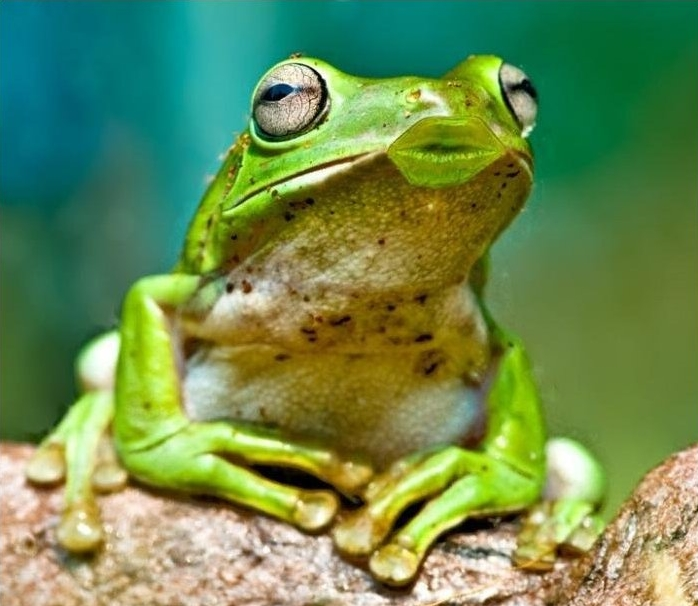
\includegraphics[width=0.6\linewidth]{C:/Users/thiago/OneDrive/UNESP/Pos_graduacao/Eco/2015/Estatistica_2015/Aulas/Aula_3_EDA_Graph/figs/sapo.jpg}
\end{figure}

\end{frame}
%===============================================================================%


%===============================================================================%
\begin{frame}{Análise Exploratória de Dados (AED)}
\setbeamercovered{transparent}  
  
\begin{itemize}

\item  É essencial ficar ``íntimo'' dos dados antes de qualquer análise \pause
\item	Você já possui um modelo conceitual (\textbf{Ou deveria\ldots}) \pause
\item	Será que seus dados se conformam a esse modelo? \pause
\item Será que seus dados foram coletados corretamente? \pause
\item Será que seus dados foram \emph{registrados} corretamente? \pause
\item Será \ldots? 
\end{itemize}


\end{frame} 
%===============================================================================%

%===============================================================================%
\begin{frame}[fragile]{Análise Exploratória de Dados (AED)}

\begin{knitrout}\tiny
\definecolor{shadecolor}{rgb}{0.969, 0.969, 0.969}\color{fgcolor}\begin{kframe}
\begin{alltt}
\hlkwd{summary}\hlstd{(m1)}
\end{alltt}
\begin{verbatim}
## 
## Call:
## lm(formula = y ~ x)
## 
## Residuals:
##     Min      1Q  Median      3Q     Max 
## -6.2944 -2.2683 -0.1736  1.8512  7.1844 
## 
## Coefficients:
##             Estimate Std. Error t value Pr(>|t|)    
## (Intercept) -0.04236    0.79101  -0.054    0.958    
## x            1.07306    0.03693  29.054   <2e-16 ***
## ---
## Signif. codes:  0 '***' 0.001 '**' 0.01 '*' 0.05 '.' 0.1 ' ' 1
## 
## Residual standard error: 2.918 on 38 degrees of freedom
## Multiple R-squared:  0.9569,	Adjusted R-squared:  0.9558 
## F-statistic: 844.2 on 1 and 38 DF,  p-value: < 2.2e-16
\end{verbatim}
\end{kframe}
\end{knitrout}


\end{frame} 
%===============================================================================%
% 
%===============================================================================%
\begin{frame}{Análise Exploratória de Dados (AED)}

\begin{knitrout}\scriptsize
\definecolor{shadecolor}{rgb}{0.969, 0.969, 0.969}\color{fgcolor}\begin{kframe}
\begin{alltt}
\hlstd{x} \hlkwb{<-} \hlkwd{c}\hlstd{(}\hlkwd{rnorm}\hlstd{(}\hlnum{20}\hlstd{,}\hlnum{5}\hlstd{,}\hlnum{1}\hlstd{),}\hlkwd{rnorm}\hlstd{(}\hlnum{20}\hlstd{,}\hlnum{30}\hlstd{,}\hlnum{1}\hlstd{))}

\hlstd{y} \hlkwb{<-} \hlstd{x} \hlopt{+} \hlkwd{rnorm}\hlstd{(}\hlnum{40}\hlstd{,}\hlnum{0}\hlstd{,}\hlnum{3}\hlstd{)}
\end{alltt}
\end{kframe}
\end{knitrout}

\centering
\begin{knitrout}
\definecolor{shadecolor}{rgb}{0.969, 0.969, 0.969}\color{fgcolor}
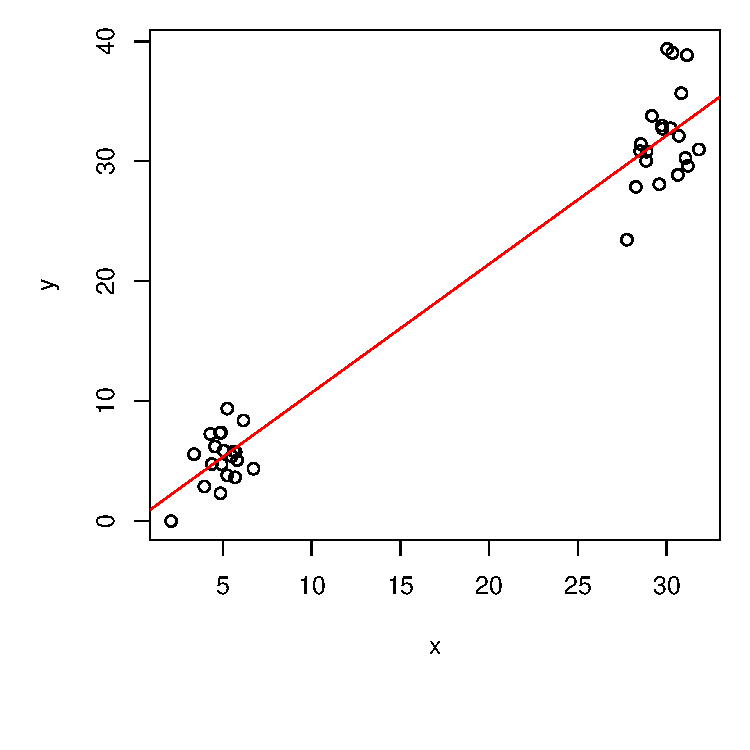
\includegraphics[width=0.6\linewidth]{figure/bolasplot-1} 

\end{knitrout}



\end{frame} 
%===============================================================================%



%===============================================================================%
\begin{frame}[fragile]{Análise Exploratória de Dados (AED)}

\begin{knitrout}\tiny
\definecolor{shadecolor}{rgb}{0.969, 0.969, 0.969}\color{fgcolor}\begin{kframe}
\begin{alltt}
\hlkwd{summary}\hlstd{(m2)}
\end{alltt}
\begin{verbatim}
## 
## Call:
## lm(formula = y2 ~ x2)
## 
## Residuals:
##     Min      1Q  Median      3Q     Max 
## -273.08 -219.65  -72.45  210.62  488.11 
## 
## Coefficients:
##             Estimate Std. Error t value Pr(>|t|)    
## (Intercept)  271.285     34.386   7.889 3.24e-10 ***
## x2             1.185      2.969   0.399    0.692    
## ---
## Signif. codes:  0 '***' 0.001 '**' 0.01 '*' 0.05 '.' 0.1 ' ' 1
## 
## Residual standard error: 243.1 on 48 degrees of freedom
## Multiple R-squared:  0.003305,	Adjusted R-squared:  -0.01746 
## F-statistic: 0.1592 on 1 and 48 DF,  p-value: 0.6917
\end{verbatim}
\end{kframe}
\end{knitrout}


\end{frame} 
%===============================================================================%

%===============================================================================%
\begin{frame}{Análise Exploratória de Dados (AED)}

\begin{knitrout}\scriptsize
\definecolor{shadecolor}{rgb}{0.969, 0.969, 0.969}\color{fgcolor}\begin{kframe}
\begin{alltt}
\hlstd{x2} \hlkwb{<-} \hlkwd{runif}\hlstd{(}\hlnum{50}\hlstd{,}\hlopt{-}\hlnum{20}\hlstd{,}\hlnum{20}\hlstd{)}

\hlstd{y2} \hlkwb{<-} \hlnum{2} \hlopt{+} \hlnum{3}\hlopt{*}\hlstd{x2} \hlopt{+} \hlstd{(}\hlnum{2}\hlopt{*}\hlstd{x2}\hlopt{^}\hlnum{2}\hlstd{)} \hlopt{+} \hlkwd{rnorm}\hlstd{(}\hlnum{50}\hlstd{,}\hlnum{0}\hlstd{,}\hlnum{3}\hlstd{)}
\end{alltt}
\end{kframe}
\end{knitrout}

\centering
\begin{knitrout}
\definecolor{shadecolor}{rgb}{0.969, 0.969, 0.969}\color{fgcolor}
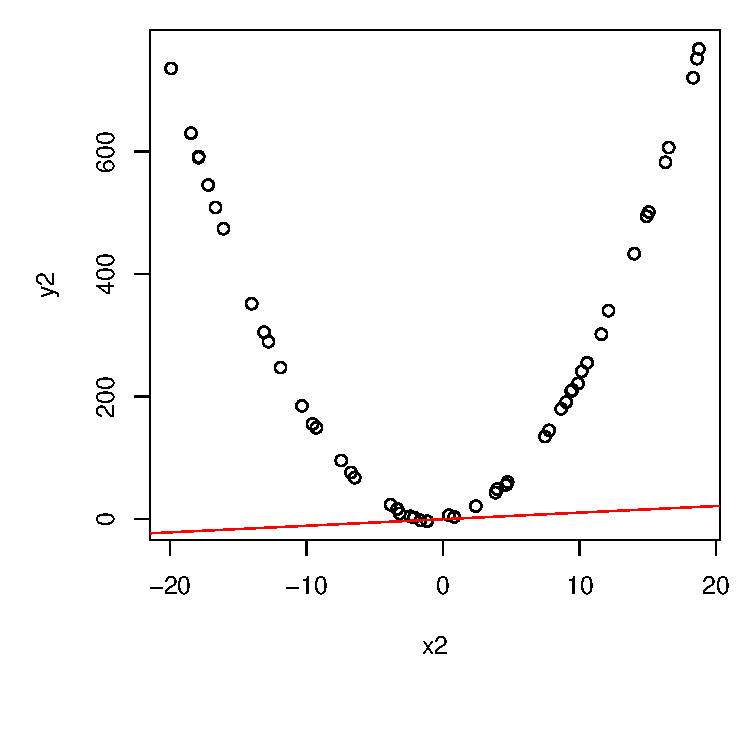
\includegraphics[width=0.6\linewidth]{figure/ushapeplot-1} 

\end{knitrout}

\end{frame} 
%===============================================================================%




%===============================================================================%
\begin{frame}[fragile]{Análise Exploratória de Dados (AED)}

\textbf{"O Quarteto de Anscombe"}

\scriptsize{Anscombe, F.J., 1973. Graphs in Statistical Analysis. The American Statistician 27, 17–21.}

\begin{columns}[c]

\column{0.5\linewidth}

\begin{knitrout}\tiny
\definecolor{shadecolor}{rgb}{0.969, 0.969, 0.969}\color{fgcolor}\begin{kframe}
\begin{alltt}
\hlstd{m1} \hlkwb{<-} \hlkwd{lm}\hlstd{(y1} \hlopt{~} \hlstd{x1,} \hlkwc{data} \hlstd{= ans)}

\hlstd{m1}\hlopt{$}\hlstd{coefficients}
\end{alltt}
\begin{verbatim}
## (Intercept)          x1 
##   3.0000909   0.5000909
\end{verbatim}
\begin{alltt}
\hlstd{m2} \hlkwb{<-} \hlkwd{lm}\hlstd{(y2} \hlopt{~} \hlstd{x2,} \hlkwc{data} \hlstd{= ans)}

\hlstd{m2}\hlopt{$}\hlstd{coefficients}
\end{alltt}
\begin{verbatim}
## (Intercept)          x2 
##    3.000909    0.500000
\end{verbatim}
\end{kframe}
\end{knitrout}

\column{0.5\linewidth}

\begin{knitrout}\tiny
\definecolor{shadecolor}{rgb}{0.969, 0.969, 0.969}\color{fgcolor}\begin{kframe}
\begin{alltt}
\hlstd{m3} \hlkwb{<-} \hlkwd{lm}\hlstd{(y3} \hlopt{~} \hlstd{x3,} \hlkwc{data} \hlstd{= ans)}

\hlstd{m3}\hlopt{$}\hlstd{coefficients}
\end{alltt}
\begin{verbatim}
## (Intercept)          x3 
##   3.0024545   0.4997273
\end{verbatim}
\begin{alltt}
\hlstd{m4} \hlkwb{<-} \hlkwd{lm}\hlstd{(y4} \hlopt{~} \hlstd{x4,} \hlkwc{data} \hlstd{= ans)}

\hlstd{m4}\hlopt{$}\hlstd{coefficients}
\end{alltt}
\begin{verbatim}
## (Intercept)          x4 
##   3.0017273   0.4999091
\end{verbatim}
\end{kframe}
\end{knitrout}

\end{columns}

\end{frame} 
%===============================================================================%


%===============================================================================%
\begin{frame}[fragile]{O Quarteto de Anscombe}

\begin{columns}[c]

\column{0.5\linewidth}

\begin{knitrout}
\definecolor{shadecolor}{rgb}{0.969, 0.969, 0.969}\color{fgcolor}
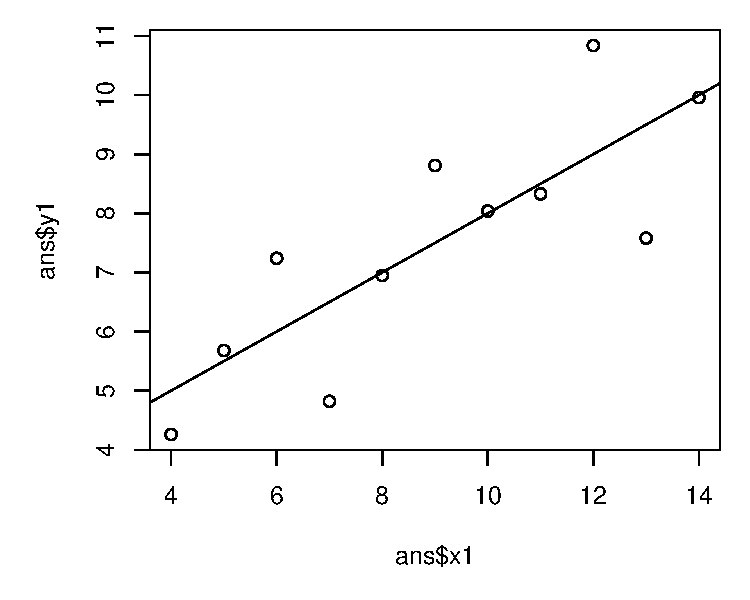
\includegraphics[width=0.9\linewidth]{figure/ans12-1} 

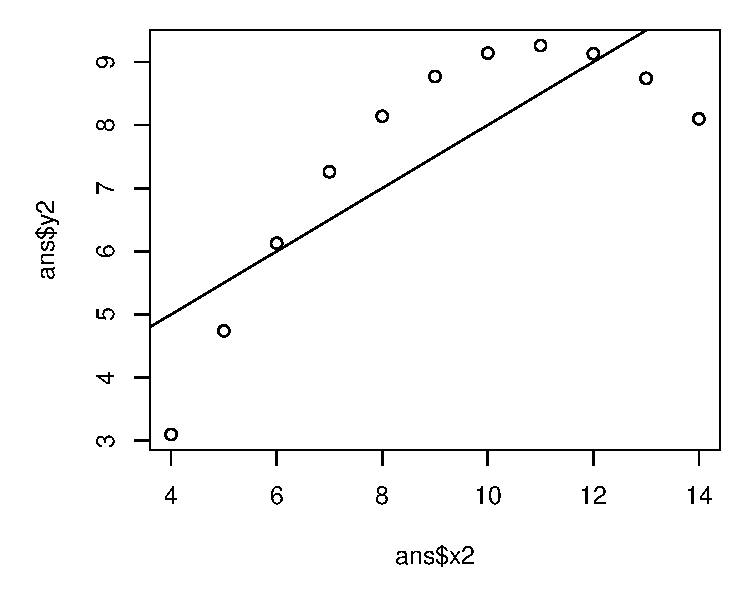
\includegraphics[width=0.9\linewidth]{figure/ans12-2} 

\end{knitrout}

\column{0.5\linewidth}

\begin{knitrout}
\definecolor{shadecolor}{rgb}{0.969, 0.969, 0.969}\color{fgcolor}
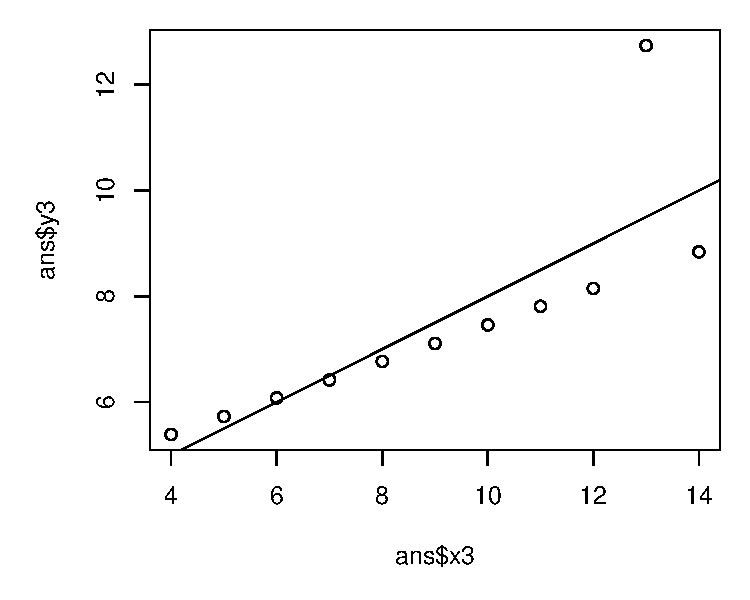
\includegraphics[width=0.9\linewidth]{figure/an34-1} 

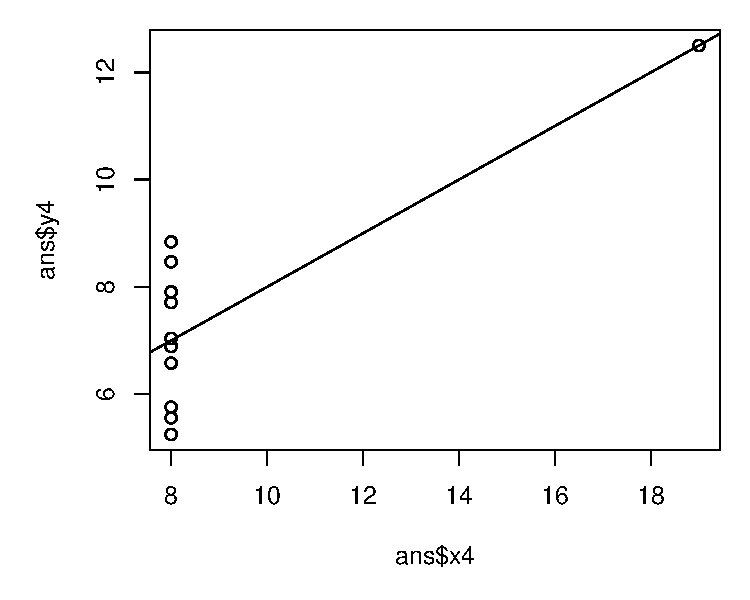
\includegraphics[width=0.9\linewidth]{figure/an34-2} 

\end{knitrout}

\end{columns}

\end{frame} 
%===============================================================================%


%===============================================================================%
\begin{frame}{Análise Exploratória de Dados (AED)}
%\setbeamercovered{transparent}  
\linespread{1.5} 
 
 A Análise Exploratória é normalmente composta por:
 
\begin{itemize}

\item \textbf{Estatísticas Descritivas}
\item	\textbf{Análise Gráfica}
\item  Aderência à distribuição
\item Análise de Relações

\end{itemize}


\end{frame} 
%===============================================================================%

\section{Codificação e organização de dados}
% 
% %=============================================================================%
% \begin{frame}{Codificação de Variáveis}{Teoria da mensuração}
% 
% \begin{tikzpicture}[grow=right]
%   \tikzset{level distance=80pt,sibling distance=5pt}
%   \tikzset{execute at begin node=\strut}
%   \tikzset{every tree node/.style={anchor=base west}}
%   \only<1>{\Tree [.Variáveis Qualitativas(Categóricas) Quantitativas ]}
%   \only<2>{\Tree [.Variáveis [.Qualitativas Nominais Ordinais ] Quantitativas ]}
%   \only<3>{\Tree [.Variáveis [.Qualitativas [.Nominais (Binárias) ] Ordinais ] Quantitativas ]}
%   \only<4>{\Tree [.Variáveis [.Qualitativas Binárias Nominais Ordinais ] Quantitativas ] [.Quantitativas Intervalo Razão ]]}
%   \only<5>{\Tree [.Variáveis [.Qualitativas Binárias Nominais Ordinais ] [.Quantitativas \alert{Discretas} \alert{Contínuas} ]]}
% \end{tikzpicture}
% 
% \end{frame}
% % %===============================================================================%
% 
% 
% 
% %===============================================================================%
% \begin{frame}{Codificação de Variáveis}{Exemplos}
% %\setbeamercovered{transparent}  
% \linespread{1.5} 
%  
% \begin{itemize}
% 
% \item \textbf{Binária:} Sim/Não, Masculino/Feminino
% \item \textbf{Nominal:} Esquerda/Direita/Centro, Floresta/Água/Solo
% \item	\textbf{Ordinal:} Ruim/Médio/Bom, Baixo/Médio/Alto
% \item \textbf{Intervalo:} Temperatura ($^{\circ}\mathrm{C}$) (intervalos iguais, sem zero absoluto, razões não fazem sentido) 
% \item \textbf{Razão(\emph{Ratio}):} temperatura (K), altura (m), peso (g) (intervalos iguais, zero abosoluto, razões fazem sentido)
% 
% \end{itemize}
% 
% 
% \end{frame} 
% %===============================================================================%

%===============================================================================%
\begin{frame}[fragile]{Organizando tabelas de dados}

\begin{Small}
\begin{itemize}
  \item Na maioria das vezes, recebemos ou tabulamos nossos dados no formato \emph{wide} (largo)
  \item Mas a maioria dos pacotes de análise requer tabelas no formato \emph{long} (longo) 
  \item Exemplo: um estudo de lagos em ambientes litorâneos, interiores e montanhosos
\end{itemize}




\begin{tiny}
% latex table generated in R 3.1.3 by xtable 1.7-4 package
% Fri Aug 28 15:57:28 2015
\begin{table}[ht]
\centering
\begin{tabular}{rlrrrr}
  \hline
 & Lago & Tinv & Tver & Phinv & Phver \\ 
  \hline
1 & L1 & 20.32 & 28.35 & 6.50 & 7.07 \\ 
  2 & L2 & 19.63 & 27.33 & 6.82 & 7.26 \\ 
  3 & L3 & 20.99 & 26.05 & 7.11 & 7.08 \\ 
  4 & L4 & 20.31 & 26.13 & 8.00 & 5.28 \\ 
  5 & L5 & 20.13 & 26.54 & 6.56 & 6.58 \\ 
  6 & L6 & 19.93 & 26.53 & 7.46 & 8.05 \\ 
  7 & L7 & 20.95 & 24.63 & 7.25 & 7.15 \\ 
  8 & L8 & 21.13 & 27.25 & 7.06 & 6.77 \\ 
  9 & L9 & 19.70 & 26.82 & 6.70 & 6.59 \\ 
  10 & L10 & 20.04 & 27.90 & 5.92 & 6.91 \\ 
   \hline
\end{tabular}
\caption{Lagos litorâneos} 
\end{table}

\end{tiny}

% \begin{itemize} \pause
%   \item{\textbf{Quantas variáveis existem nessa tabela?}}
% \end{item}

\end{Small}
\end{frame}
%===============================================================================%

%===============================================================================%
\begin{frame}[fragile]



\begin{tiny}
% latex table generated in R 3.1.3 by xtable 1.7-4 package
% Fri Aug 28 15:57:28 2015
\begin{table}[ht]
\centering
\begin{tabular}{rlrrrr}
  \hline
 & Lago & Tinv & Tver & Phinv & Phver \\ 
  \hline
1 & L11 & 14.99 & 23.41 & 6.37 & 6.60 \\ 
  2 & L12 & 14.35 & 22.82 & 5.50 & 7.40 \\ 
  3 & L13 & 14.22 & 23.39 & 6.39 & 7.71 \\ 
  4 & L14 & 15.44 & 22.59 & 6.74 & 6.81 \\ 
  5 & L15 & 14.23 & 23.70 & 6.63 & 7.45 \\ 
  6 & L16 & 14.83 & 22.29 & 6.11 & 6.77 \\ 
  7 & L17 & 15.93 & 23.06 & 8.07 & 7.28 \\ 
  8 & L18 & 14.17 & 22.11 & 7.03 & 6.65 \\ 
  9 & L19 & 14.78 & 23.94 & 6.55 & 7.15 \\ 
  10 & L20 & 14.73 & 23.68 & 6.93 & 5.93 \\ 
   \hline
\end{tabular}
\caption{Lagos interiores} 
\end{table}

\end{tiny}

\end{frame}
%===============================================================================%


%===============================================================================%
\begin{frame}[fragile]



\begin{tiny}
% latex table generated in R 3.1.3 by xtable 1.7-4 package
% Fri Aug 28 15:57:28 2015
\begin{table}[ht]
\centering
\begin{tabular}{rlrrrr}
  \hline
 & Lago & Tinv & Tver & Phinv & Phver \\ 
  \hline
1 & L21 & 9.83 & 22.70 & 6.78 & 7.40 \\ 
  2 & L22 & 10.13 & 22.95 & 7.19 & 6.76 \\ 
  3 & L23 & 10.65 & 22.89 & 6.93 & 6.27 \\ 
  4 & L24 & 8.99 & 22.56 & 7.10 & 6.55 \\ 
  5 & L25 & 9.81 & 21.31 & 6.56 & 7.26 \\ 
  6 & L26 & 8.86 & 22.76 & 6.69 & 7.26 \\ 
  7 & L27 & 9.84 & 22.08 & 6.69 & 7.07 \\ 
  8 & L28 & 9.16 & 23.34 & 7.38 & 7.71 \\ 
  9 & L29 & 10.90 & 20.33 & 7.98 & 7.15 \\ 
  10 & L30 & 10.43 & 21.62 & 7.30 & 6.75 \\ 
   \hline
\end{tabular}
\caption{Lagos de montanha} 
\end{table}

\end{tiny}
\end{frame}
%===============================================================================%

%===============================================================================%
\begin{frame}
\centering
\textbf{Quantas variáveis possui esse estudo?}
\end{frame}
%===============================================================================%

%===============================================================================%
\begin{frame}{Quantas variáveis?}

\begin{itemize}
  \item Lago (L1, L2,\ldots - poderia ser analisada se tomássemos várias observações por lago) \pause
  \item Região (Litoral, Interior, Montanha) \pause
  \item Estação (Inverno, Verão) \pause
  \item Temperatura \pause
  \item pH
\end{itemize}

\end{frame}
%===============================================================================%


%===============================================================================%
\begin{frame}[fragile]

\begin{itemize}
  \item No formato longo, cada coluna descreve uma variável, e cada linha representa uma observação:
\end{itemize} \pause

\begin{knitrout}\tiny
\definecolor{shadecolor}{rgb}{0.969, 0.969, 0.969}\color{fgcolor}\begin{kframe}
\begin{alltt}
\hlstd{lago.long} \hlkwb{<-} \hlkwd{read.csv}\hlstd{(}\hlstr{'lakedata_long.csv'}\hlstd{)}
\end{alltt}
\end{kframe}
\end{knitrout}

\begin{tiny}
\begin{table}[ht]
\centering
\begin{tabular}{rlllrr}
  \hline
 & Lago & Regiao & Estacao & Temp & pH \\ 
  \hline
1 & L1 & Litoral & Inverno & 20.32 & 6.50 \\ 
  2 & L2 & Litoral & Inverno & 19.63 & 6.82 \\ 
  3 & L3 & Litoral & Inverno & 20.99 & 7.11 \\ 
  4 & L4 & Litoral & Inverno & 20.31 & 8.00 \\ 
  5 & L5 & Litoral & Inverno & 20.13 & 6.56 \\ 
  6 & L6 & Litoral & Inverno & 19.93 & 7.46 \\ 
  7 & L7 & Litoral & Inverno & 20.95 & 7.25 \\ 
  8 & L8 & Litoral & Inverno & 21.13 & 7.06 \\ 
  9 & L9 & Litoral & Inverno & 19.70 & 6.70 \\ 
  10 & L10 & Litoral & Inverno & 20.04 & 5.92 \\ 
  11 & L11 & Interior & Inverno & 14.99 & 6.37 \\ 
  12 & L12 & Interior & Inverno & 14.35 & 5.50 \\ 
   \ldots & \ldots & \ldots & \ldots & \ldots & \ldots \\
   54 & L24 & Montanha & Verao & 22.56 & 6.55 \\ 
  55 & L25 & Montanha & Verao & 21.31 & 7.26 \\ 
  56 & L26 & Montanha & Verao & 22.76 & 7.26 \\ 
  57 & L27 & Montanha & Verao & 22.08 & 7.07 \\ 
  58 & L28 & Montanha & Verao & 23.34 & 7.71 \\ 
  59 & L29 & Montanha & Verao & 20.33 & 7.15 \\ 
  60 & L30 & Montanha & Verao & 21.62 & 6.75 \\ 
   \hline
\end{tabular}
\end{table}
\end{tiny}

\end{frame}

%===============================================================================%


\section{Estatística Descritiva}

%===============================================================================%
\begin{frame}{Estatística Descritiva: tendência central e dispersão}
%\setbeamercovered{transparent}  
\linespread{1.5} 
 
Através da estatística descritiva, buscamos: 
 
\begin{itemize}

\item \emph{Localizar} nossos dados no espaço (numérico)
\begin{itemize}
  \item Quais os valores \emph{esperados} para estes dados?
\end{itemize}
\vfill
\item  Quantificar a \emph{dispersão} destes dados em torno desta localidade
\begin{itemize}
  \item Qual a \emph{variância} dos meus dados?
\end{itemize}
\end{itemize}

\end{frame} 
%===============================================================================%


%===============================================================================%
\begin{frame}{Estatística Descritiva: tendência central e dispersão}
%\setbeamercovered{transparent}  
\linespread{1.5} 
 
\textbf{Tendência central para dados contínuos?}

\begin{columns}[c]

\column{0.6\linewidth}

\begin{itemize}
  \only<2>{\item Média}
%   \only<3-4>{\item \textcolor{gray}{Média aritmética}}
%   \only<3>{\item Média geométrica}
%   \only<4-4>{\item \textcolor{gray}{Média geométrica}}
%   \only<4-4>{\item Média harmônica}
\end{itemize}

\column{0.4\linewidth}

\only<2>{
\begin{equation*}
  \bar X_{(arit)} = \frac{1}{n} \sum_{i=1}^{n} x_i
\end{equation*}
}

% \only<3>{
% \begin{equation*}
%   \bar X_{(geom)} = \left(\prod_{i=1}^{n}{x_i}\right)^\frac{1}{n} 
% \end{equation*}
% }
% 
% \only<3>{
% \begin{equation*}
%   \bar X_{(geom)} = \exp\left({\alert{\frac{1}{n}\sum_{i=1}^{n}} \log{x_i}}\right)
% \end{equation*}
% }
% 
% 
% \only<4>{
% \begin{equation*}
%   \bar X = \left(\alert{\frac{1}{n}\sum_{i=1}^{n}}\frac{1}{x_i}\right)^{-1}
% \end{equation*}
% }

\end{columns}

\end{frame} 
%===============================================================================%

% %===============================================================================%
% \begin{frame}{Tendência Central: Exemplos}
% 
% \begin{block}{Média Aritmética: para variáveis que se somam (efeitos aditivos)}
%   Se eu tenho três pacotes, de 1kg, 6kg, e 3kg, quanto carrego de peso em média?
%   
%   \vspace{10 mm}
%   
%   $\frac{1 + 6 + 3}{3} = mean(c(1,6,3))$
%   
%   \vspace{10 mm}
%   
%   Ou seja, seria o mesmo que carregar 3 pacotes de mean(c(1,6,3))kg \txtbf{somados}
% \end{block}
% 
% \end{frame}
% %===============================================================================%
% 
% 
% %===============================================================================%
% \begin{frame}{Tendência Central: Exemplos}
% 
% \begin{small}
% \begin{block}{Média Geométrica: para variáveis que se multiplicam (efeitos cumulativos)}
%   Se sua bolsa de mestrado recebe um aumento de 1\% no primeiro ano, 6\% no segundo ano, e 3\% no terceiro ano, qual é o aumento médio nos 3 anos?
%    
%  \vspace{3 mm}
%    
% Bolsa final: R\$ $1500 * 1.01 * 1.06 * 1.03 =$ R\$ round(1500 * 1.01*1.06*1.03,0)
% 
%  \vspace{3 mm}
%    
%    $(1.01 * 1.06 * 1.03)^\frac{1}{3} = 1.01*1.06*1.03^\frac{1}{3} = (prod(c(1.01,1.06,1.03)))^(1/3)$
%  
%  \vspace{3 mm}
%  
%     Ou seja, o aumento percentual médio foi de -((1-(prod(c(1.01,1.06,1.03))^(1/3)))*100) \%
%   
%   \vspace{5 mm}
%   
% Redimento: $1500 * 1.0331 * 1.0331 * 1.0331= round(1500 * 1.0331*1.0331*1.0331,0)$\pause
% 
% Aritmética: \alert{$1500 * 1.0333 * 1.0333 * 1.0333 = round(1500 * 1.0333*1.0333*1.0333,0)$}
% \end{block}
% \end{small}
% 
% \end{frame}
% %===============================================================================%
% 
% 
% %===============================================================================%
% \begin{frame}{Tendência Central: Exemplos}
% 
% \begin{small}
% \begin{block}{Média Harmônica: para proporções (recíprocos)}
%  Você viaja de carro por 300km, a 20km/h nos primeiros 100km, a 40km/h nos próximos 100km, e finalmente a 80km/h nos 100km finais. Que velocidade você deveria manter constante para percorrer os mesmos 300km, no mesmo tempo?
%    
%  \vspace{3 mm}
%  
%   Parte 1: 100/20 = 5h; Parte 2: 100/40 = 2.5h; 100/80 = 1.25h; Tempo total =8.75h
%  
%   \vspace{3 mm}
%    
%    $\leff(\left(\frac{1}{3} \times \left(\frac{1}{20} + \frac{1}{40} + \frac{1}{80}\right)\right)^{-1} = (mean(c(1/20,1/40,1/80)))^-1$
%  
%  \vspace{3 mm}
%  
%     Ou seja, uma velocidade média de (mean(1/c(20,40,80)))^-1 km/h
%   
%   \vspace{3 mm}
%   
% Distancia: (mean(1/c(20,40,80)))^-1 * 8.75 = ((mean(1/c(20,40,80)))^-1)*8.75\pause
% 
% Aritmética: \alert{mean(c(20,40,80)) * 8.75  = mean(c(20,40,80))*8.75}
% \end{block}
% 
% \end{small}
% \end{frame}
% %===============================================================================%


%===============================================================================%
\begin{frame}{Estatística Descritiva: tendência central e dispersão}
 
\textbf{Dispersão para dados contínuos?}

\begin{columns}[T]

\column{0.6\linewidth}

\begin{itemize}
  \only<2>{\item Variância e Desvio Padrão}
  \only<3-4>{\item \textcolor{gray}{Variância e Desvio Padrão}}
  \only<3>{\item Amplitude}
  \only<4-4>{\item \textcolor{gray}{Amplitude}}
  \only<4-4>{\item Coeficiente de Variação}
\end{itemize}

\column{0.4\linewidth}

\only<2>{
\begin{equation*}
 s^2 = \frac{1}{n-1} \sum_{i=1}^{n} (x_i - \bar x)^2
\end{equation*}
}

\only<2>{
\begin{equation*}
 s = \sqrt{s^2}
\end{equation*}
}

\only<3>{
\begin{equation*}
  A = max(x) - min(x)
\end{equation*}
}

\only<4>{
\begin{equation*}
  CV = \frac{s}{\bar x} * 100 (\%)
\end{equation*}
}

\end{columns}

\end{frame} 
%===============================================================================%


%===============================================================================%
\begin{frame}[fragile]%{Tendência Central: Distribuição Normal}

\begin{columns}[c]

\column{0.49\linewidth}

\begin{knitrout}\tiny
\definecolor{shadecolor}{rgb}{0.969, 0.969, 0.969}\color{fgcolor}\begin{kframe}
\begin{alltt}
\hlkwd{set.seed}\hlstd{(}\hlnum{1979}\hlstd{)}
\hlstd{x} \hlkwb{<-} \hlkwd{rnorm}\hlstd{(}\hlnum{500}\hlstd{,}\hlnum{50}\hlstd{,}\hlnum{10}\hlstd{)}
\hlstd{cv} \hlkwb{<-} \hlkwa{function}\hlstd{(}\hlkwc{x}\hlstd{)} \hlkwd{sd}\hlstd{(x)}\hlopt{/}\hlkwd{mean}\hlstd{(x)} \hlopt{*} \hlnum{100}
\hlkwd{mean}\hlstd{(x)}
\end{alltt}
\begin{verbatim}
## [1] 50.36405
\end{verbatim}
\begin{alltt}
\hlkwd{sd}\hlstd{(x)}
\end{alltt}
\begin{verbatim}
## [1] 9.877513
\end{verbatim}
\begin{alltt}
\hlkwd{cv}\hlstd{(x)}
\end{alltt}
\begin{verbatim}
## [1] 19.61223
\end{verbatim}
\begin{alltt}
\hlkwd{hist}\hlstd{(x,}\hlkwc{breaks}\hlstd{=}\hlnum{40}\hlstd{,}\hlkwc{prob}\hlstd{=T,}\hlkwc{xlim}\hlstd{=}\hlkwd{c}\hlstd{(}\hlnum{0}\hlstd{,}\hlnum{100}\hlstd{),}\hlkwc{col}\hlstd{=}\hlstr{'gray70'}\hlstd{)}
\hlkwd{curve}\hlstd{(}\hlkwd{dnorm}\hlstd{(x,}\hlkwc{mean}\hlstd{=}\hlnum{50}\hlstd{,} \hlkwc{sd}\hlstd{=}\hlnum{10}\hlstd{),} \hlkwc{add}\hlstd{=T)}
\hlkwd{abline}\hlstd{(}\hlkwc{v}\hlstd{=}\hlkwd{mean}\hlstd{(x),}\hlkwc{col}\hlstd{=}\hlstr{'red'}\hlstd{)}
\hlkwd{abline}\hlstd{(}\hlkwc{v}\hlstd{=}\hlkwd{c}\hlstd{(}\hlkwd{mean}\hlstd{(x)}\hlopt{+}\hlkwd{sd}\hlstd{(x),}\hlkwd{mean}\hlstd{(x)}\hlopt{-}\hlkwd{sd}\hlstd{(x)),}\hlkwc{col}\hlstd{=}\hlstr{'blue'}\hlstd{)}
\hlkwd{abline}\hlstd{(}\hlkwc{v}\hlstd{=}\hlkwd{c}\hlstd{(}\hlkwd{mean}\hlstd{(x)}\hlopt{+}\hlnum{2}\hlopt{*}\hlkwd{sd}\hlstd{(x),}\hlkwd{mean}\hlstd{(x)}\hlopt{-}\hlnum{2}\hlopt{*}\hlkwd{sd}\hlstd{(x)),}\hlkwc{col}\hlstd{=}\hlstr{'purple'}\hlstd{)}
\end{alltt}
\end{kframe}
\end{knitrout}

\column{0.5\linewidth}
\centering
\begin{knitrout}
\definecolor{shadecolor}{rgb}{0.969, 0.969, 0.969}\color{fgcolor}
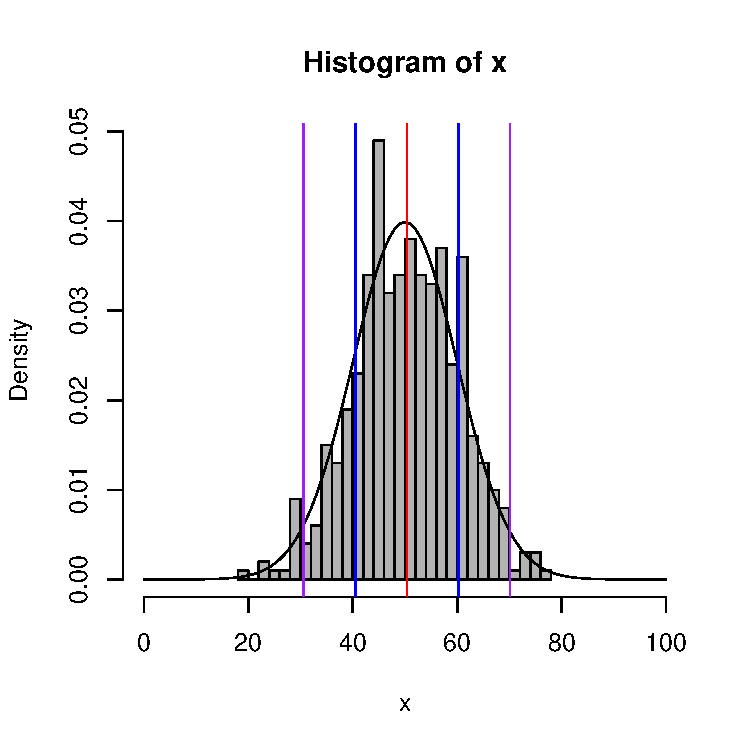
\includegraphics[width=1.1\linewidth]{figure/unnamed-chunk-4-1} 

\end{knitrout}

\end{columns}

\end{frame} 
%===============================================================================%


%===============================================================================%
\begin{frame}[fragile]%{Tendência Central: Distribuição Normal}

\begin{columns}[c]

\column{0.49\linewidth}

\begin{knitrout}\tiny
\definecolor{shadecolor}{rgb}{0.969, 0.969, 0.969}\color{fgcolor}\begin{kframe}
\begin{alltt}
\hlkwd{set.seed}\hlstd{(}\hlnum{1979}\hlstd{)}
\hlstd{x} \hlkwb{<-} \hlkwd{rnorm}\hlstd{(}\hlnum{500}\hlstd{,}\hlnum{50}\hlstd{,}\hlnum{20}\hlstd{)}
\hlstd{cv} \hlkwb{<-} \hlkwa{function}\hlstd{(}\hlkwc{x}\hlstd{)} \hlkwd{sd}\hlstd{(x)}\hlopt{/}\hlkwd{mean}\hlstd{(x)} \hlopt{*} \hlnum{100}
\hlkwd{mean}\hlstd{(x)}
\end{alltt}
\begin{verbatim}
## [1] 50.7281
\end{verbatim}
\begin{alltt}
\hlkwd{sd}\hlstd{(x)}
\end{alltt}
\begin{verbatim}
## [1] 19.75503
\end{verbatim}
\begin{alltt}
\hlkwd{cv}\hlstd{(x)}
\end{alltt}
\begin{verbatim}
## [1] 38.94297
\end{verbatim}
\begin{alltt}
\hlcom{## hist(x,breaks=40,prob=T,xlim=c(0,100),col='gray70')}
\hlcom{## curve(dnorm(x,mean=50, sd=20), add=T)}
\hlcom{## abline(v=mean(x),col='red')}
\hlcom{## abline(v=c(mean(x)+sd(x),mean(x)-sd(x)),col='blue')}
\hlcom{## abline(v=c(mean(x)+2*sd(x),mean(x)-2*sd(x)),col='purple')}
\end{alltt}
\end{kframe}
\end{knitrout}

\column{0.5\linewidth}
\centering
\begin{knitrout}
\definecolor{shadecolor}{rgb}{0.969, 0.969, 0.969}\color{fgcolor}
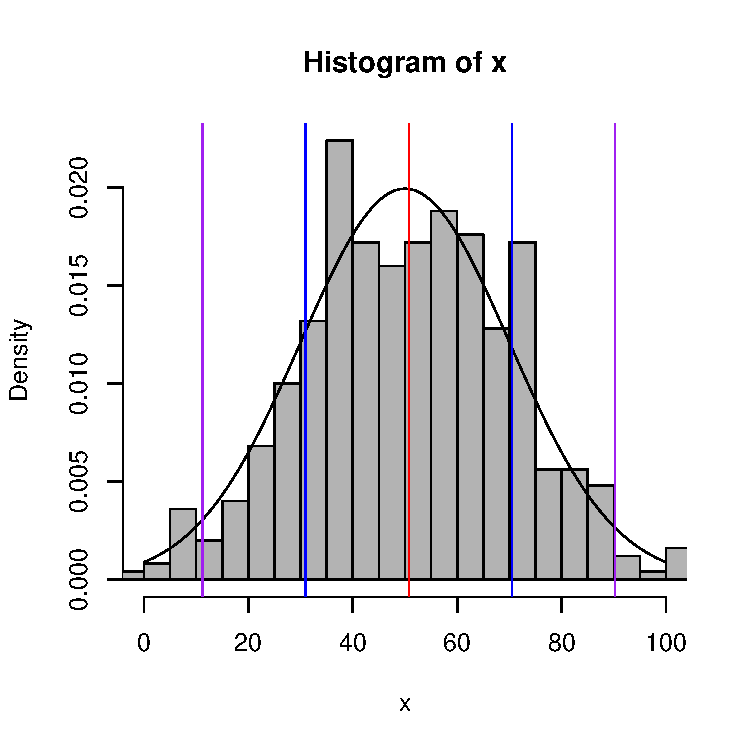
\includegraphics[width=1.1\linewidth]{figure/unnamed-chunk-6-1} 

\end{knitrout}

\end{columns}

\end{frame} 
%===============================================================================%


%===============================================================================%
\begin{frame}{Estatística Descritiva: desvio padrão}

\begin{columns}[c]

\column{0.49\linewidth}

A regra do $68$-$95$-$99.7$

Para uma distribuição normal

\begin{itemize}

  \item $1 \times s \approx 68$ \% dos dados
  \item $2 \times s \approx 95$ \% dos dados
  \item $3 \times s \approx 99.7$ \% dos dados

\end{itemize}
\column{0.5\linewidth}
\centering
\begin{knitrout}
\definecolor{shadecolor}{rgb}{0.969, 0.969, 0.969}\color{fgcolor}
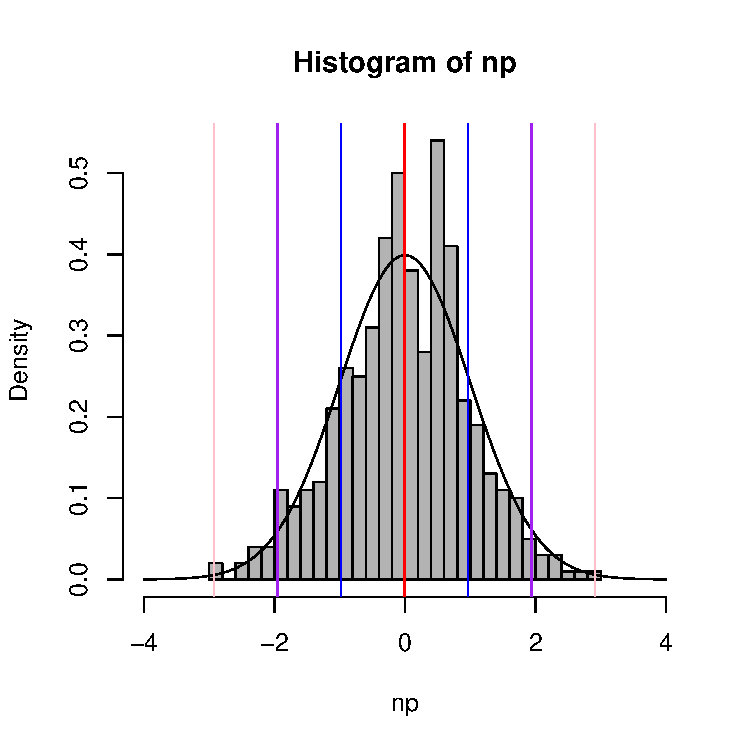
\includegraphics[width=1.1\linewidth]{figure/unnamed-chunk-7-1} 

\end{knitrout}

\end{columns}


\end{frame} 
%===============================================================================%



%===============================================================================%
\begin{frame}{Estatística Descritiva: tendência central e dispersão}
\setbeamercovered{transparent}  

\textbf{Percentis (\emph{Percentiles}): medidas robustas de tendência central e dispersão}

$k$-ésimo percentil = $k$\% de $n$ está abaixo desse valor, $(100-k)$\% de $n$ está acima desse valor

\pause

\begin{itemize}
  \item \textbf{Mediana}: $k= 50$\%, $100-k =50$\%
   
\end{itemize}

\end{frame} 
%===============================================================================%


%===============================================================================%
\begin{frame}{Estatística Descritiva: tendência central e dispersão}
\setbeamercovered{transparent}  

\alert{Problema:} nem sempre existe um valor que satisfaça a condição, para um dado $k$

$ x = [1, 2, 4, 33, 200]$

$k(0\%) = 1$

$k(25\%) = 2$

$k(50\%) = 4$

$k(75\%) = 33$

$k(100\%) = 200$

$k(95\%) = ?$

\end{frame} 
%===============================================================================%

%===============================================================================%
\begin{frame}{Estatística Descritiva: tendência central e dispersão}
\setbeamercovered{transparent}  

\textbf{Quantis (\emph{Quantiles}): podem ser calculados para qualquer amostra}

$Q(p) = x:P(X < x) \leq p; P(X > x) \geq (1-p)$

Se não há valores que satisfazem essa condição, o valor é interpolado proporcionalmente à distância entre os percentis dos valores $x_i$ e $x_{i+1}$ que enquadram o quantil desejado.
\pause

\begin{itemize}
  \item \textbf{Mediana}: $Q(0.5)$
  \item \textbf{Quartil Superior}: $Q(0.75)$
  \item \textbf{Quartil Inferior}: $Q(0.25)$
   
\end{itemize}

\end{frame} 
%===============================================================================%


%===============================================================================%
\begin{frame}[fragile]%{Tendência Central: Distribuição Normal}

\begin{columns}[c]

\column{0.49\linewidth}

\begin{knitrout}\tiny
\definecolor{shadecolor}{rgb}{0.969, 0.969, 0.969}\color{fgcolor}\begin{kframe}
\begin{alltt}
\hlkwd{set.seed}\hlstd{(}\hlnum{1979}\hlstd{)}
\hlstd{x} \hlkwb{<-} \hlkwd{rnorm}\hlstd{(}\hlnum{500}\hlstd{,}\hlnum{50}\hlstd{,}\hlnum{20}\hlstd{)}

\hlkwd{median}\hlstd{(x)}
\end{alltt}
\begin{verbatim}
## [1] 51.39951
\end{verbatim}
\begin{alltt}
\hlkwd{quantile}\hlstd{(x,}\hlkwc{prob}\hlstd{=}\hlnum{0.5}\hlstd{)}
\end{alltt}
\begin{verbatim}
##      50% 
## 51.39951
\end{verbatim}
\begin{alltt}
\hlkwd{quantile}\hlstd{(x,}\hlkwc{prob}\hlstd{=}\hlkwd{c}\hlstd{(}\hlnum{0.25}\hlstd{,}\hlnum{0.75}\hlstd{))}
\end{alltt}
\begin{verbatim}
##      25%      75% 
## 37.76660 64.73483
\end{verbatim}
\begin{alltt}
\hlkwd{hist}\hlstd{(x,}\hlkwc{breaks}\hlstd{=}\hlnum{40}\hlstd{,}\hlkwc{prob}\hlstd{=T,}\hlkwc{xlim}\hlstd{=}\hlkwd{c}\hlstd{(}\hlnum{0}\hlstd{,}\hlnum{100}\hlstd{),}\hlkwc{col}\hlstd{=}\hlstr{'gray70'}\hlstd{)}
\hlkwd{curve}\hlstd{(}\hlkwd{dnorm}\hlstd{(x,}\hlkwc{mean}\hlstd{=}\hlnum{50}\hlstd{,} \hlkwc{sd}\hlstd{=}\hlnum{20}\hlstd{),} \hlkwc{add}\hlstd{=T)}
\hlkwd{abline}\hlstd{(}\hlkwc{v}\hlstd{=}\hlkwd{median}\hlstd{(x),}\hlkwc{col}\hlstd{=}\hlstr{'red'}\hlstd{,}\hlkwc{lwd}\hlstd{=}\hlnum{2}\hlstd{,}\hlkwc{lty}\hlstd{=}\hlnum{2}\hlstd{)}
\hlkwd{abline}\hlstd{(}\hlkwc{v}\hlstd{=}\hlkwd{quantile}\hlstd{(x,}\hlkwc{prob}\hlstd{=}\hlkwd{c}\hlstd{(}\hlnum{0.25}\hlstd{,}\hlnum{0.75}\hlstd{)),}\hlcom{#}
       \hlkwc{col}\hlstd{=}\hlstr{'blue'}\hlstd{,}\hlkwc{lwd}\hlstd{=}\hlnum{2}\hlstd{,}\hlkwc{lty}\hlstd{=}\hlnum{2}\hlstd{)}
\end{alltt}
\end{kframe}
\end{knitrout}

\column{0.5\linewidth}
\centering
\begin{knitrout}
\definecolor{shadecolor}{rgb}{0.969, 0.969, 0.969}\color{fgcolor}
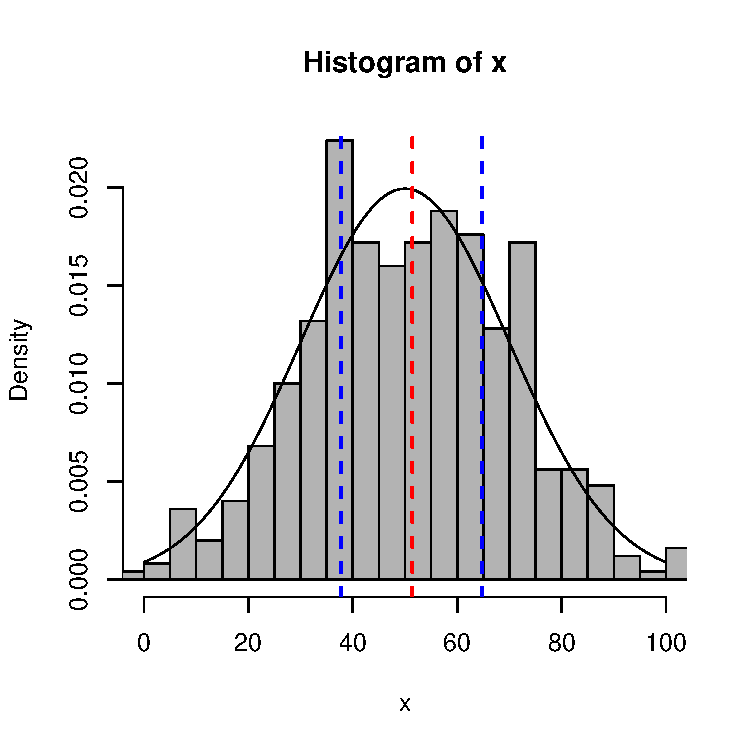
\includegraphics[width=1.1\linewidth]{figure/unnamed-chunk-9-1} 

\end{knitrout}

\end{columns}

\end{frame} 
%===============================================================================%



%===============================================================================%
\begin{frame}[fragile]%{Tendência Central: Distribuição Normal}

\begin{columns}[c]

\column{0.49\linewidth}

\begin{knitrout}\tiny
\definecolor{shadecolor}{rgb}{0.969, 0.969, 0.969}\color{fgcolor}\begin{kframe}
\begin{alltt}
\hlkwd{set.seed}\hlstd{(}\hlnum{1979}\hlstd{)}
\hlstd{x} \hlkwb{<-} \hlkwd{rnorm}\hlstd{(}\hlnum{500}\hlstd{,}\hlnum{50}\hlstd{,}\hlnum{20}\hlstd{)}

\hlkwd{hist}\hlstd{(x,}\hlkwc{breaks}\hlstd{=}\hlnum{40}\hlstd{,}\hlkwc{prob}\hlstd{=T,}\hlkwc{xlim}\hlstd{=}\hlkwd{c}\hlstd{(}\hlnum{0}\hlstd{,}\hlnum{100}\hlstd{),}\hlkwc{col}\hlstd{=}\hlstr{'gray70'}\hlstd{)}
\hlkwd{curve}\hlstd{(}\hlkwd{dnorm}\hlstd{(x,}\hlkwc{mean}\hlstd{=}\hlnum{50}\hlstd{,} \hlkwc{sd}\hlstd{=}\hlnum{20}\hlstd{),} \hlkwc{add}\hlstd{=T)}
\hlkwd{abline}\hlstd{(}\hlkwc{v}\hlstd{=}\hlkwd{mean}\hlstd{(x),}\hlkwc{col}\hlstd{=}\hlstr{'red'}\hlstd{,}\hlkwc{lwd}\hlstd{=}\hlnum{2}\hlstd{,}\hlkwc{lty}\hlstd{=}\hlnum{1}\hlstd{)}
\hlkwd{abline}\hlstd{(}\hlkwc{v}\hlstd{=}\hlkwd{median}\hlstd{(x),}\hlkwc{col}\hlstd{=}\hlstr{'red'}\hlstd{,}\hlkwc{lwd}\hlstd{=}\hlnum{2}\hlstd{,}\hlkwc{lty}\hlstd{=}\hlnum{2}\hlstd{)}
\hlkwd{abline}\hlstd{(}\hlkwc{v}\hlstd{=}\hlkwd{c}\hlstd{(}\hlkwd{mean}\hlstd{(x)}\hlopt{+}\hlkwd{sd}\hlstd{(x),}\hlkwd{mean}\hlstd{(x)}\hlopt{-}\hlkwd{sd}\hlstd{(x)),}\hlcom{#}
       \hlkwc{col}\hlstd{=}\hlstr{'blue'}\hlstd{,}\hlkwc{lwd}\hlstd{=}\hlnum{2}\hlstd{,}\hlkwc{lty}\hlstd{=}\hlnum{1}\hlstd{)}
\hlkwd{abline}\hlstd{(}\hlkwc{v}\hlstd{=}\hlkwd{quantile}\hlstd{(x,}\hlkwc{prob}\hlstd{=}\hlkwd{c}\hlstd{(}\hlnum{0.25}\hlstd{,}\hlnum{0.75}\hlstd{)),}\hlcom{#}
       \hlkwc{col}\hlstd{=}\hlstr{'purple'}\hlstd{,}\hlkwc{lwd}\hlstd{=}\hlnum{2}\hlstd{,}\hlkwc{lty}\hlstd{=}\hlnum{2}\hlstd{)}
\hlkwd{abline}\hlstd{(}\hlkwc{v}\hlstd{=}\hlkwd{quantile}\hlstd{(x,}\hlkwc{prob}\hlstd{=}\hlkwd{c}\hlstd{(}\hlnum{0.16}\hlstd{,}\hlnum{0.84}\hlstd{)),}\hlcom{#}
       \hlkwc{col}\hlstd{=}\hlstr{'blue'}\hlstd{,}\hlkwc{lwd}\hlstd{=}\hlnum{2}\hlstd{,}\hlkwc{lty}\hlstd{=}\hlnum{2}\hlstd{)}
\end{alltt}
\end{kframe}
\end{knitrout}

\column{0.5\linewidth}
\centering
\begin{knitrout}
\definecolor{shadecolor}{rgb}{0.969, 0.969, 0.969}\color{fgcolor}
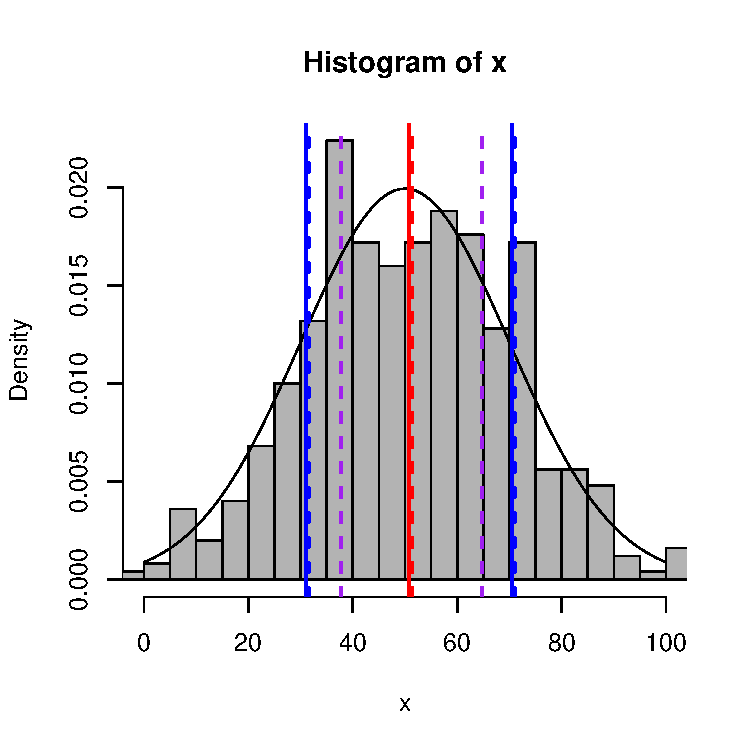
\includegraphics[width=1.1\linewidth]{figure/unnamed-chunk-11-1} 

\end{knitrout}

\end{columns}

\end{frame} 
%===============================================================================%

%===============================================================================%
\begin{frame}[fragile]%{Tendência Central: Distribuição Normal}

\begin{columns}[c]

\column{0.49\linewidth}

\begin{knitrout}\tiny
\definecolor{shadecolor}{rgb}{0.969, 0.969, 0.969}\color{fgcolor}\begin{kframe}
\begin{alltt}
\hlkwd{set.seed}\hlstd{(}\hlnum{1979}\hlstd{)}
\hlstd{x} \hlkwb{<-} \hlkwd{rgeom}\hlstd{(}\hlnum{500}\hlstd{,}\hlnum{0.1}\hlstd{)}

\hlkwd{mean}\hlstd{(x)}
\end{alltt}
\begin{verbatim}
## [1] 8.66
\end{verbatim}
\begin{alltt}
\hlkwd{median}\hlstd{(x)}
\end{alltt}
\begin{verbatim}
## [1] 6
\end{verbatim}
\begin{alltt}
\hlkwd{sd}\hlstd{(x)}
\end{alltt}
\begin{verbatim}
## [1] 8.846973
\end{verbatim}
\begin{alltt}
\hlkwd{quantile}\hlstd{(x,}\hlkwc{probs}\hlstd{=}\hlkwd{c}\hlstd{(}\hlnum{0.25}\hlstd{,}\hlnum{0.50}\hlstd{))}
\end{alltt}
\begin{verbatim}
## 25% 50% 
##   3   6
\end{verbatim}
\end{kframe}
\end{knitrout}

\column{0.5\linewidth}
\centering
\begin{knitrout}
\definecolor{shadecolor}{rgb}{0.969, 0.969, 0.969}\color{fgcolor}
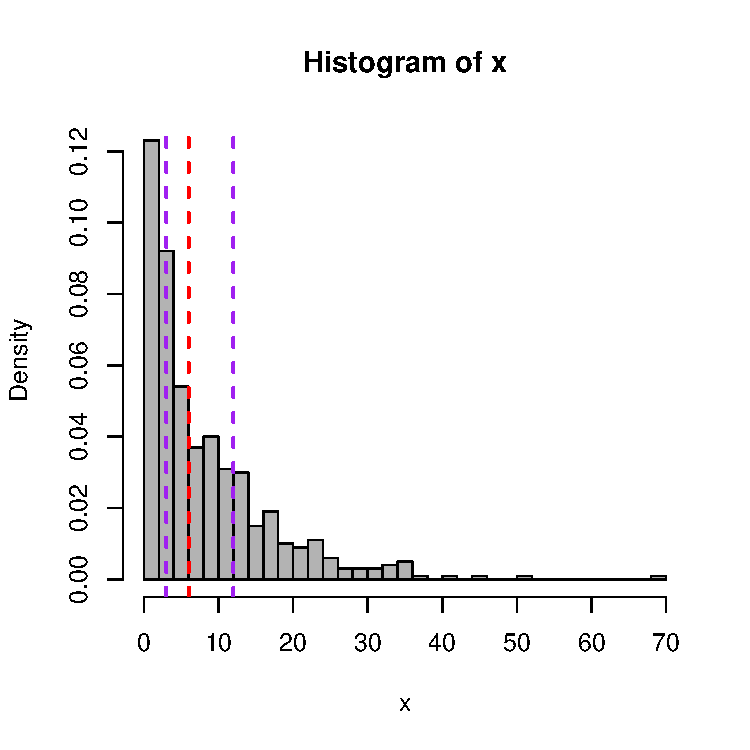
\includegraphics[width=1.1\linewidth]{figure/unnamed-chunk-13-1} 

\end{knitrout}

\end{columns}

\end{frame} 
%===============================================================================%

%===============================================================================%
\begin{frame}[fragile]%{Tendência Central: Distribuição Normal}

\begin{columns}[c]

\column{0.49\linewidth}

\begin{knitrout}\tiny
\definecolor{shadecolor}{rgb}{0.969, 0.969, 0.969}\color{fgcolor}\begin{kframe}
\begin{alltt}
\hlkwd{set.seed}\hlstd{(}\hlnum{1979}\hlstd{)}
\hlstd{x} \hlkwb{<-} \hlkwd{rgeom}\hlstd{(}\hlnum{500}\hlstd{,}\hlnum{0.1}\hlstd{)}
\hlcom{## }
\hlcom{## hist(x,breaks=30,prob=T,col='gray70')}
\hlcom{## abline(v=mean(x),col='red',lwd=2,lty=1)}
\hlcom{## abline(v=median(x),col='red',lwd=2,lty=2)}
\hlcom{## abline(v=c(mean(x)+sd(x),mean(x)-sd(x)),#}
\hlcom{##        col='blue',lwd=2,lty=1)}
\hlcom{## abline(v=quantile(x,prob=c(0.25,0.75)),#}
\hlcom{##        col='purple',lwd=2,lty=2)}
\hlcom{## abline(v=quantile(x,prob=c(0.16,0.84)),#}
\hlcom{##        col='blue',lwd=2,lty=2)}
\end{alltt}
\end{kframe}
\end{knitrout}

\column{0.5\linewidth}
\centering
\begin{knitrout}
\definecolor{shadecolor}{rgb}{0.969, 0.969, 0.969}\color{fgcolor}
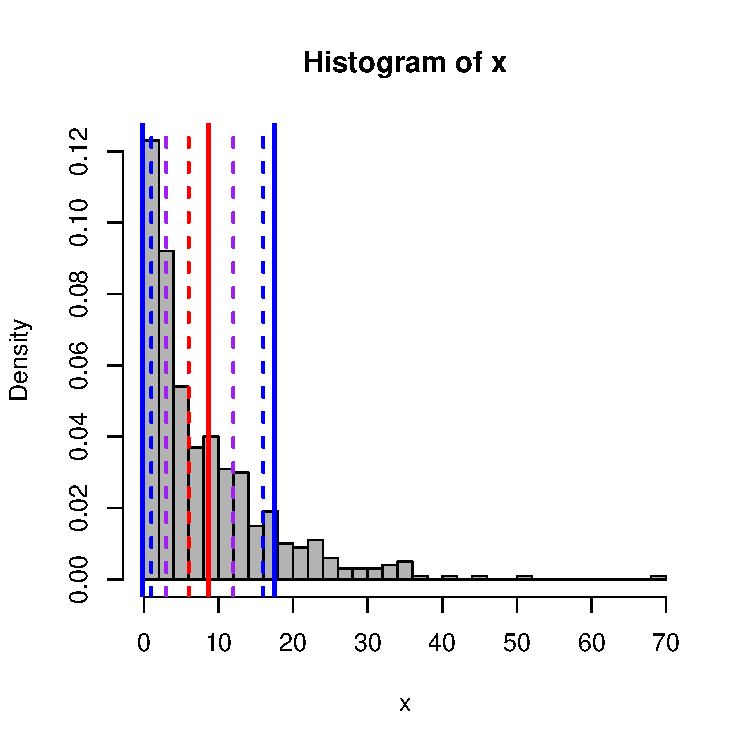
\includegraphics[width=1.1\linewidth]{figure/unnamed-chunk-15-1} 

\end{knitrout}

\end{columns}

\end{frame} 
%===============================================================================%



%===============================================================================%
\begin{frame}[fragile]%{Tendência Central: Distribuição Normal}

\begin{itemize}
  \item Os quantis são muito mais robustos com relação a valores extremos (\emph{outliers})
\end{itemize}
\begin{columns}[c]

\column{0.49\linewidth}

\begin{knitrout}\tiny
\definecolor{shadecolor}{rgb}{0.969, 0.969, 0.969}\color{fgcolor}\begin{kframe}
\begin{alltt}
\hlstd{x} \hlkwb{<-} \hlkwd{c}\hlstd{(}\hlnum{1}\hlstd{,}\hlnum{2}\hlstd{,}\hlnum{3}\hlstd{,}\hlnum{2}\hlstd{,}\hlnum{3}\hlstd{,}\hlnum{4}\hlstd{,}\hlnum{5}\hlstd{,}\hlnum{6}\hlstd{,}\hlnum{2}\hlstd{,}\hlnum{3}\hlstd{,}\hlnum{5}\hlstd{,}\hlnum{4}\hlstd{,}\hlnum{1}\hlstd{,}\hlnum{2}\hlstd{,}\hlnum{3}\hlstd{,}\hlnum{4}\hlstd{,}\hlnum{5}\hlstd{,}\hlnum{5}\hlstd{,}\hlnum{6}\hlstd{,}\hlnum{30}\hlstd{)}

\hlkwd{mean}\hlstd{(x)}
\end{alltt}
\begin{verbatim}
## [1] 4.8
\end{verbatim}
\begin{alltt}
\hlkwd{median}\hlstd{(x)}
\end{alltt}
\begin{verbatim}
## [1] 3.5
\end{verbatim}
\begin{alltt}
\hlkwd{hist}\hlstd{(x,}\hlkwc{breaks}\hlstd{=}\hlnum{40}\hlstd{,}\hlkwc{prob}\hlstd{=T,,}\hlkwc{col}\hlstd{=}\hlstr{'gray70'}\hlstd{)}
\hlkwd{abline}\hlstd{(}\hlkwc{v}\hlstd{=}\hlkwd{mean}\hlstd{(x),}\hlkwc{col}\hlstd{=}\hlstr{'red'}\hlstd{,}\hlkwc{lwd}\hlstd{=}\hlnum{2}\hlstd{,}\hlkwc{lty}\hlstd{=}\hlnum{1}\hlstd{)}
\hlkwd{abline}\hlstd{(}\hlkwc{v}\hlstd{=}\hlkwd{median}\hlstd{(x),}\hlkwc{col}\hlstd{=}\hlstr{'red'}\hlstd{,}\hlkwc{lwd}\hlstd{=}\hlnum{2}\hlstd{,}\hlkwc{lty}\hlstd{=}\hlnum{2}\hlstd{)}
\end{alltt}
\end{kframe}
\end{knitrout}

\column{0.5\linewidth}
\centering
\begin{knitrout}
\definecolor{shadecolor}{rgb}{0.969, 0.969, 0.969}\color{fgcolor}
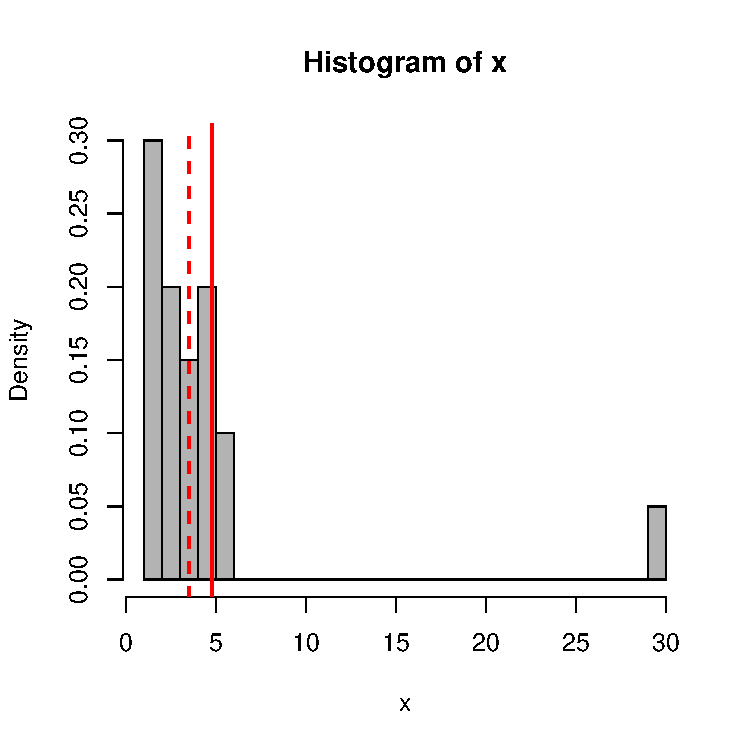
\includegraphics[width=1.1\linewidth]{figure/unnamed-chunk-17-1} 

\end{knitrout}

\end{columns}

\end{frame} 
%===============================================================================%


%===============================================================================%
\begin{frame}[fragile]%{Tendência Central: Distribuição Normal}

\begin{itemize}
  \item Os quantis são muito mais robustos com relação a valores extremos (\emph{outliers})
\end{itemize}
\begin{columns}[c]

\column{0.49\linewidth}

\begin{knitrout}\tiny
\definecolor{shadecolor}{rgb}{0.969, 0.969, 0.969}\color{fgcolor}\begin{kframe}
\begin{alltt}
\hlstd{x} \hlkwb{<-} \hlkwd{c}\hlstd{(}\hlnum{1}\hlstd{,}\hlnum{2}\hlstd{,}\hlnum{3}\hlstd{,}\hlnum{2}\hlstd{,}\hlnum{3}\hlstd{,}\hlnum{4}\hlstd{,}\hlnum{5}\hlstd{,}\hlnum{6}\hlstd{,}\hlnum{2}\hlstd{,}\hlnum{3}\hlstd{,}\hlnum{5}\hlstd{,}\hlnum{4}\hlstd{,}\hlnum{1}\hlstd{,}\hlnum{2}\hlstd{,}\hlnum{3}\hlstd{,}\hlnum{4}\hlstd{,}\hlnum{5}\hlstd{,}\hlnum{5}\hlstd{,}\hlnum{6}\hlstd{,}\hlnum{300}\hlstd{)}

\hlkwd{mean}\hlstd{(x)}
\end{alltt}
\begin{verbatim}
## [1] 18.3
\end{verbatim}
\begin{alltt}
\hlkwd{median}\hlstd{(x)}
\end{alltt}
\begin{verbatim}
## [1] 3.5
\end{verbatim}
\begin{alltt}
\hlkwd{hist}\hlstd{(x,}\hlkwc{breaks}\hlstd{=}\hlnum{80}\hlstd{,}\hlkwc{prob}\hlstd{=T,,}\hlkwc{col}\hlstd{=}\hlstr{'gray70'}\hlstd{)}
\hlkwd{abline}\hlstd{(}\hlkwc{v}\hlstd{=}\hlkwd{mean}\hlstd{(x),}\hlkwc{col}\hlstd{=}\hlstr{'red'}\hlstd{,}\hlkwc{lwd}\hlstd{=}\hlnum{2}\hlstd{,}\hlkwc{lty}\hlstd{=}\hlnum{1}\hlstd{)}
\hlkwd{abline}\hlstd{(}\hlkwc{v}\hlstd{=}\hlkwd{median}\hlstd{(x),}\hlkwc{col}\hlstd{=}\hlstr{'red'}\hlstd{,}\hlkwc{lwd}\hlstd{=}\hlnum{2}\hlstd{,}\hlkwc{lty}\hlstd{=}\hlnum{2}\hlstd{)}
\end{alltt}
\end{kframe}
\end{knitrout}

\column{0.5\linewidth}
\centering
\begin{knitrout}
\definecolor{shadecolor}{rgb}{0.969, 0.969, 0.969}\color{fgcolor}
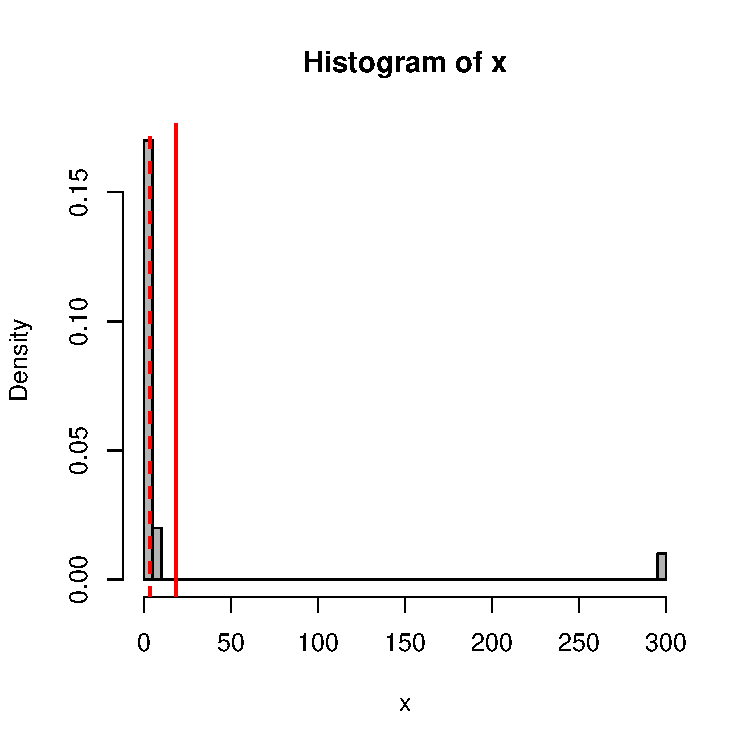
\includegraphics[width=1.1\linewidth]{figure/unnamed-chunk-19-1} 

\end{knitrout}

\end{columns}

\end{frame} 
%===============================================================================%



%===============================================================================%
\begin{frame}[fragile]%{Tendência Central: Distribuição Normal}

\begin{itemize}
  \item Os quantis são muito mais robustos com relação a valores extremos (\emph{outliers})
\end{itemize}
\begin{columns}[c]

\column{0.49\linewidth}

\begin{knitrout}\tiny
\definecolor{shadecolor}{rgb}{0.969, 0.969, 0.969}\color{fgcolor}\begin{kframe}
\begin{alltt}
\hlstd{x} \hlkwb{<-} \hlkwd{c}\hlstd{(}\hlnum{1}\hlstd{,}\hlnum{2}\hlstd{,}\hlnum{3}\hlstd{,}\hlnum{2}\hlstd{,}\hlnum{3}\hlstd{,}\hlnum{4}\hlstd{,}\hlnum{5}\hlstd{,}\hlnum{6}\hlstd{,}\hlnum{2}\hlstd{,}\hlnum{3}\hlstd{,}\hlnum{5}\hlstd{,}\hlnum{4}\hlstd{,}\hlnum{1}\hlstd{,}\hlnum{2}\hlstd{,}\hlnum{3}\hlstd{,}\hlnum{4}\hlstd{,}\hlnum{5}\hlstd{,}\hlnum{5}\hlstd{,}\hlnum{6}\hlstd{,}\hlnum{30}\hlstd{)}

\hlkwd{sd}\hlstd{(x)}
\end{alltt}
\begin{verbatim}
## [1] 6.126732
\end{verbatim}
\begin{alltt}
\hlkwd{quantile}\hlstd{(x,}\hlkwc{prob}\hlstd{=}\hlkwd{c}\hlstd{(}\hlnum{0.16}\hlstd{,}\hlnum{0.84}\hlstd{))}
\end{alltt}
\begin{verbatim}
## 16% 84% 
##   2   5
\end{verbatim}
\begin{alltt}
\hlkwd{hist}\hlstd{(x,}\hlkwc{breaks}\hlstd{=}\hlnum{40}\hlstd{,}\hlkwc{prob}\hlstd{=T,,}\hlkwc{col}\hlstd{=}\hlstr{'gray70'}\hlstd{)}
\hlkwd{abline}\hlstd{(}\hlkwc{v}\hlstd{=}\hlkwd{mean}\hlstd{(x),}\hlkwc{col}\hlstd{=}\hlstr{'red'}\hlstd{,}\hlkwc{lwd}\hlstd{=}\hlnum{2}\hlstd{,}\hlkwc{lty}\hlstd{=}\hlnum{1}\hlstd{)}
\hlkwd{abline}\hlstd{(}\hlkwc{v}\hlstd{=}\hlkwd{median}\hlstd{(x),}\hlkwc{col}\hlstd{=}\hlstr{'red'}\hlstd{,}\hlkwc{lwd}\hlstd{=}\hlnum{2}\hlstd{,}\hlkwc{lty}\hlstd{=}\hlnum{2}\hlstd{)}
\hlkwd{abline}\hlstd{(}\hlkwc{v}\hlstd{=}\hlkwd{c}\hlstd{(}\hlkwd{mean}\hlstd{(x)}\hlopt{-}\hlkwd{sd}\hlstd{(x),}\hlkwd{mean}\hlstd{(x)}\hlopt{+}\hlkwd{sd}\hlstd{(x)),}\hlcom{#}
       \hlkwc{col}\hlstd{=}\hlstr{'blue'}\hlstd{,}\hlkwc{lwd}\hlstd{=}\hlnum{2}\hlstd{,}\hlkwc{lty}\hlstd{=}\hlnum{1}\hlstd{)}
\hlkwd{abline}\hlstd{(}\hlkwc{v}\hlstd{=}\hlkwd{quantile}\hlstd{(x,}\hlkwc{prob}\hlstd{=}\hlkwd{c}\hlstd{(}\hlnum{0.16}\hlstd{,}\hlnum{0.84}\hlstd{)),}\hlcom{#}
       \hlkwc{col}\hlstd{=}\hlstr{'blue'}\hlstd{,}\hlkwc{lwd}\hlstd{=}\hlnum{2}\hlstd{,}\hlkwc{lty}\hlstd{=}\hlnum{2}\hlstd{)}
\end{alltt}
\end{kframe}
\end{knitrout}

\column{0.5\linewidth}
\centering
\begin{knitrout}
\definecolor{shadecolor}{rgb}{0.969, 0.969, 0.969}\color{fgcolor}
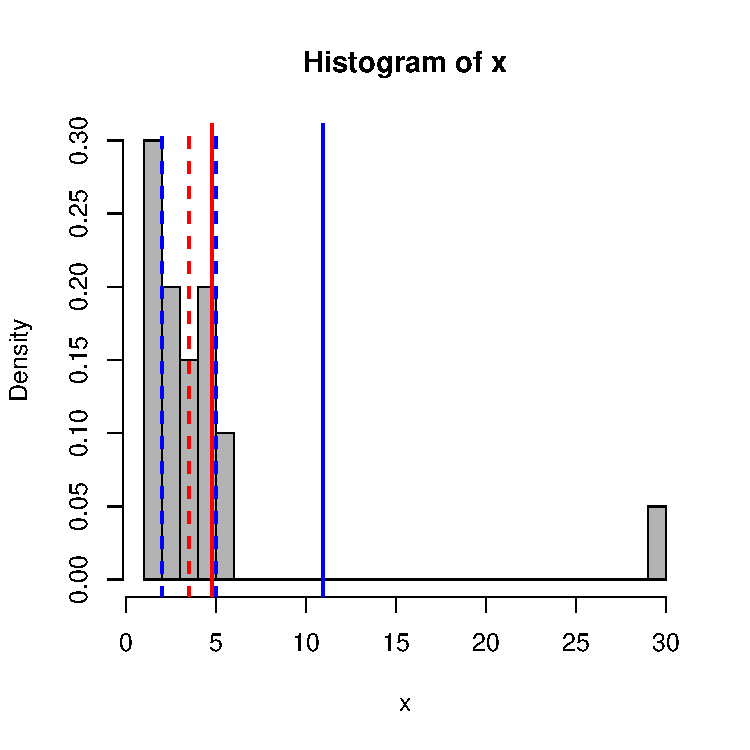
\includegraphics[width=1.1\linewidth]{figure/unnamed-chunk-21-1} 

\end{knitrout}

\end{columns}

\end{frame} 
%===============================================================================%

%===============================================================================%
\begin{frame}{Estatística Descritiva: tendência central e dispersão}
%\setbeamercovered{transparent}  
\linespread{1.5} 
 
\textbf{Tendência e dispersão para dados \emph{categóricos}?}

\begin{small}
\begin{itemize}
  \item Qual a média de (Floresta, Campo, Cidade)? \pause
  \item Solução: contagens, frequência, porcentagem, \emph{odds}\pause
  \item Exemplo: Você gosta de estatística?
\end{itemize}
\end{small}

\begin{columns}[c]
\only<4-5>{
\column{0.3\linewidth}
\begin{tiny}
\begin{table}[ht]
\centering
\begin{tabular}{rr}
  \hline
  Obs. & Gosto \\
  \hline
  1 & Sim\\
  2 & Não\\
  3 & Não\\
  4 & Não\\
  5 & Não\\
  6 & Não\\
  7 & Não\\
  8 & Sim\\
  9 & Sim\\
  \hline
\end{tabular}
\end{table}
\end{tiny}\pause
}

\column{0.6\linewidth}
\only<5>{
\begin{tiny}
\begin{table}[ht]
\centering
\begin{tabular}{rrrrr}
  \hline
  Variável & Contagem & Frequência & Porcentagem & \emph{odds}\\
  \hline
  Sim & 3 & 0.33 & 33\% & 0.5\\
  Não & 6 & 0.66 & 66\% & 2\\
  \hline
\end{tabular}
\end{table}
\end{tiny}\pause
}
\end{columns}
\end{frame} 
%===============================================================================%

%===============================================================================%
\begin{frame}{Estatística Descritiva: tendência central e dispersão}
%\setbeamercovered{transparent}  
\linespread{1.5} 
 
\textbf{Tendência e dispersão para dados \emph{categóricos}?}

\begin{small}
\begin{itemize}
  \item Exemplo: O quanto você gosta de estatística? (1-Abomino, 2-Odeio, 3-Não Gosto, 4-Tolero,5-Adoro)
\end{itemize}
\end{small}

\begin{columns}[c]
\column{0.3\linewidth}
\begin{tiny}
\begin{table}[ht]
\centering
\begin{tabular}{rr}
  \hline
  Obs. & Gosto \\
  \hline
  1 & 5\\
  2 & 1\\
  3 & 1\\
  4 & 1\\
  5 & 2\\
  6 & 2\\
  7 & 3\\
  8 & 3\\
  9 & 4\\
  \hline
\end{tabular}
\end{table}
\end{tiny}


\column{0.6\linewidth}
\begin{tiny}
\begin{table}[ht]
\centering
\begin{tabular}{rrrrr}
  \hline
  Variável & Contagem & Frequência & Porcentagem & \emph{odds}\\
  \hline
  Abomino & 3 & 0.33 & 33\% & 0.5\\
  Odeio & 2 & 0.25 & 25\% & 0.29\\
  Não Gosto & 2 & 0.25 & 25\% & 0.29\\
  Tolero & 1 & 0.1 & 10\% & 0.125\\
  Adoro & 1 & 0.1 & 10\% & 0.125\\
  \hline
\end{tabular}
\end{table}
\end{tiny}
\end{columns}
\end{frame} 
%===============================================================================%


\section{Análise Gráfica}


%===============================================================================%
\begin{frame}{Análise Gráfica}
\setbeamercovered{transparent}
  
\begin{itemize}

\item O ser humano tem uma capacidade incrível de processar informações visuais \pause
\vfill
\item	A análise gráfica pode ser considerada uma das partes mais importantes do processo \pause
\vfill
\item	Muitas questões podem ser respondidas sem a necessidade de (\emph{mindless}) testes  \pause
\vfill
\item  Métodos de visualição tem sido um \emph{hot topic} em análise de dados atualmente  

\end{itemize}


\end{frame} 
%===============================================================================%


%===============================================================================%
\begin{frame}{Tipos de Gráficos - 1 variável: Histograma}
  
\textbf{Histograma}  

\begin{itemize}
  \item Adequado para mostrar distribuições, pode ser usado tanto para dados categóricos quanto contínuos \pause
  \vfill
  \item  É importante definirem-se bem as subdivisões (\emph{bins})
\end{itemize}


\end{frame} 
%===============================================================================%


%===============================================================================%
\begin{frame}[fragile]{Tipos de Gráficos - 1 variável: Histograma}

\begin{columns}[t]

\column{0.56\linewidth}
\begin{knitrout}\tiny
\definecolor{shadecolor}{rgb}{0.969, 0.969, 0.969}\color{fgcolor}\begin{kframe}
\begin{alltt}
\hlkwd{hist}\hlstd{(plot.data}\hlopt{$}\hlstd{sigma0)}
\end{alltt}
\end{kframe}
\end{knitrout}

\column{0.5\linewidth}

\begin{knitrout}
\definecolor{shadecolor}{rgb}{0.969, 0.969, 0.969}\color{fgcolor}
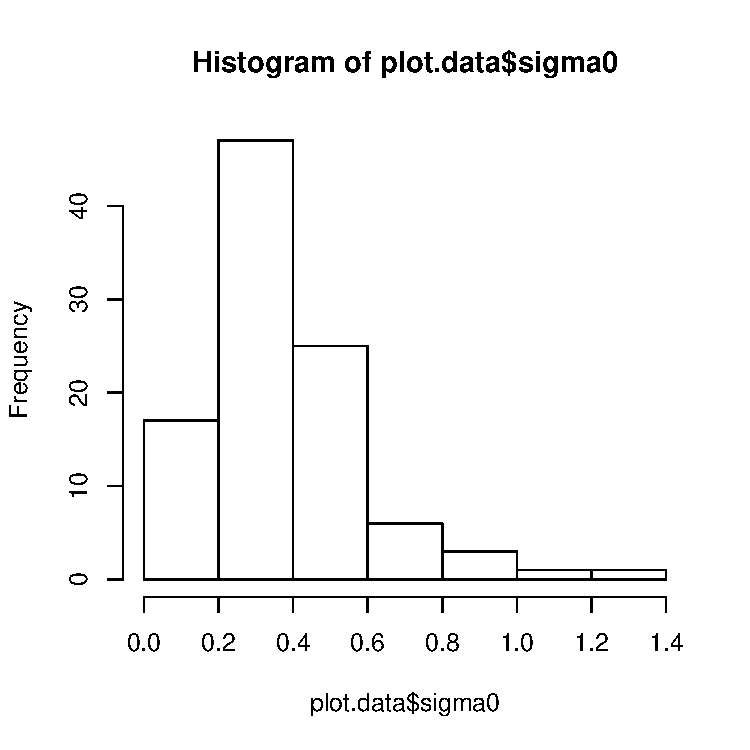
\includegraphics[width=1\linewidth]{figure/unnamed-chunk-23-1} 

\end{knitrout}

\end{columns}

\end{frame}
%===============================================================================%

%===============================================================================%
\begin{frame}[fragile]{Tipos de Gráficos - 1 variável: Histograma}
\begin{columns}[t]

\column{0.56\linewidth}
\begin{knitrout}\tiny
\definecolor{shadecolor}{rgb}{0.969, 0.969, 0.969}\color{fgcolor}\begin{kframe}
\begin{alltt}
\hlkwd{hist}\hlstd{(plot.data}\hlopt{$}\hlstd{sigma0)}
\hlkwd{hist}\hlstd{(plot.data}\hlopt{$}\hlstd{sigma0,}\hlkwc{breaks}\hlstd{=}\hlnum{40}\hlstd{)}
\end{alltt}
\end{kframe}
\end{knitrout}

\column{0.5\linewidth}

\begin{knitrout}
\definecolor{shadecolor}{rgb}{0.969, 0.969, 0.969}\color{fgcolor}
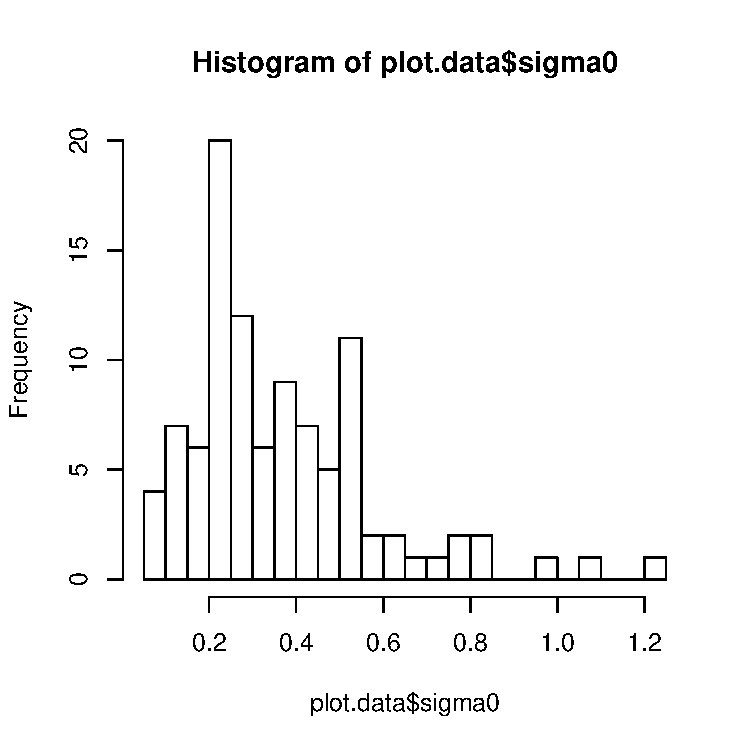
\includegraphics[width=1\linewidth]{figure/unnamed-chunk-25-1} 

\end{knitrout}

\end{columns}

\end{frame}
%===============================================================================%


%===============================================================================%
\begin{frame}[fragile]{Tipos de Gráficos - 1 variável: Histograma}

\begin{columns}[t]

\column{0.56\linewidth}
\begin{knitrout}\tiny
\definecolor{shadecolor}{rgb}{0.969, 0.969, 0.969}\color{fgcolor}\begin{kframe}
\begin{alltt}
\hlkwd{hist}\hlstd{(plot.data}\hlopt{$}\hlstd{sigma0,}\hlkwc{breaks}\hlstd{=}\hlnum{40}\hlstd{)}
\hlkwd{hist}\hlstd{(plot.data}\hlopt{$}\hlstd{sigma0,}\hlkwc{breaks}\hlstd{=}\hlnum{100}\hlstd{)}
\end{alltt}
\end{kframe}
\end{knitrout}

\column{0.5\linewidth}

\begin{knitrout}
\definecolor{shadecolor}{rgb}{0.969, 0.969, 0.969}\color{fgcolor}
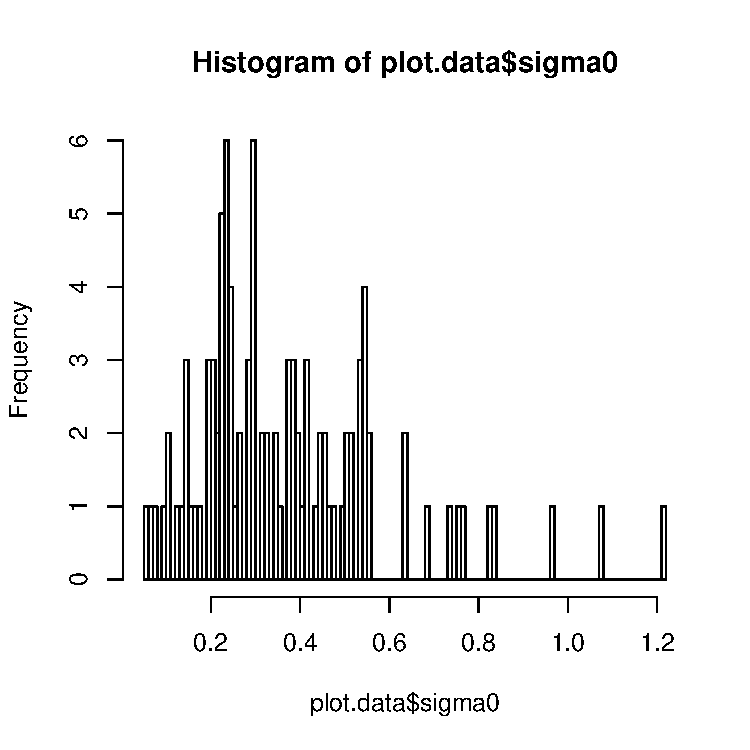
\includegraphics[width=1\linewidth]{figure/unnamed-chunk-27-1} 

\end{knitrout}

\end{columns}

\end{frame}
%===============================================================================%




%===============================================================================%
\begin{frame}[fragile]{Tipos de Gráficos - 1 variável: Histograma}

\begin{columns}[t]

\column{0.56\linewidth}
\begin{knitrout}\tiny
\definecolor{shadecolor}{rgb}{0.969, 0.969, 0.969}\color{fgcolor}\begin{kframe}
\begin{alltt}
\hlkwd{hist}\hlstd{(plot.data}\hlopt{$}\hlstd{sigma0)}
\hlkwd{hist}\hlstd{(plot.data}\hlopt{$}\hlstd{sigma0,}\hlkwc{breaks}\hlstd{=}\hlnum{40}\hlstd{)}
\hlkwd{hist}\hlstd{(}\hlnum{10}\hlopt{*}\hlkwd{log10}\hlstd{(plot.data}\hlopt{$}\hlstd{sigma0),}\hlkwc{breaks}\hlstd{=}\hlnum{30}\hlstd{)}
\end{alltt}
\end{kframe}
\end{knitrout}

\column{0.5\linewidth}

\begin{knitrout}
\definecolor{shadecolor}{rgb}{0.969, 0.969, 0.969}\color{fgcolor}
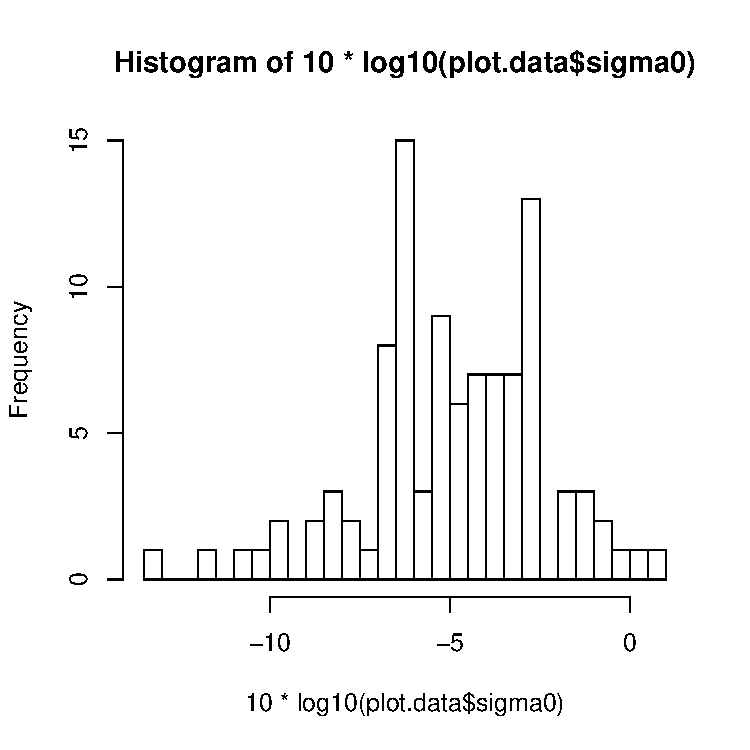
\includegraphics[width=1\linewidth]{figure/unnamed-chunk-29-1} 

\end{knitrout}

\end{columns}

\end{frame}
%===============================================================================%


%===============================================================================%
\begin{frame}[fragile]{Tipos de Gráficos - 1 variável: Histograma}

\begin{columns}[t]

\column{0.56\linewidth}
\begin{knitrout}\tiny
\definecolor{shadecolor}{rgb}{0.969, 0.969, 0.969}\color{fgcolor}\begin{kframe}
\begin{alltt}
\hlkwd{hist}\hlstd{(plot.data}\hlopt{$}\hlstd{sigma0)}
\hlkwd{hist}\hlstd{(plot.data}\hlopt{$}\hlstd{sigma0,}\hlkwc{breaks}\hlstd{=}\hlnum{40}\hlstd{)}
\hlkwd{hist}\hlstd{(plot.data}\hlopt{$}\hlstd{sigma0,}\hlkwc{breaks}\hlstd{=}\hlnum{400}\hlstd{)}
\hlkwd{hist}\hlstd{(}\hlnum{10}\hlopt{*}\hlkwd{log10}\hlstd{(plot.data}\hlopt{$}\hlstd{sigma0),}\hlkwc{breaks}\hlstd{=}\hlnum{30}\hlstd{)}
\hlkwd{hist}\hlstd{(}\hlnum{10}\hlopt{*}\hlkwd{log10}\hlstd{(plot.data}\hlopt{$}\hlstd{sigma0),}\hlkwc{breaks}\hlstd{=}\hlnum{30}\hlstd{,}\hlkwc{prob}\hlstd{=T)}
\end{alltt}
\end{kframe}
\end{knitrout}

\column{0.5\linewidth}

\begin{knitrout}
\definecolor{shadecolor}{rgb}{0.969, 0.969, 0.969}\color{fgcolor}
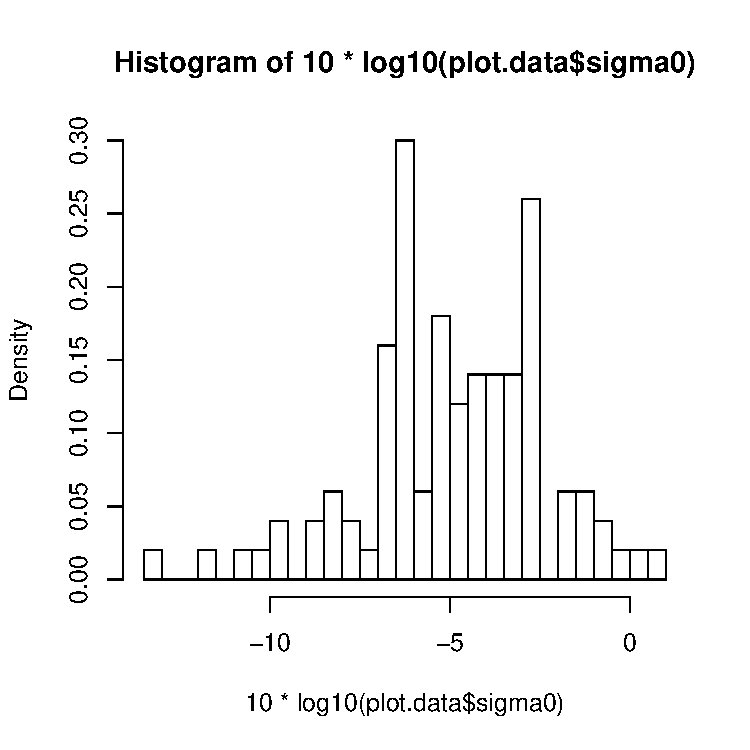
\includegraphics[width=1\linewidth]{figure/unnamed-chunk-31-1} 

\end{knitrout}

\end{columns}

\end{frame}
%===============================================================================%


%===============================================================================%
\begin{frame}[fragile]{Tipos de Gráficos - 1 variável: Histograma}

\begin{columns}[t]

\column{0.56\linewidth}
\begin{knitrout}\tiny
\definecolor{shadecolor}{rgb}{0.969, 0.969, 0.969}\color{fgcolor}\begin{kframe}
\begin{alltt}
\hlkwd{hist}\hlstd{(plot.data}\hlopt{$}\hlstd{sigma0)}
\hlkwd{hist}\hlstd{(plot.data}\hlopt{$}\hlstd{sigma0,}\hlkwc{breaks}\hlstd{=}\hlnum{40}\hlstd{)}
\hlkwd{hist}\hlstd{(plot.data}\hlopt{$}\hlstd{sigma0,}\hlkwc{breaks}\hlstd{=}\hlnum{400}\hlstd{)}
\hlkwd{hist}\hlstd{(}\hlnum{10}\hlopt{*}\hlkwd{log10}\hlstd{(plot.data}\hlopt{$}\hlstd{sigma0),}\hlkwc{breaks}\hlstd{=}\hlnum{30}\hlstd{)}
\hlkwd{hist}\hlstd{(}\hlnum{10}\hlopt{*}\hlkwd{log10}\hlstd{(plot.data}\hlopt{$}\hlstd{sigma0),}\hlkwc{breaks}\hlstd{=}\hlnum{30}\hlstd{,}\hlkwc{prob}\hlstd{=T)}
\hlkwd{hist}\hlstd{(}\hlnum{10}\hlopt{*}\hlkwd{log10}\hlstd{(plot.data}\hlopt{$}\hlstd{sigma0),}\hlkwc{breaks}\hlstd{=}\hlnum{30}\hlstd{,}\hlkwc{prob}\hlstd{=T,} \hlcom{#}
     \hlkwc{col}\hlstd{=}\hlstr{'gray70'}\hlstd{,}\hlkwc{xlab}\hlstd{=}\hlstr{"Retroespalhamento"}\hlstd{,}\hlcom{#}
     \hlkwc{ylab}\hlstd{=}\hlstr{"densidade"}\hlstd{,}\hlkwc{main}\hlstd{=}\hlnum{NA}\hlstd{)}
\end{alltt}
\end{kframe}
\end{knitrout}

\column{0.5\linewidth}

\begin{knitrout}
\definecolor{shadecolor}{rgb}{0.969, 0.969, 0.969}\color{fgcolor}
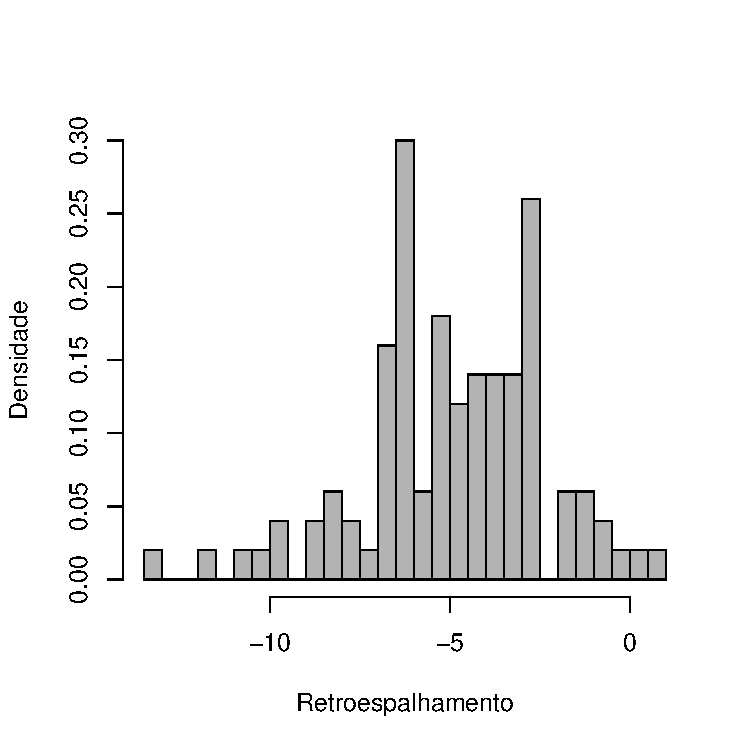
\includegraphics[width=1\linewidth]{figure/unnamed-chunk-33-1} 

\end{knitrout}

\end{columns}

\end{frame}
%===============================================================================%



%===============================================================================%
\begin{frame}{Tipos de Gráficos - 1 variável: Dot Plot}

\textbf{Dot Plot}

\begin{itemize}
  \item Similar ao histograma, mas mostra todos as observações \pause
  \vfill
  \item  Para amostras com poucas observações, ou se a escolha dos \emph{bins} não for adequada, o histograma pode distorcer a forma real da distribuição
\end{itemize}


\end{frame} 
%===============================================================================%


%===============================================================================%
\begin{frame}[fragile]{Tipos de Gráficos - 1 variável: Dot Plot}

\begin{columns}[t]

\column{0.56\linewidth}
\begin{knitrout}\tiny
\definecolor{shadecolor}{rgb}{0.969, 0.969, 0.969}\color{fgcolor}\begin{kframe}
\begin{alltt}
\hlkwd{stripchart}\hlstd{(plot.data}\hlopt{$}\hlstd{sigma0,} \hlkwc{method} \hlstd{=} \hlstr{"stack"}\hlstd{,} \hlkwc{offset} \hlstd{=} \hlnum{.5}\hlstd{,} \hlkwc{at} \hlstd{=} \hlnum{.15}\hlstd{,} \hlkwc{pch} \hlstd{=} \hlnum{19}\hlstd{)}
\end{alltt}
\end{kframe}
\end{knitrout}

\column{0.5\linewidth}

\begin{knitrout}
\definecolor{shadecolor}{rgb}{0.969, 0.969, 0.969}\color{fgcolor}
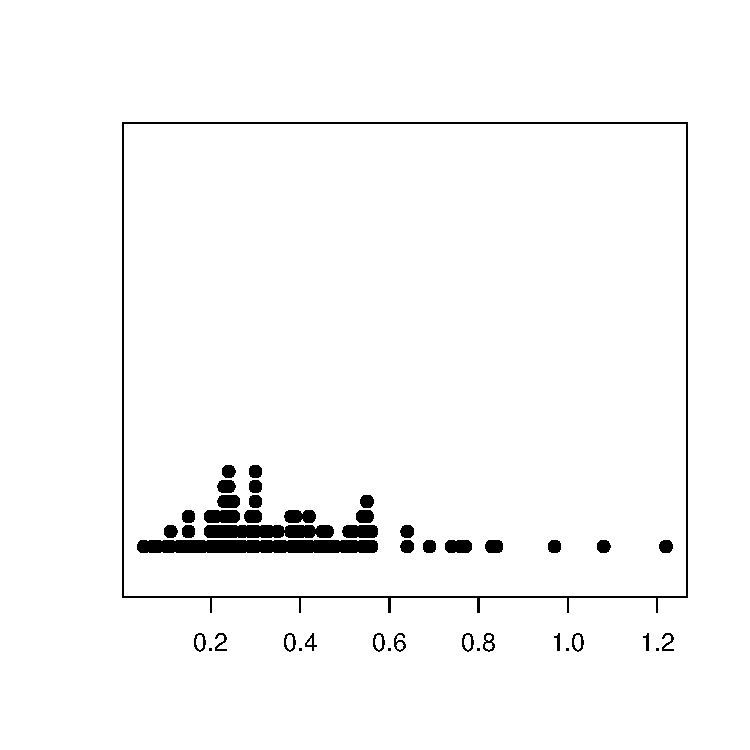
\includegraphics[width=1\linewidth]{figure/unnamed-chunk-35-1} 

\end{knitrout}

\end{columns}

\end{frame}
%===============================================================================%

%===============================================================================%
\begin{frame}{Tipos de Gráficos - 1 variável:Densidade \emph{kernel}}

\textbf{Densidade \emph{Kernel}}

\begin{itemize}
  \item Similar ao histograma, mas ajusta uma linha suavizada à distribuição \pause
  \vfill
  \item  Assim como o histograma depende das subdivisões, este gráfico depende da largura do \emmh{kernel (bandwidth)} \pause
\end{itemize}


\end{frame} 
%===============================================================================%

%===============================================================================%
\begin{frame}[fragile]{Tipos de Gráficos - 1 variável:Densidade \emph{kernel}}

\begin{columns}[t]

\column{0.56\linewidth}
\begin{knitrout}\tiny
\definecolor{shadecolor}{rgb}{0.969, 0.969, 0.969}\color{fgcolor}\begin{kframe}
\begin{alltt}
\hlkwd{plot}\hlstd{(}\hlkwd{density}\hlstd{(plot.data}\hlopt{$}\hlstd{sigma0))}
\end{alltt}
\end{kframe}
\end{knitrout}

\column{0.5\linewidth}

\begin{knitrout}
\definecolor{shadecolor}{rgb}{0.969, 0.969, 0.969}\color{fgcolor}
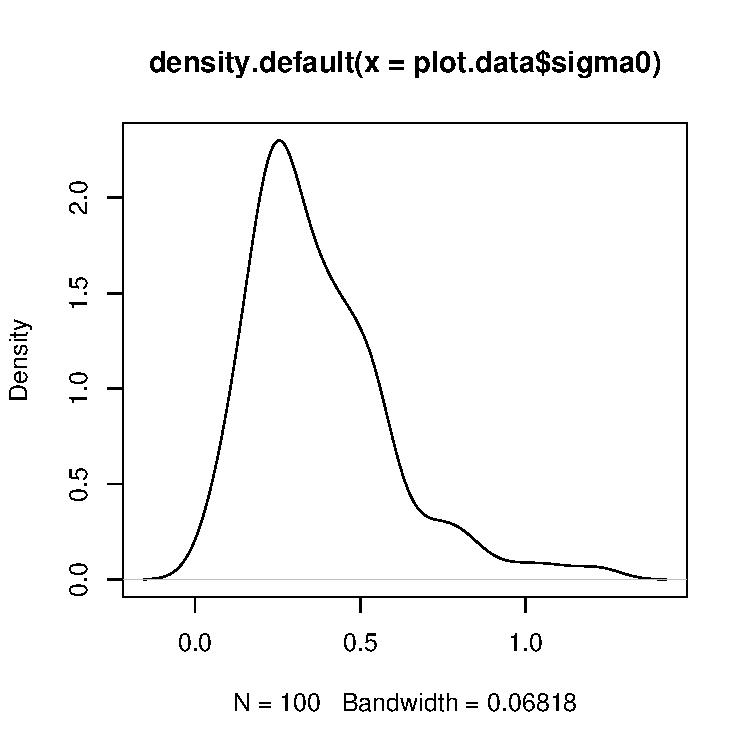
\includegraphics[width=1\linewidth]{figure/unnamed-chunk-37-1} 

\end{knitrout}

\end{columns}

\end{frame}
%===============================================================================%


%===============================================================================%
\begin{frame}[fragile]{Tipos de Gráficos - 1 variável:Densidade \emph{kernel}}

\begin{columns}[t]

\column{0.56\linewidth}
\begin{knitrout}\tiny
\definecolor{shadecolor}{rgb}{0.969, 0.969, 0.969}\color{fgcolor}\begin{kframe}
\begin{alltt}
\hlkwd{plot}\hlstd{(}\hlkwd{density}\hlstd{(plot.data}\hlopt{$}\hlstd{sigma0))}
\hlkwd{plot}\hlstd{(}\hlkwd{density}\hlstd{(plot.data}\hlopt{$}\hlstd{sigma0,} \hlkwc{bw} \hlstd{=} \hlnum{0.04}\hlstd{),}\hlkwc{main}\hlstd{=}\hlnum{NA}\hlstd{)}
\end{alltt}
\end{kframe}
\end{knitrout}

\column{0.5\linewidth}

\begin{knitrout}
\definecolor{shadecolor}{rgb}{0.969, 0.969, 0.969}\color{fgcolor}
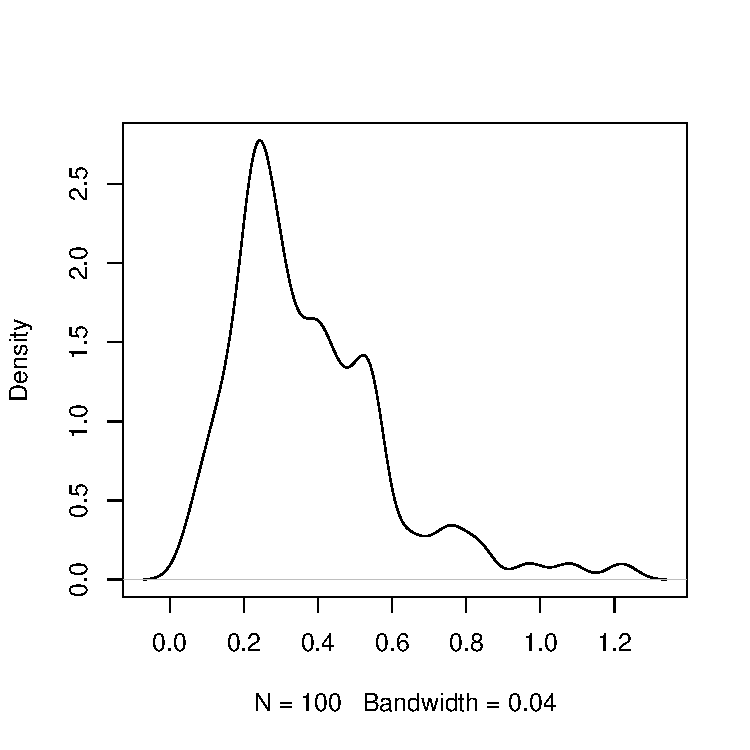
\includegraphics[width=1\linewidth]{figure/unnamed-chunk-39-1} 

\end{knitrout}

\end{columns}

\end{frame}
%===============================================================================%


%===============================================================================%
\begin{frame}[fragile]{Tipos de Gráficos - 1 variável:Densidade \emph{kernel}}

\begin{columns}[t]

\column{0.56\linewidth}
\begin{knitrout}\tiny
\definecolor{shadecolor}{rgb}{0.969, 0.969, 0.969}\color{fgcolor}\begin{kframe}
\begin{alltt}
\hlkwd{plot}\hlstd{(}\hlkwd{density}\hlstd{(plot.data}\hlopt{$}\hlstd{sigma0))}
\hlkwd{plot}\hlstd{(}\hlkwd{density}\hlstd{(plot.data}\hlopt{$}\hlstd{sigma0,} \hlkwc{bw} \hlstd{=} \hlnum{0.04}\hlstd{),}\hlkwc{main}\hlstd{=}\hlnum{NA}\hlstd{)}
\hlkwd{plot}\hlstd{(}\hlkwd{density}\hlstd{(plot.data}\hlopt{$}\hlstd{sigma0,} \hlkwc{bw} \hlstd{=} \hlnum{0.08}\hlstd{),}\hlkwc{main}\hlstd{=}\hlnum{NA}\hlstd{)}
\end{alltt}
\end{kframe}
\end{knitrout}

\column{0.5\linewidth}

\begin{knitrout}
\definecolor{shadecolor}{rgb}{0.969, 0.969, 0.969}\color{fgcolor}
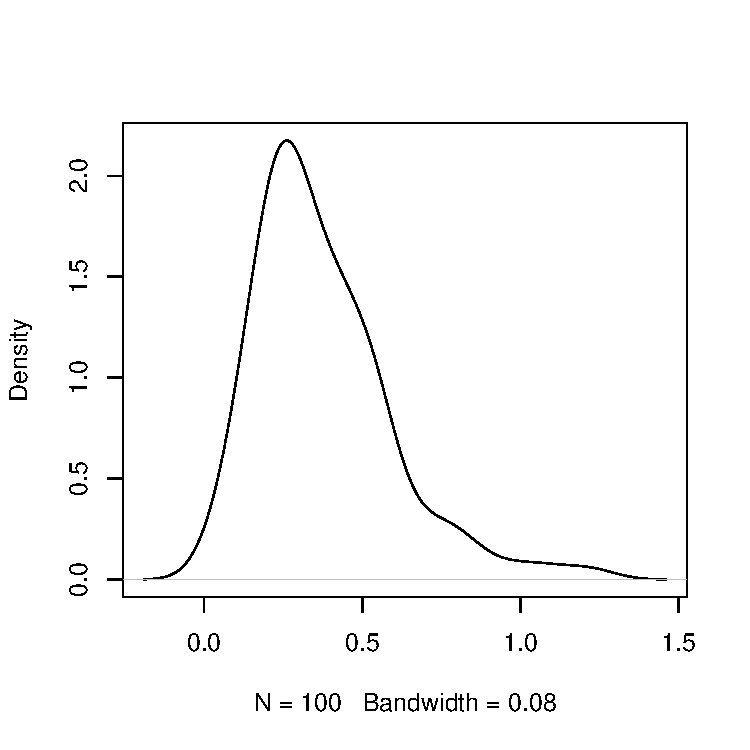
\includegraphics[width=1\linewidth]{figure/unnamed-chunk-41-1} 

\end{knitrout}

\end{columns}

\end{frame}
%===============================================================================%



%===============================================================================%
\begin{frame}[fragile]{Tipos de Gráficos - 1 variável:Densidade \emph{kernel}}

\begin{columns}[t]

\column{0.56\linewidth}
\begin{knitrout}\tiny
\definecolor{shadecolor}{rgb}{0.969, 0.969, 0.969}\color{fgcolor}\begin{kframe}
\begin{alltt}
\hlkwd{plot}\hlstd{(}\hlkwd{density}\hlstd{(plot.data}\hlopt{$}\hlstd{sigma0))}
\hlkwd{plot}\hlstd{(}\hlkwd{density}\hlstd{(plot.data}\hlopt{$}\hlstd{sigma0,} \hlkwc{bw} \hlstd{=} \hlnum{0.04}\hlstd{),}\hlkwc{main}\hlstd{=}\hlnum{NA}\hlstd{)}
\hlkwd{plot}\hlstd{(}\hlkwd{density}\hlstd{(plot.data}\hlopt{$}\hlstd{sigma0,} \hlkwc{bw} \hlstd{=} \hlnum{0.08}\hlstd{),}\hlkwc{main}\hlstd{=}\hlnum{NA}\hlstd{)}
\hlkwd{plot}\hlstd{(}\hlkwd{density}\hlstd{(}\hlnum{10}\hlopt{*}\hlkwd{log10}\hlstd{(plot.data}\hlopt{$}\hlstd{sigma0)),}\hlkwc{main}\hlstd{=}\hlnum{NA}\hlstd{)}
\end{alltt}
\end{kframe}
\end{knitrout}

\column{0.5\linewidth}

\begin{knitrout}
\definecolor{shadecolor}{rgb}{0.969, 0.969, 0.969}\color{fgcolor}
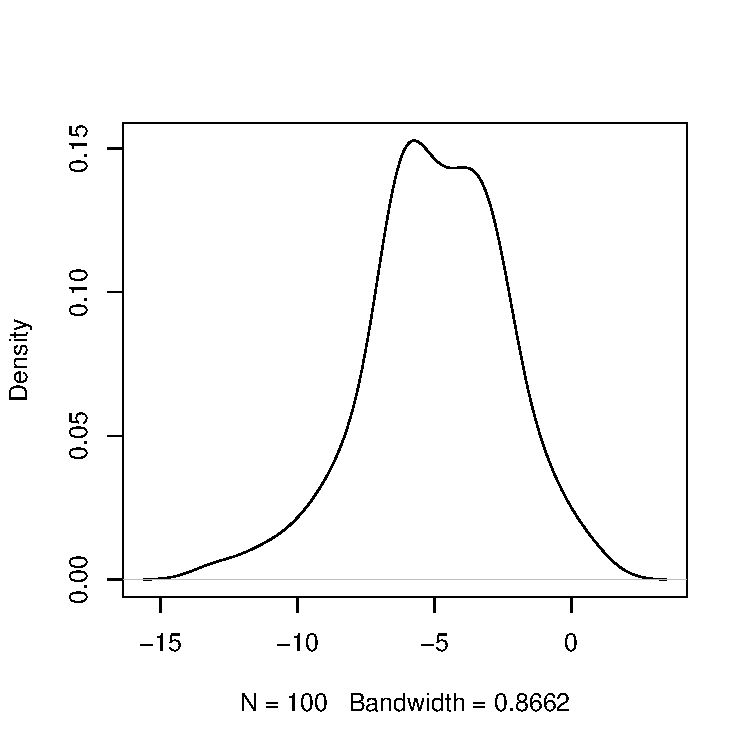
\includegraphics[width=1\linewidth]{figure/unnamed-chunk-43-1} 

\end{knitrout}

\end{columns}

\end{frame}
%===============================================================================%



%===============================================================================%
\begin{frame}[fragile]{Tipos de Gráficos - 1 variável:Densidade \emph{kernel}}

\begin{columns}[t]

\column{0.56\linewidth}
\begin{knitrout}\tiny
\definecolor{shadecolor}{rgb}{0.969, 0.969, 0.969}\color{fgcolor}\begin{kframe}
\begin{alltt}
\hlkwd{plot}\hlstd{(}\hlkwd{density}\hlstd{(plot.data}\hlopt{$}\hlstd{sigma0))}
\hlkwd{plot}\hlstd{(}\hlkwd{density}\hlstd{(plot.data}\hlopt{$}\hlstd{sigma0,} \hlkwc{bw} \hlstd{=} \hlnum{0.04}\hlstd{),}\hlkwc{main}\hlstd{=}\hlnum{NA}\hlstd{)}
\hlkwd{plot}\hlstd{(}\hlkwd{density}\hlstd{(plot.data}\hlopt{$}\hlstd{sigma0,} \hlkwc{bw} \hlstd{=} \hlnum{0.08}\hlstd{),}\hlkwc{main}\hlstd{=}\hlnum{NA}\hlstd{)}
\hlkwd{plot}\hlstd{(}\hlkwd{density}\hlstd{(}\hlnum{10}\hlopt{*}\hlkwd{log10}\hlstd{(plot.data}\hlopt{$}\hlstd{sigma0)),}\hlkwc{main}\hlstd{=}\hlnum{NA}\hlstd{)}
\hlkwd{plot}\hlstd{(}\hlkwd{density}\hlstd{(}\hlnum{10}\hlopt{*}\hlkwd{log10}\hlstd{(plot.data}\hlopt{$}\hlstd{sigma0),} \hlkwc{bw}\hlstd{=}\hlnum{1}\hlstd{),}\hlkwc{main}\hlstd{=}\hlnum{NA}\hlstd{)}
\end{alltt}
\end{kframe}
\end{knitrout}

\column{0.5\linewidth}

\begin{knitrout}
\definecolor{shadecolor}{rgb}{0.969, 0.969, 0.969}\color{fgcolor}
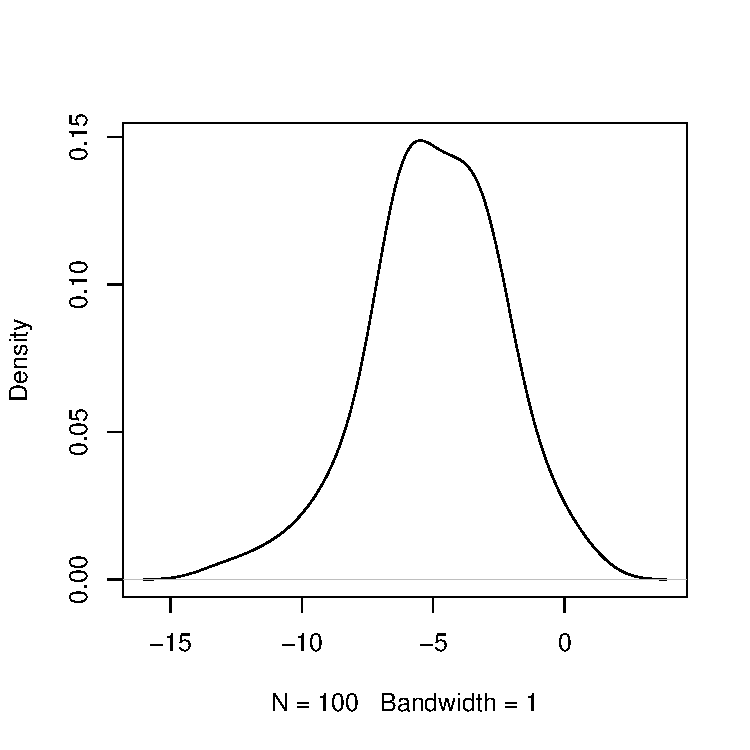
\includegraphics[width=1\linewidth]{figure/unnamed-chunk-45-1} 

\end{knitrout}

\end{columns}

\end{frame}
%===============================================================================%


%===============================================================================%
\begin{frame}{Tipos de Gráficos - 1 variável: Gráfico de Barras} 

\textbf{Gráfico de Barras}
  
\begin{itemize}
  \item Adequado para mostrar proporções, especialmente apropriado para contagens de variáveis categóricas \pause
  \vfill
  \item  Pode ser mostrado lado a lado ou empilhado \pause
  \vfill
  \item Transmite a impressão de um dado \textbf{cumulativo} \pause
  \vfill
  \item Não é recomendado para valores pontuais (ex: média)
\end{itemize}


\end{frame} 
%===============================================================================%


%===============================================================================%
\begin{frame}[fragile]{Tipos de Gráficos - 1 variável: Gráfico de Barras}

\begin{columns}[t]

\column{0.56\linewidth}
\begin{knitrout}\tiny
\definecolor{shadecolor}{rgb}{0.969, 0.969, 0.969}\color{fgcolor}\begin{kframe}
\begin{alltt}
\hlstd{stats} \hlkwb{<-} \hlkwd{factor}\hlstd{(}\hlkwd{c}\hlstd{(}\hlstr{"Sim"}\hlstd{,}\hlstr{"Não"}\hlstd{,}\hlstr{"Não"}\hlstd{,}\hlstr{"Não"}\hlstd{,}\hlstr{"Não"}\hlstd{,}
                 \hlstr{"Não"}\hlstd{,}\hlstr{"Não"}\hlstd{,}\hlstr{"Sim"}\hlstd{,}\hlstr{"Sim"}\hlstd{))}
\hlstd{summ} \hlkwb{<-} \hlkwd{table}\hlstd{(stats)}
\hlstd{summ}
\end{alltt}
\begin{verbatim}
## stats
## Não Sim 
##   6   3
\end{verbatim}
\begin{alltt}
\hlkwd{barplot}\hlstd{(summ)}
\end{alltt}
\end{kframe}
\end{knitrout}

\column{0.5\linewidth}

\begin{knitrout}
\definecolor{shadecolor}{rgb}{0.969, 0.969, 0.969}\color{fgcolor}
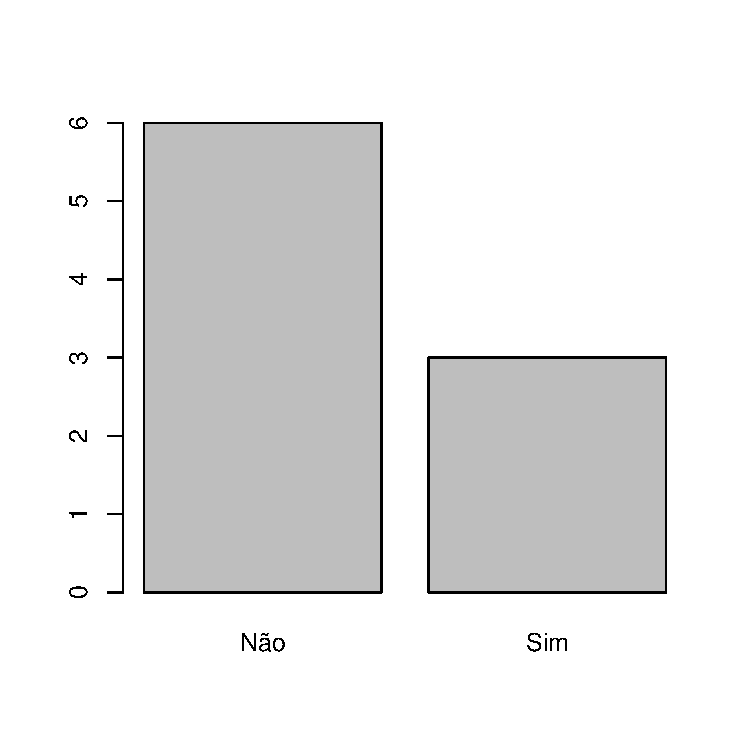
\includegraphics[width=1\linewidth]{figure/unnamed-chunk-47-1} 

\end{knitrout}

\end{columns}

\end{frame}
%===============================================================================%



%===============================================================================%
\begin{frame}[fragile]{Tipos de Gráficos - 1 variável: Gráfico de Barras}

\begin{columns}[t]

\column{0.56\linewidth}
\begin{knitrout}\tiny
\definecolor{shadecolor}{rgb}{0.969, 0.969, 0.969}\color{fgcolor}\begin{kframe}
\begin{alltt}
\hlstd{stats} \hlkwb{<-} \hlkwd{factor}\hlstd{(}\hlkwd{c}\hlstd{(}\hlstr{"Sim"}\hlstd{,}\hlstr{"Não"}\hlstd{,}\hlstr{"Não"}\hlstd{,}\hlstr{"Não"}\hlstd{,}\hlstr{"Não"}\hlstd{,}
                  \hlstr{"Não"}\hlstd{,}\hlstr{"Não"}\hlstd{,}\hlstr{"Sim"}\hlstd{,}\hlstr{"Sim"}\hlstd{))}
\hlstd{summ} \hlkwb{<-} \hlkwd{table}\hlstd{(stats)}
\hlstd{summ}
\hlkwd{barplot}\hlstd{(summ)}
\hlkwd{barplot}\hlstd{(summ,}\hlkwc{ylim}\hlstd{=}\hlkwd{c}\hlstd{(}\hlnum{0}\hlstd{,}\hlnum{10}\hlstd{))}
\end{alltt}
\end{kframe}
\end{knitrout}

\column{0.5\linewidth}

\begin{knitrout}
\definecolor{shadecolor}{rgb}{0.969, 0.969, 0.969}\color{fgcolor}
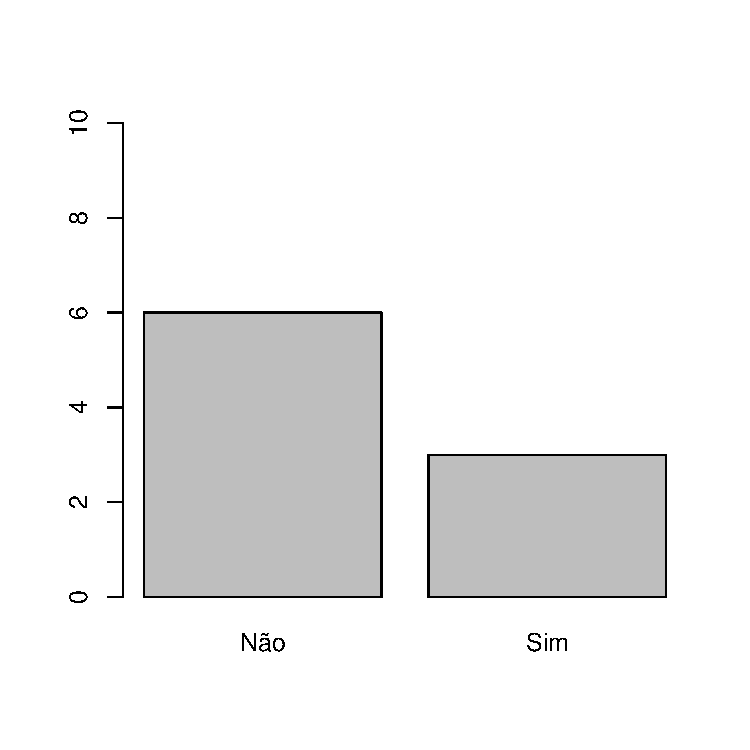
\includegraphics[width=1\linewidth]{figure/unnamed-chunk-49-1} 

\end{knitrout}

\end{columns}

\end{frame}
%===============================================================================%


%===============================================================================%
\begin{frame}[fragile]{Tipos de Gráficos - 1 variável: Gráfico de Barras} 

\begin{columns}[t]

\column{0.56\linewidth}
\begin{knitrout}\tiny
\definecolor{shadecolor}{rgb}{0.969, 0.969, 0.969}\color{fgcolor}\begin{kframe}
\begin{alltt}
\hlstd{stats} \hlkwb{<-} \hlkwd{factor}\hlstd{(}\hlkwd{c}\hlstd{(}\hlstr{"Sim"}\hlstd{,}\hlstr{"Não"}\hlstd{,}\hlstr{"Não"}\hlstd{,}\hlstr{"Não"}\hlstd{,}\hlstr{"Não"}\hlstd{,}
                  \hlstr{"Não"}\hlstd{,}\hlstr{"Não"}\hlstd{,}\hlstr{"Sim"}\hlstd{,}\hlstr{"Sim"}\hlstd{))}
\hlstd{summ} \hlkwb{<-} \hlkwd{table}\hlstd{(stats)}
\hlstd{summ}
\hlkwd{barplot}\hlstd{(summ)}
\hlkwd{barplot}\hlstd{(summ,}\hlkwc{ylim}\hlstd{=}\hlkwd{c}\hlstd{(}\hlnum{0}\hlstd{,}\hlnum{10}\hlstd{))}
\hlkwd{barplot}\hlstd{(summ,}\hlkwc{horiz}\hlstd{=T)}
\end{alltt}
\end{kframe}
\end{knitrout}

\column{0.5\linewidth}

\begin{knitrout}
\definecolor{shadecolor}{rgb}{0.969, 0.969, 0.969}\color{fgcolor}
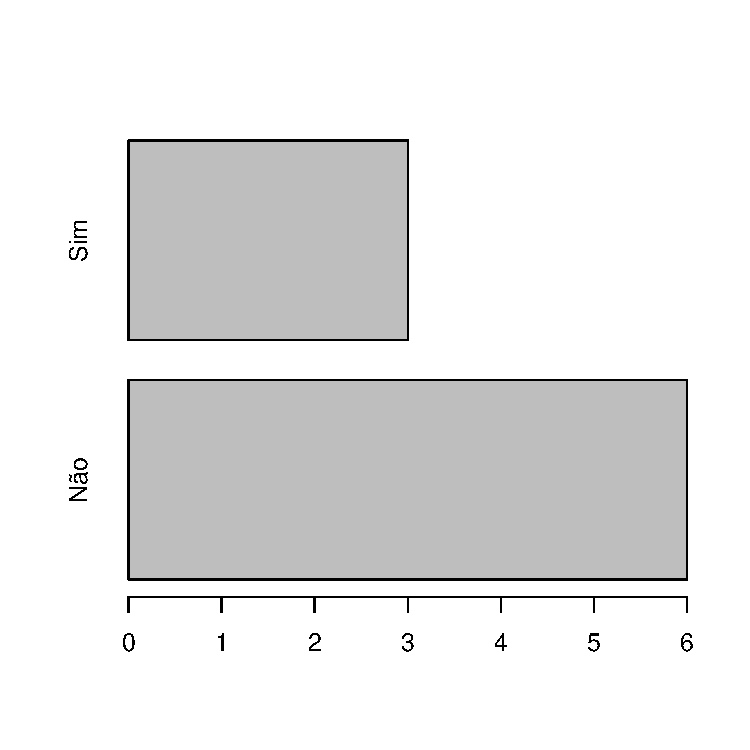
\includegraphics[width=1\linewidth]{figure/unnamed-chunk-51-1} 

\end{knitrout}

\end{columns}

\end{frame}
%===============================================================================%

%===============================================================================%
\begin{frame}[fragile]{Tipos de Gráficos - 1 variável: Gráfico de Barras} 

\begin{columns}[t]

\column{0.6\linewidth}
\begin{itemize}

\item \scriptsize{Inapropriado, pois as médias são valores pontuais, e centrais.}
\end{itemize}

\begin{knitrout}\tiny
\definecolor{shadecolor}{rgb}{0.969, 0.969, 0.969}\color{fgcolor}\begin{kframe}
\begin{alltt}
\hlkwd{barplot}\hlstd{(mean.bs,}\hlkwc{las}\hlstd{=}\hlnum{2}\hlstd{,}\hlkwc{ylab}\hlstd{=}\hlstr{"Retroespalhamento Médio"}\hlstd{)}
\end{alltt}
\end{kframe}
\end{knitrout}

\column{0.4\linewidth}

\begin{knitrout}
\definecolor{shadecolor}{rgb}{0.969, 0.969, 0.969}\color{fgcolor}
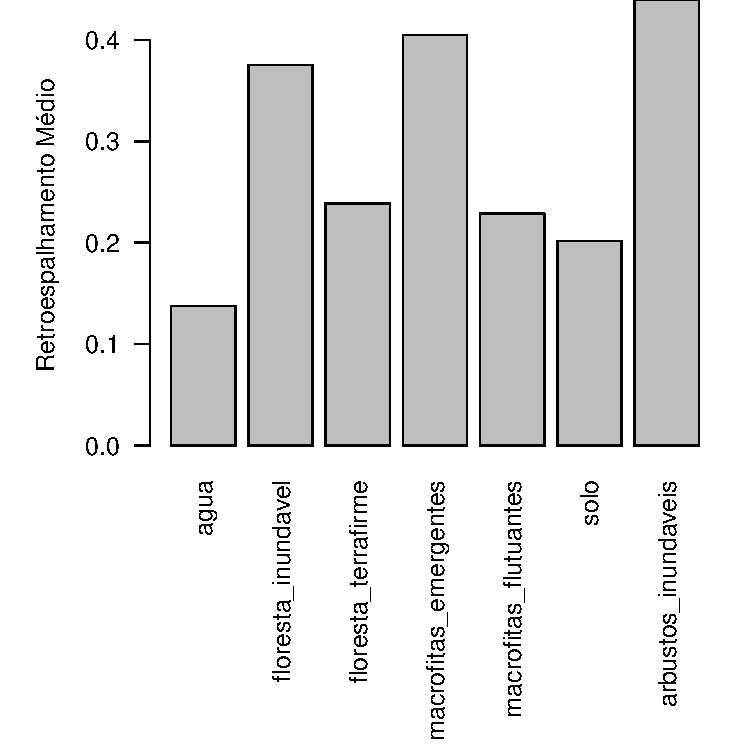
\includegraphics[width=1\linewidth]{figure/unnamed-chunk-53-1} 

\end{knitrout}

\end{columns}

\end{frame}
%===============================================================================%


%===============================================================================%
\begin{frame}[fragile]{Tipos de Gráficos - 1+ variável: Gráfico de Barras}

\begin{columns}[c]

\column{0.5\linewidth}

\begin{knitrout}\tiny
\definecolor{shadecolor}{rgb}{0.969, 0.969, 0.969}\color{fgcolor}\begin{kframe}
\begin{alltt}
\hlkwd{load}\hlstd{(}\hlstr{'rich+env_jun.Rdata'}\hlstd{)}
\hlstd{granulo} \hlkwb{<-} \hlstd{rich.env.jun[,}\hlnum{34}\hlopt{:}\hlnum{40}\hlstd{]}
\hlstd{granulo} \hlkwb{<-} \hlkwd{t}\hlstd{(}\hlkwd{as.matrix}\hlstd{(granulo))}
\hlkwd{barplot}\hlstd{(granulo,}\hlkwc{col}\hlstd{=}\hlkwd{rainbow}\hlstd{(}\hlnum{7}\hlstd{),}\hlkwc{legend}\hlstd{=T,}\hlcom{#}
    \hlkwc{args.legend} \hlstd{=} \hlkwd{list}\hlstd{(}\hlkwc{x}\hlstd{=}\hlstr{"top"}\hlstd{,} \hlkwc{inset}\hlstd{=}\hlkwd{c}\hlstd{(}\hlnum{0}\hlstd{,}\hlopt{-}\hlnum{0.7}\hlstd{),}\hlkwc{ncol}\hlstd{=}\hlnum{3}\hlstd{))}
\end{alltt}
\end{kframe}
\end{knitrout}

\column{0.5\linewidth}

\begin{knitrout}
\definecolor{shadecolor}{rgb}{0.969, 0.969, 0.969}\color{fgcolor}
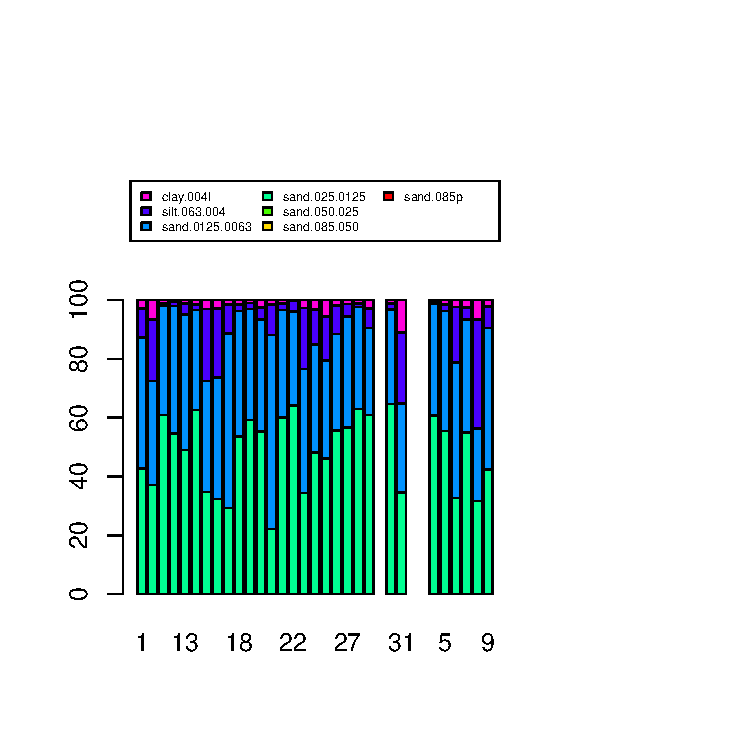
\includegraphics[width=1.4\linewidth]{figure/unnamed-chunk-55-1} 

\end{knitrout}

\end{columns}

\end{frame}
%===============================================================================%


%===============================================================================%
\begin{frame}{Tipos de Gráficos - 1 variável: Gráfico de Pizza}
  
\begin{itemize}
  \item Gráficos de pizza servem para\ldots \pause
  \vfill
  \item  \dots nada!
  \vfill
  \item Nosso cérebro é muito mais apto em julgar distâncias do que áreas ou ângulos. \pause
  \vfill
  \item A partir de hoje, podem abolir gráficos de pizza do seu repertório.
\end{itemize}

\end{frame} 
%===============================================================================%

%===============================================================================%
\begin{frame}{Tipos de Gráficos - 2 variáveis: Dispersão (\emph{scatterplot})}

\textbf{Diagrama de Dispersão (\emph{scatterplot})}

\begin{itemize}
  \item Um dos gráficos mais úteis em estatística \ldots \pause
  \vfill
  \item   Pode servir para visualizar duas variáveis contínuas, ou uma variável contínua vs. uma categórica
  \begin{itemize}
  \item Desde que a variável categórica seja codificada
  \end{itemize}
  \vfill
  \item Pode ser complementado por barras de erro \pause
  \vfill
  \item Cuidado ao unir os pontos com linhas, pois isso passa uma noção de continuidade!
\end{itemize}

\end{frame} 
%===============================================================================%


%===============================================================================%
\begin{frame}[fragile]{Tipos de Gráficos - 2 variáveis: Dispersão (\emph{scatterplot})}

\begin{columns}[t]

\column{0.6\linewidth}

\begin{knitrout}\tiny
\definecolor{shadecolor}{rgb}{0.969, 0.969, 0.969}\color{fgcolor}\begin{kframe}
\begin{alltt}
\hlkwd{plot}\hlstd{(mean.bs,}\hlkwc{las}\hlstd{=}\hlnum{2}\hlstd{,}
     \hlkwc{ylab}\hlstd{=}\hlstr{"Retroespalhamento Médio"}\hlstd{,}\hlkwc{type}\hlstd{=}\hlstr{"p"}\hlstd{)}
\end{alltt}
\end{kframe}
\end{knitrout}

\column{0.4\linewidth}

\begin{knitrout}
\definecolor{shadecolor}{rgb}{0.969, 0.969, 0.969}\color{fgcolor}
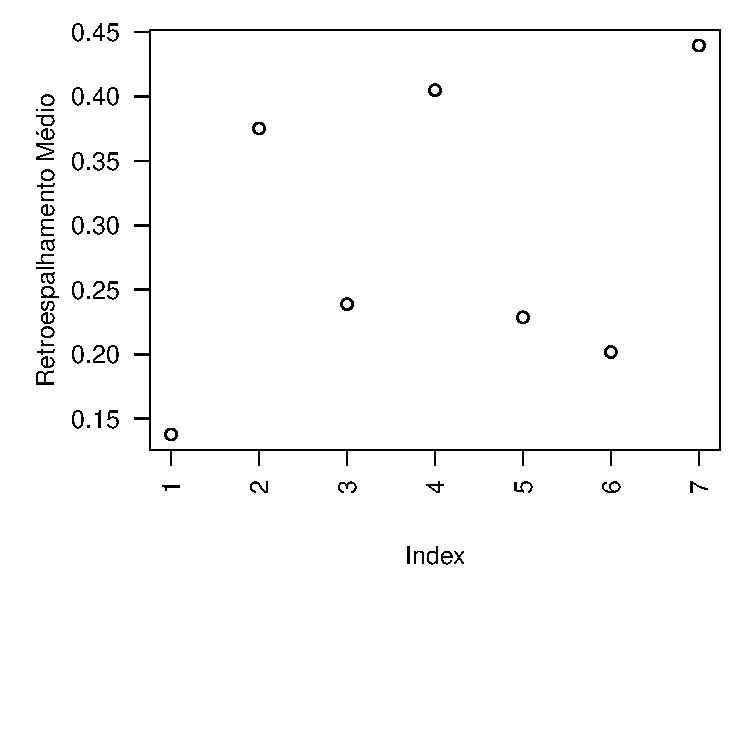
\includegraphics[width=1\linewidth]{figure/unnamed-chunk-57-1} 

\end{knitrout}

\end{columns}

\end{frame}
%===============================================================================%


%===============================================================================%
\begin{frame}[fragile]{Tipos de Gráficos - 2 variáveis: Dispersão (\emph{scatterplot})}

\begin{columns}[t]

\column{0.6\linewidth}

\begin{knitrout}\tiny
\definecolor{shadecolor}{rgb}{0.969, 0.969, 0.969}\color{fgcolor}\begin{kframe}
\begin{alltt}
\hlkwd{plot}\hlstd{(mean.bs,}\hlkwc{las}\hlstd{=}\hlnum{2}\hlstd{,}\hlkwc{ylab}\hlstd{=}\hlstr{"Retroespalhamento Médio"}\hlstd{,}\hlcom{#}
     \hlkwc{type}\hlstd{=}\hlstr{"p"}\hlstd{,}\hlkwc{xaxt}\hlstd{=}\hlstr{"n"}\hlstd{,}\hlkwc{xlab}\hlstd{=}\hlnum{NA}\hlstd{)}
\hlkwd{axis}\hlstd{(}\hlnum{1}\hlstd{,}\hlkwd{c}\hlstd{(}\hlnum{1}\hlopt{:}\hlnum{7}\hlstd{),}\hlkwc{labels}\hlstd{=}\hlkwd{names}\hlstd{(mean.bs),}\hlkwc{las}\hlstd{=}\hlnum{2}\hlstd{)}
\end{alltt}
\end{kframe}
\end{knitrout}

\column{0.4\linewidth}

\begin{knitrout}
\definecolor{shadecolor}{rgb}{0.969, 0.969, 0.969}\color{fgcolor}
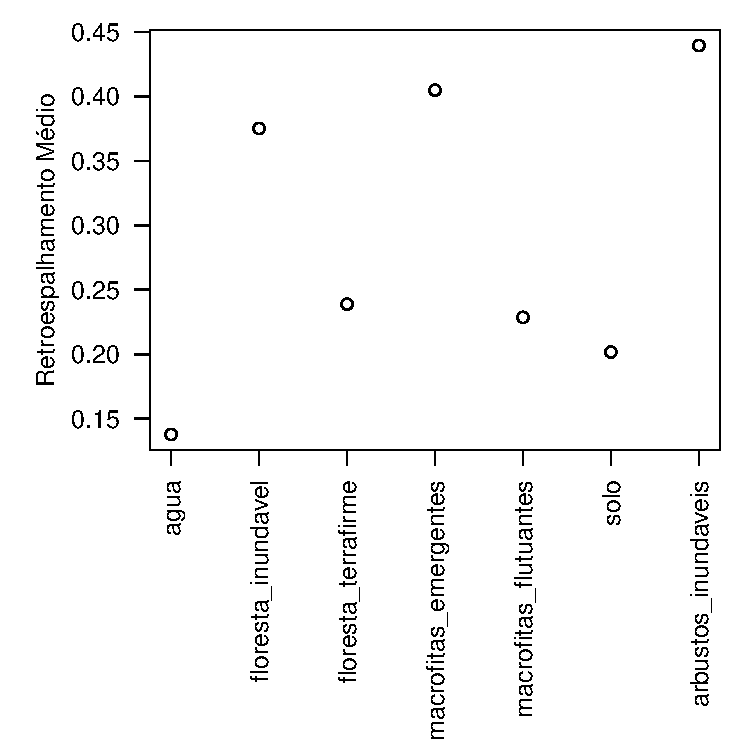
\includegraphics[width=1\linewidth]{figure/unnamed-chunk-59-1} 

\end{knitrout}

\end{columns}

\end{frame}
%===============================================================================%

%===============================================================================%
\begin{frame}[fragile]{Tipos de Gráficos - 2 variáveis: Dispersão (\emph{scatterplot})}

\begin{columns}[t]

\column{0.6\linewidth}

Incorreto, não existe continuidade entre as categorias.
\vfill

\begin{knitrout}\tiny
\definecolor{shadecolor}{rgb}{0.969, 0.969, 0.969}\color{fgcolor}\begin{kframe}
\begin{alltt}
\hlkwd{plot}\hlstd{(mean.bs,}\hlkwc{las}\hlstd{=}\hlnum{2}\hlstd{,}\hlkwc{ylab}\hlstd{=}\hlstr{"Retroespalhamento Médio"}\hlstd{,}\hlcom{#}
     \hlkwc{type}\hlstd{=}\hlstr{"l"}\hlstd{,}\hlkwc{xaxt}\hlstd{=}\hlstr{"n"}\hlstd{,}\hlkwc{xlab}\hlstd{=}\hlnum{NA}\hlstd{)}
\hlkwd{axis}\hlstd{(}\hlnum{1}\hlstd{,}\hlkwd{c}\hlstd{(}\hlnum{1}\hlopt{:}\hlnum{7}\hlstd{),}\hlkwc{labels}\hlstd{=}\hlkwd{names}\hlstd{(mean.bs),}\hlkwc{las}\hlstd{=}\hlnum{2}\hlstd{)}
\end{alltt}
\end{kframe}
\end{knitrout}

\column{0.4\linewidth}

\begin{knitrout}
\definecolor{shadecolor}{rgb}{0.969, 0.969, 0.969}\color{fgcolor}
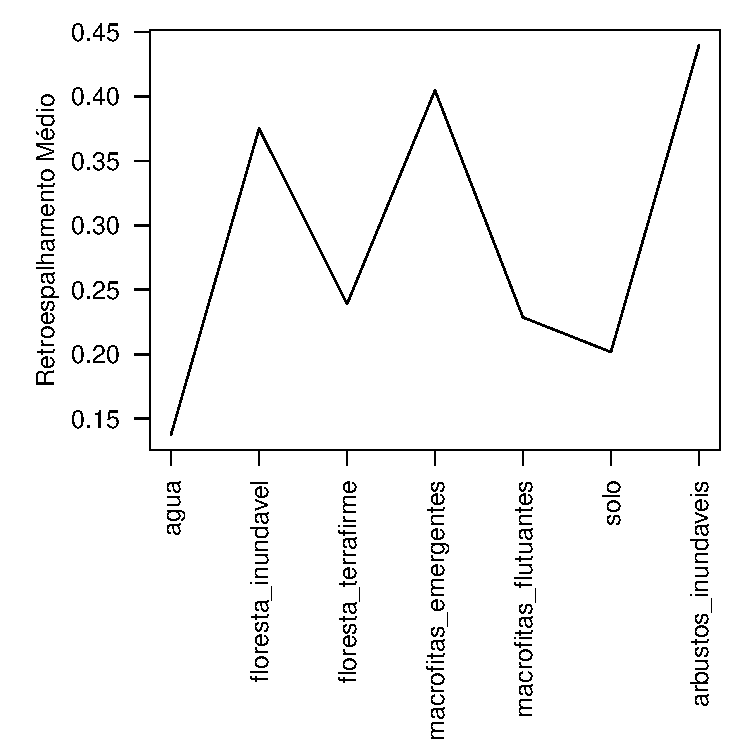
\includegraphics[width=1\linewidth]{figure/unnamed-chunk-61-1} 

\end{knitrout}

\end{columns}

\end{frame}
%===============================================================================

%===============================================================================%
\begin{frame}[fragile]{Tipos de Gráficos - 2 variáveis: Dispersão (\emph{scatterplot})}

\begin{columns}[t]

\column{0.6\linewidth}

\begin{knitrout}\tiny
\definecolor{shadecolor}{rgb}{0.969, 0.969, 0.969}\color{fgcolor}\begin{kframe}
\begin{alltt}
\hlkwd{plot}\hlstd{(mean.bs,}\hlkwc{las}\hlstd{=}\hlnum{2}\hlstd{,}\hlkwc{ylab}\hlstd{=}\hlstr{"Retroespalhamento Médio"}\hlstd{,}\hlkwc{type}\hlstd{=}\hlstr{"l"}\hlstd{,}\hlcom{#}
     \hlkwc{xaxt}\hlstd{=}\hlstr{"n"}\hlstd{,}\hlkwc{xlab}\hlstd{=}\hlnum{NA}\hlstd{)}
\hlkwd{axis}\hlstd{(}\hlnum{1}\hlstd{,}\hlkwd{c}\hlstd{(}\hlnum{1}\hlopt{:}\hlnum{7}\hlstd{),}\hlkwc{labels}\hlstd{=}\hlkwd{names}\hlstd{(mean.bs),}\hlkwc{las}\hlstd{=}\hlnum{2}\hlstd{)}
\hlkwd{library}\hlstd{(Hmisc)}
\hlkwd{errbar}\hlstd{(}\hlkwd{c}\hlstd{(}\hlnum{1}\hlopt{:}\hlnum{7}\hlstd{),mean.bs,}\hlkwc{yplus}\hlstd{=mean.bs}\hlopt{+}\hlstd{sd.bs,}\hlcom{#}
       \hlkwc{yminus}\hlstd{=mean.bs}\hlopt{-}\hlstd{sd.bs,}\hlkwc{lty}\hlstd{=}\hlnum{1}\hlstd{,}\hlkwc{xaxt}\hlstd{=}\hlstr{"n"}\hlstd{,}\hlkwc{xlab}\hlstd{=}\hlnum{NA}\hlstd{)}
\hlkwd{axis}\hlstd{(}\hlnum{1}\hlstd{,}\hlkwd{c}\hlstd{(}\hlnum{1}\hlopt{:}\hlnum{7}\hlstd{),}\hlkwc{labels}\hlstd{=}\hlkwd{names}\hlstd{(mean.bs),}\hlkwc{las}\hlstd{=}\hlnum{2}\hlstd{)}
\end{alltt}
\end{kframe}
\end{knitrout}

\column{0.4\linewidth}

\begin{knitrout}
\definecolor{shadecolor}{rgb}{0.969, 0.969, 0.969}\color{fgcolor}
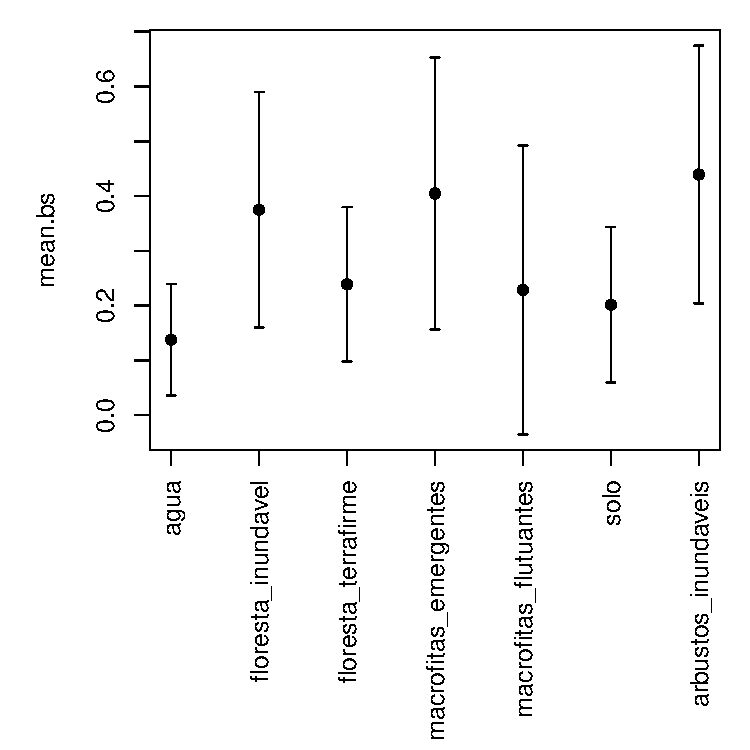
\includegraphics[width=1\linewidth]{figure/unnamed-chunk-63-1} 

\end{knitrout}

\end{columns}

\end{frame}
%===============================================================================%

%===============================================================================%
\begin{frame}[fragile]{Tipos de Gráficos - 2 variáveis: Dispersão (\emph{scatterplot})}

\begin{columns}[t]

\column{0.6\linewidth}

\begin{knitrout}\tiny
\definecolor{shadecolor}{rgb}{0.969, 0.969, 0.969}\color{fgcolor}\begin{kframe}
\begin{alltt}
\hlkwd{load}\hlstd{(}\hlstr{'rich+env_jun.Rdata'}\hlstd{)}
\hlkwd{plot}\hlstd{(rich.env.jun}\hlopt{$}\hlstd{p.tot,rich.env.jun}\hlopt{$}\hlstd{rich,}
     \hlkwc{xlab}\hlstd{=}\hlstr{"Fósforo Total"}\hlstd{,} \hlkwc{ylab} \hlstd{=} \hlstr{"Riqueza de Espécies"}\hlstd{)}
\hlcom{# A sintaxe de "em função de" (~) também pode ser usada}
\hlkwd{plot}\hlstd{(rich} \hlopt{~} \hlstd{p.tot,} \hlkwc{data}\hlstd{=rich.env.jun,}
     \hlkwc{xlab}\hlstd{=}\hlstr{"Fósforo Total"}\hlstd{,} \hlkwc{ylab} \hlstd{=} \hlstr{"Riqueza de Espécies"}\hlstd{)}
\end{alltt}
\end{kframe}
\end{knitrout}

\column{0.4\linewidth}

\begin{knitrout}
\definecolor{shadecolor}{rgb}{0.969, 0.969, 0.969}\color{fgcolor}
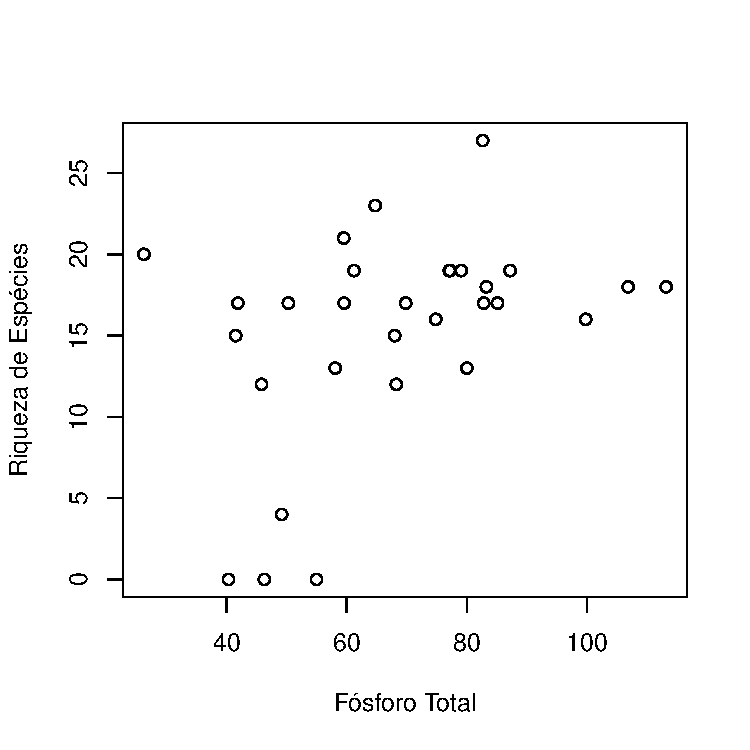
\includegraphics[width=1\linewidth]{figure/unnamed-chunk-65-1} 

\end{knitrout}

\end{columns}

\end{frame}
%===============================================================================%


%===============================================================================%
\begin{frame}{Tipos de Gráficos - 2 variáveis: Gráfico de Área}
  
\textbf{Área}
  
\begin{itemize}
  \item Pode ser visto como uma versão contínua do gráfico de barras \ldots \pause
  \vfill
  \item Mostra diferenças ponto a ponto, e cumulativas
  \vfill
  \item Não deve ser usado se a área sob a curva não fizer sentido para os dados plotados \pause
  \vfill
  \item A ordem do empilhamento pode afetar a percepção \pause
  \vfill
  \item se a variável x não for contínua, melhor usar barras empilhadas \pause
  
\end{itemize}

\end{frame} 
%===============================================================================%


%===============================================================================%
\begin{frame}[fragile]{Tipos de Gráficos - 2 variáveis: Gráfico de Área}

\begin{columns}[t]

\column{0.4\linewidth}

\begin{knitrout}\tiny
\definecolor{shadecolor}{rgb}{0.969, 0.969, 0.969}\color{fgcolor}\begin{kframe}
\begin{alltt}
\hlkwd{load}\hlstd{(}\hlstr{'npp_summary.Rdata'}\hlstd{)}
\hlkwd{library}\hlstd{(ggplot2)}
\hlkwd{ggplot}\hlstd{(npp.df,}\hlkwd{aes}\hlstd{(year,mean))} \hlopt{+}\hlcom{#}
  \hlkwd{geom_area}\hlstd{(}\hlkwc{fill}\hlstd{=}\hlstr{'gray50'}\hlstd{)} \hlopt{+}\hlcom{#}
  \hlkwd{xlab}\hlstd{(}\hlstr{"Ano"}\hlstd{)} \hlopt{+}\hlcom{#}
  \hlkwd{ylab}\hlstd{(}\hlstr{"Produtividade Primára (Tg/ano)"}\hlstd{)}
\end{alltt}
\end{kframe}
\end{knitrout}

\column{0.6\linewidth}

\begin{knitrout}
\definecolor{shadecolor}{rgb}{0.969, 0.969, 0.969}\color{fgcolor}
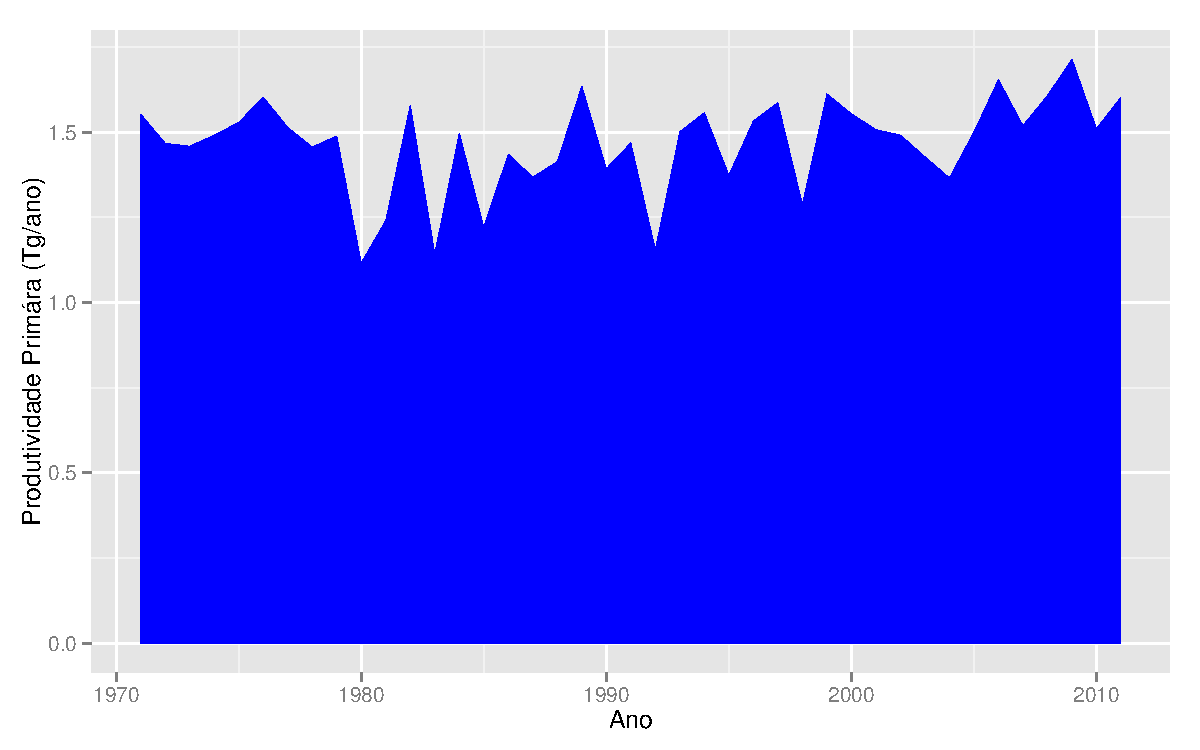
\includegraphics[width=1\linewidth]{figure/unnamed-chunk-67-1} 

\end{knitrout}

\end{columns}

\end{frame}
%===============================================================================%

%===============================================================================%
\begin{frame}[fragile]{Tipos de Gráficos - 2 variáveis: Gráfico de Área}

\begin{columns}[t]

\column{0.4\linewidth}

\begin{knitrout}\tiny
\definecolor{shadecolor}{rgb}{0.969, 0.969, 0.969}\color{fgcolor}\begin{kframe}
\begin{alltt}
\hlkwd{library}\hlstd{(ggplot2)}
\hlkwd{ggplot}\hlstd{(npp.df,}\hlkwd{aes}\hlstd{(year,mean))} \hlopt{+} \hlcom{#}
  \hlkwd{geom_area}\hlstd{(}\hlkwc{fill}\hlstd{=}\hlstr{'blue'}\hlstd{)} \hlopt{+}\hlcom{#}
  \hlkwd{xlab}\hlstd{(}\hlstr{"Ano"}\hlstd{)} \hlopt{+} \hlcom{#}
  \hlkwd{ylab}\hlstd{(}\hlstr{"Produtividade Primária (Tg/ano)"}\hlstd{)}

\hlkwd{ggplot}\hlstd{(npp.df,}\hlkwd{aes}\hlstd{(}\hlkwd{as.factor}\hlstd{(year),mean))} \hlopt{+}
  \hlkwd{geom_bar}\hlstd{(}\hlkwc{fill}\hlstd{=}\hlstr{'blue'}\hlstd{)} \hlopt{+}\hlkwd{xlab}\hlstd{(}\hlstr{"Ano"}\hlstd{)} \hlopt{+}
  \hlkwd{ylab}\hlstd{(}\hlstr{"Produtividade Primária (Tg/ano)"}\hlstd{)} \hlopt{+}
  \hlkwd{theme}\hlstd{(}\hlkwc{axis.text.x} \hlstd{=} \hlkwd{element_text}\hlstd{(}\hlkwc{angle} \hlstd{=} \hlnum{90}\hlstd{,} \hlkwc{hjust} \hlstd{=} \hlnum{1}\hlstd{))}
\end{alltt}
\end{kframe}
\end{knitrout}

\column{0.6\linewidth}

\begin{knitrout}
\definecolor{shadecolor}{rgb}{0.969, 0.969, 0.969}\color{fgcolor}
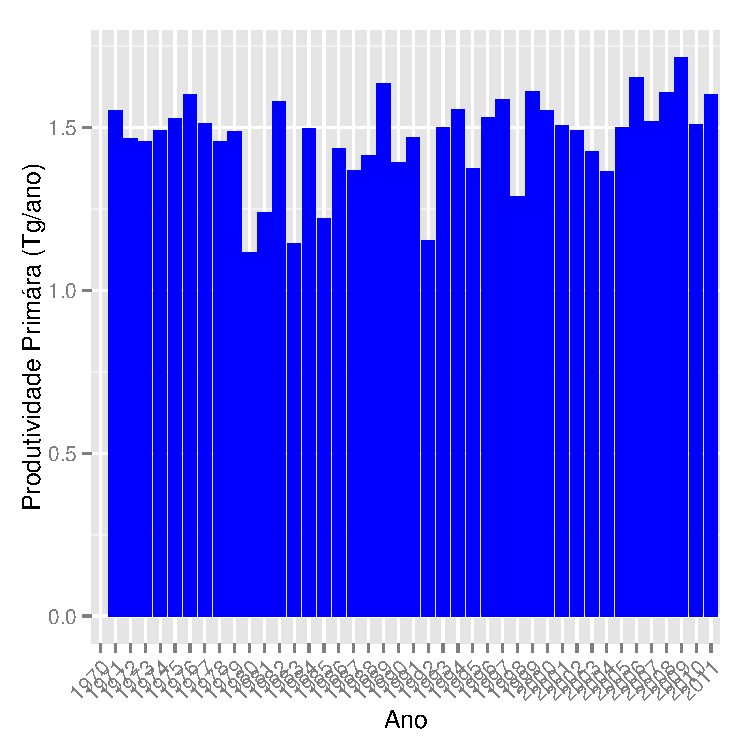
\includegraphics[width=1\linewidth]{figure/unnamed-chunk-69-1} 

\end{knitrout}

\end{columns}

\end{frame}
%===============================================================================%



%===============================================================================%
\begin{frame}[fragile]{Tipos de Gráficos - 2 variáveis: Gráfico de Área}

\url{http://www.leancrew.com/all-this/2011/11/i-hate-stacked-area-charts/}

\end{frame}
%===============================================================================%


%===============================================================================%
\begin{frame}{Tipos de Gráficos - 2 variáveis: \emph{Boxplot}}

\textbf{Boxplot}

\begin{itemize}
  \item Usado para combinações entre variáveis contínuas e categóricas \ldots \pause
  \vfill
  \item Na opinião de muitos, um dos gráficos mais informativos que existem \ldots \pause
  \vfill
  \item Combina as propriedades de um histograma e de um scatterplot \pause
  \vfill
  \item Faz uso dos quantis para uma descrição robusta dos dados 
\end{itemize}

\end{frame} 
%===============================================================================%



%===============================================================================%
\begin{frame}[fragile]{Tipos de Gráficos - 2 variáveis: \emph{Boxplot}}

\centering
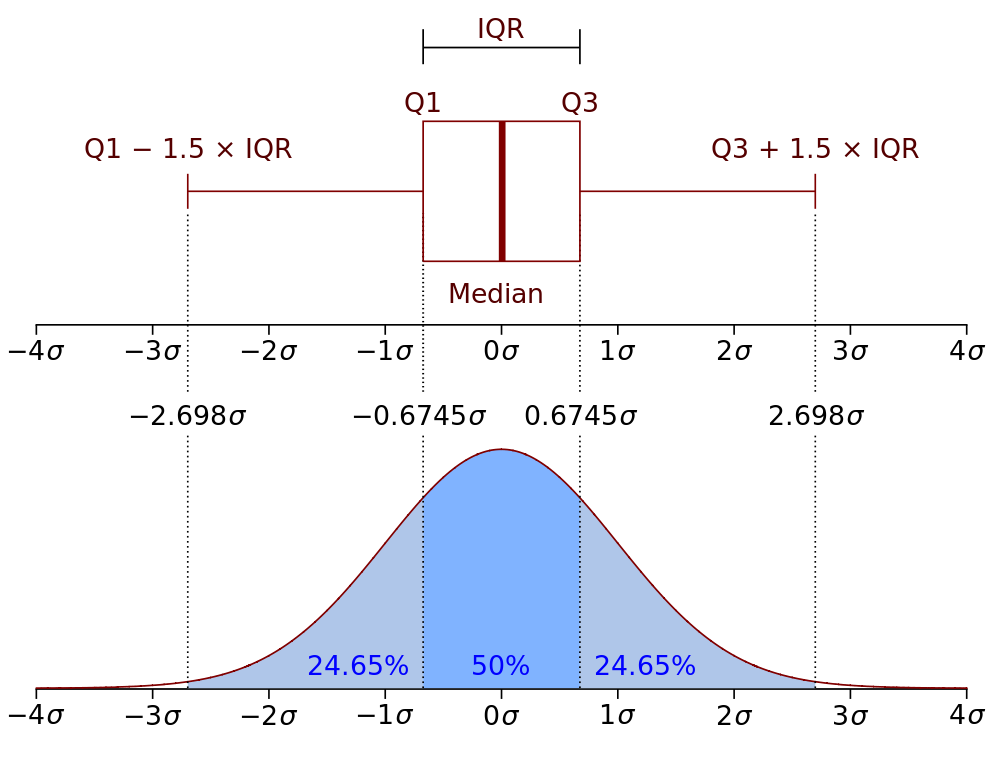
\includegraphics[width=0.65\linewidth]{C:/Users/thiago/OneDrive/UNESP/Pos_graduacao/Eco/2015/Estatistica_2015/Aulas/Aula_3_EDA_Graph/figs/boxp.png}

\end{frame}
%===============================================================================%

%===============================================================================%
\begin{frame}[fragile]{Tipos de Gráficos - 2 variáveis: \emph{Boxplot}}


\begin{columns}[t]

\column{0.5\linewidth}

\begin{knitrout}
\definecolor{shadecolor}{rgb}{0.969, 0.969, 0.969}\color{fgcolor}
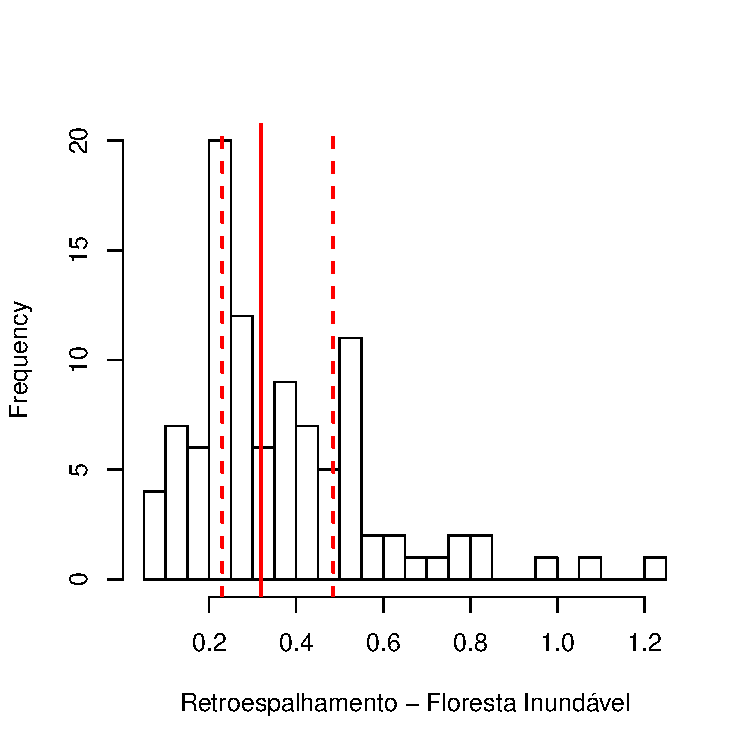
\includegraphics[width=1\linewidth]{figure/unnamed-chunk-70-1} 

\end{knitrout}


\column{0.5\linewidth}

\begin{knitrout}
\definecolor{shadecolor}{rgb}{0.969, 0.969, 0.969}\color{fgcolor}
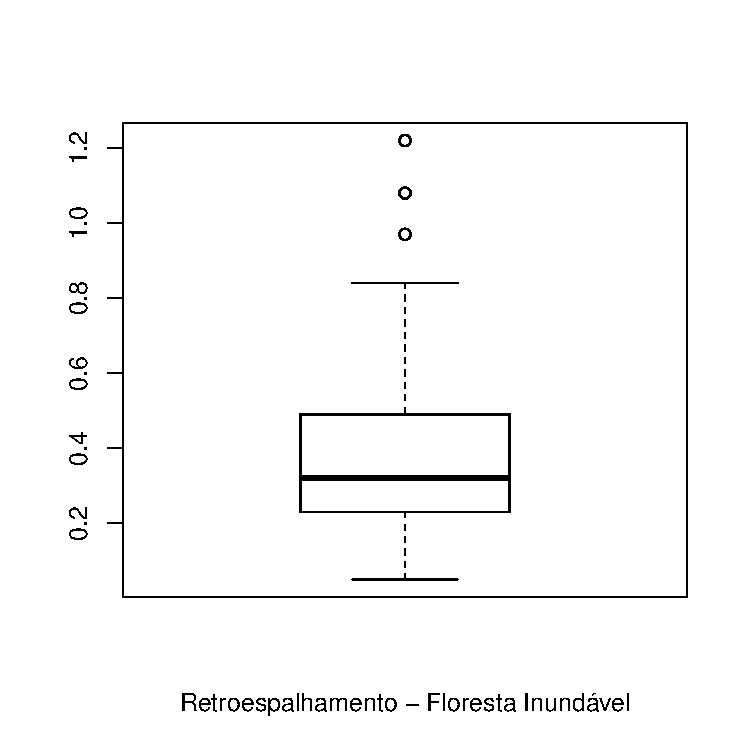
\includegraphics[width=1\linewidth]{figure/unnamed-chunk-71-1} 

\end{knitrout}

\end{columns}

\end{frame}
%===============================================================================%


%===============================================================================%
\begin{frame}[fragile]{Tipos de Gráficos - 2 variáveis: \emph{Boxplot}}


\begin{columns}[t]

\column{0.49\linewidth}

\begin{knitrout}\tiny
\definecolor{shadecolor}{rgb}{0.969, 0.969, 0.969}\color{fgcolor}\begin{kframe}
\begin{alltt}
\hlkwd{boxplot}\hlstd{(sigma0} \hlopt{~} \hlstd{classe,} \hlkwc{data}\hlstd{=plot.data,} \hlkwc{las}\hlstd{=}\hlnum{2}\hlstd{)}

\hlcom{#linha central: mediana}
\hlcom{#}
\hlcom{#caixa : quartis}
\hlcom{#}
\hlcom{#linhas verticais: valor mais alto/baixo dentro da }
\hlcom{# distância quartil+/-1.5*distancia interquartil}
\hlcom{#}
\hlcom{# pontos: outliers, tudo que for maior }
\hlcom{# do que quartil +/- 1.5 quartil}
\end{alltt}
\end{kframe}
\end{knitrout}

\scriptsize{Superposição da distância interquartil é um indício de diferença/separabilidade}

\column{0.6\linewidth}

\begin{knitrout}
\definecolor{shadecolor}{rgb}{0.969, 0.969, 0.969}\color{fgcolor}
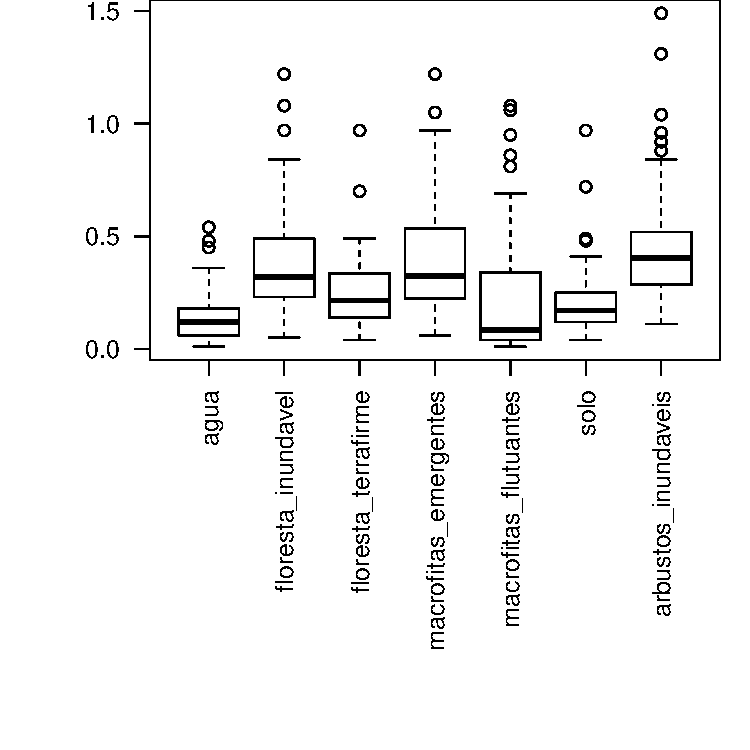
\includegraphics[width=1\linewidth]{figure/unnamed-chunk-73-1} 

\end{knitrout}

\end{columns}

\end{frame}
%===============================================================================%


%===============================================================================%
\begin{frame}{Tipos de Gráficos - 2 variáveis: \emph{Violin Plot}}
\setbeamercovered{transparent}
  
\begin{itemize}
  \item Tentativa de ir além do boxplot \ldots \pause
  \vfill
  \item Combina as propriedades de um gráfico de densidades e de um scatterplot\pause
  \vfill
  \item Pode ficar estranho se as distribuições não forem bem-comportadas 
\end{itemize}

\end{frame} 
%===============================================================================%


%===============================================================================%
\begin{frame}[fragile]{Tipos de Gráficos - 2 variáveis: \emph{Violin Plot}}

\begin{columns}[t]

\column{0.49\linewidth}

\begin{knitrout}\tiny
\definecolor{shadecolor}{rgb}{0.969, 0.969, 0.969}\color{fgcolor}\begin{kframe}
\begin{alltt}
\hlkwd{ggplot}\hlstd{(plot.data,}\hlkwd{aes}\hlstd{(classe,sigma0))} \hlopt{+}\hlcom{#}
  \hlkwd{geom_boxplot}\hlstd{()} \hlopt{+} \hlkwd{theme}\hlstd{(}\hlkwc{axis.text.x} \hlstd{=} \hlkwd{element_text}\hlstd{(}\hlkwc{angle} \hlstd{=} \hlnum{90}\hlstd{,} \hlkwc{hjust} \hlstd{=} \hlnum{1}\hlstd{))}
\end{alltt}
\end{kframe}
\end{knitrout}

\column{0.6\linewidth}

\begin{knitrout}
\definecolor{shadecolor}{rgb}{0.969, 0.969, 0.969}\color{fgcolor}
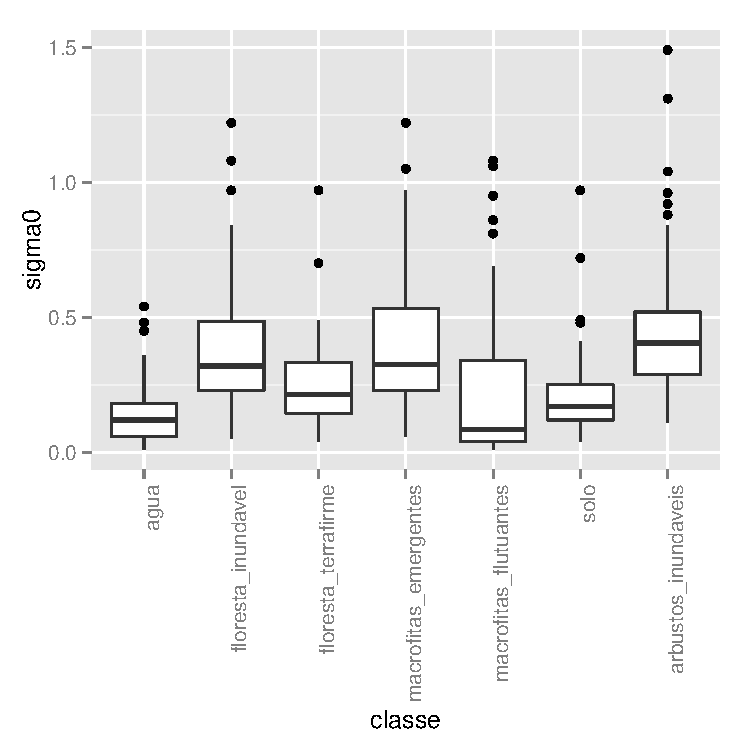
\includegraphics[width=1\linewidth]{figure/unnamed-chunk-75-1} 

\end{knitrout}

\end{columns}

\end{frame}
%===============================================================================%


%===============================================================================%
\begin{frame}[fragile]{Tipos de Gráficos - 2 variáveis: \emph{Violin Plot}}

\begin{columns}[t]

\column{0.49\linewidth}

\begin{knitrout}\tiny
\definecolor{shadecolor}{rgb}{0.969, 0.969, 0.969}\color{fgcolor}\begin{kframe}
\begin{alltt}
\hlkwd{ggplot}\hlstd{(plot.data,}\hlkwd{aes}\hlstd{(classe,sigma0))} \hlopt{+}\hlcom{#}
  \hlkwd{geom_boxplot}\hlstd{()} \hlopt{+}\hlcom{#}
  \hlkwd{theme}\hlstd{(}\hlkwc{axis.text.x} \hlstd{=} \hlkwd{element_text}\hlstd{(}\hlkwc{angle} \hlstd{=} \hlnum{90}\hlstd{,} \hlkwc{hjust} \hlstd{=} \hlnum{1}\hlstd{))}
\hlkwd{ggplot}\hlstd{(plot.data,}\hlkwd{aes}\hlstd{(classe,sigma0))} \hlopt{+}\hlcom{#}
  \hlkwd{geom_violin}\hlstd{()} \hlopt{+}\hlcom{#}
  \hlkwd{theme}\hlstd{(}\hlkwc{axis.text.x} \hlstd{=} \hlkwd{element_text}\hlstd{(}\hlkwc{angle} \hlstd{=} \hlnum{90}\hlstd{,} \hlkwc{hjust} \hlstd{=} \hlnum{1}\hlstd{))}
\end{alltt}
\end{kframe}
\end{knitrout}

\column{0.6\linewidth}

\begin{knitrout}
\definecolor{shadecolor}{rgb}{0.969, 0.969, 0.969}\color{fgcolor}
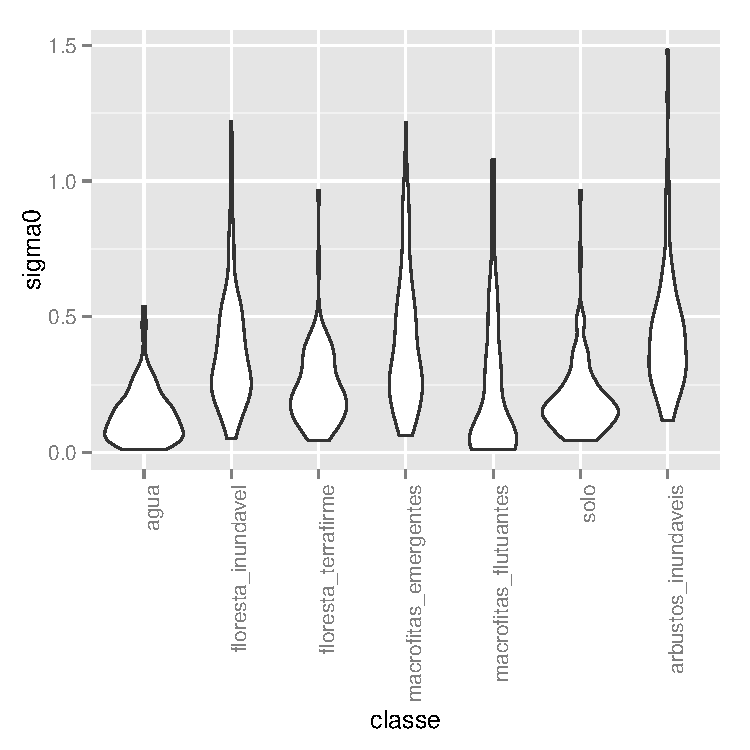
\includegraphics[width=1\linewidth]{figure/unnamed-chunk-77-1} 

\end{knitrout}

\end{columns}

\end{frame}
%===============================================================================%

%===============================================================================%
\begin{frame}{Combinando mais de duas variáveis \dots sem usar ``3D''}
\setbeamercovered{transparent}
  
\begin{itemize}
  \item Gráficos ``3D'' são dependentes de perspectiva, e não enfatizam bem as diferenças \pause
  \vfill
  \item São uma boa ferramenta de visualização se puderem ser manipulados \pause
  \vfill
  \item Mas para exibição em papel, dificultam a interpretação \pause
  \vfill
  \item Ao invés de usar múltiplos eixos, podemos explorar as relações entre cor, forma e tamanho dos objetos plotados 
\end{itemize}

\end{frame} 
%===============================================================================%


%===============================================================================%
\begin{frame}[fragile]{Tipos de Gráficos - 2 variáveis}

\begin{columns}[t]

\column{0.49\linewidth}

\begin{knitrout}\tiny
\definecolor{shadecolor}{rgb}{0.969, 0.969, 0.969}\color{fgcolor}\begin{kframe}
\begin{alltt}
\hlkwd{ggplot}\hlstd{(rich.env.jun,}\hlkwd{aes}\hlstd{(p.tot,n.tot))} \hlopt{+}\hlcom{#}
  \hlkwd{geom_point}\hlstd{(}\hlkwc{size}\hlstd{=}\hlnum{3}\hlstd{)} \hlopt{+}\hlcom{#}
  \hlkwd{ylab}\hlstd{(}\hlstr{"Nitrogênio Total"}\hlstd{)} \hlopt{+}\hlcom{#}
  \hlkwd{xlab}\hlstd{(}\hlstr{"Fósforo Total"}\hlstd{)} \hlopt{+}\hlcom{#}
  \hlkwd{theme_bw}\hlstd{()}
\end{alltt}
\end{kframe}
\end{knitrout}

\column{0.6\linewidth}

\begin{knitrout}
\definecolor{shadecolor}{rgb}{0.969, 0.969, 0.969}\color{fgcolor}
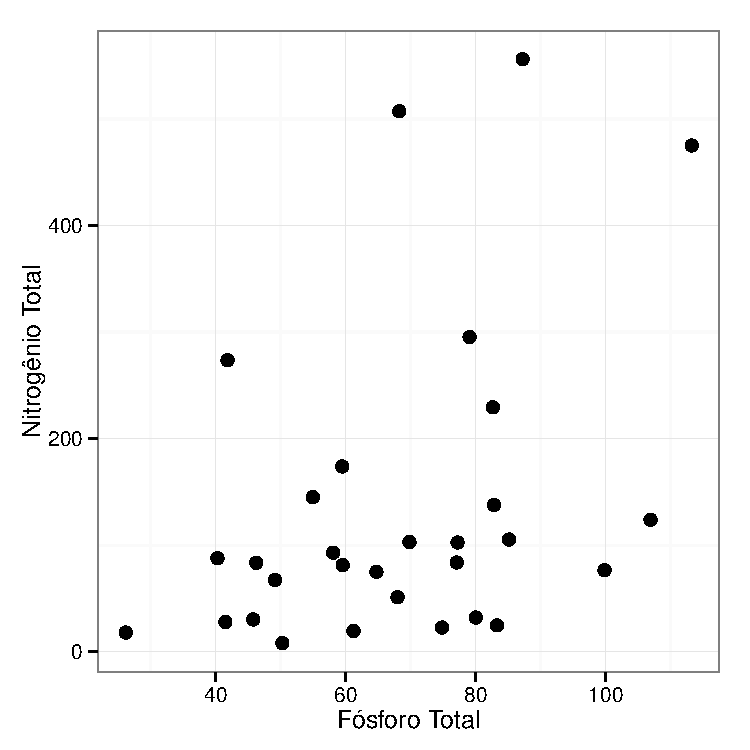
\includegraphics[width=1\linewidth]{figure/unnamed-chunk-79-1} 

\end{knitrout}

\end{columns}

\end{frame}
%===============================================================================%

%===============================================================================%
\begin{frame}[fragile]{Tipos de Gráficos - 3 variáveis}

\begin{columns}[t]

\column{0.49\linewidth}

\begin{knitrout}\tiny
\definecolor{shadecolor}{rgb}{0.969, 0.969, 0.969}\color{fgcolor}\begin{kframe}
\begin{alltt}
\hlkwd{ggplot}\hlstd{(rich.env.jun,}\hlkwd{aes}\hlstd{(p.tot,n.tot))} \hlopt{+}\hlcom{#}
  \hlkwd{geom_point}\hlstd{(}\hlkwc{size}\hlstd{=}\hlnum{3}\hlstd{)} \hlopt{+}\hlcom{#}
  \hlkwd{ylab}\hlstd{(}\hlstr{"Nitrogênio Total"}\hlstd{)} \hlopt{+}\hlcom{#}
  \hlkwd{xlab}\hlstd{(}\hlstr{"Fósforo Total"}\hlstd{)} \hlopt{+}\hlcom{#}
  \hlkwd{theme_bw}\hlstd{()}
\hlkwd{ggplot}\hlstd{(rich.env.jun,}\hlkwd{aes}\hlstd{(p.tot,n.tot))} \hlopt{+}\hlcom{#}
  \hlkwd{geom_point}\hlstd{(}\hlkwd{aes}\hlstd{(}\hlkwc{size}\hlstd{=rich))} \hlopt{+}\hlcom{#}
  \hlkwd{ylab}\hlstd{(}\hlstr{"Nitrogênio Total"}\hlstd{)} \hlopt{+}\hlcom{#}
  \hlkwd{xlab}\hlstd{(}\hlstr{"Fósforo Total"}\hlstd{)} \hlopt{+}\hlcom{#}
  \hlkwd{theme_bw}\hlstd{()}
\end{alltt}
\end{kframe}
\end{knitrout}

\column{0.6\linewidth}

\begin{knitrout}
\definecolor{shadecolor}{rgb}{0.969, 0.969, 0.969}\color{fgcolor}
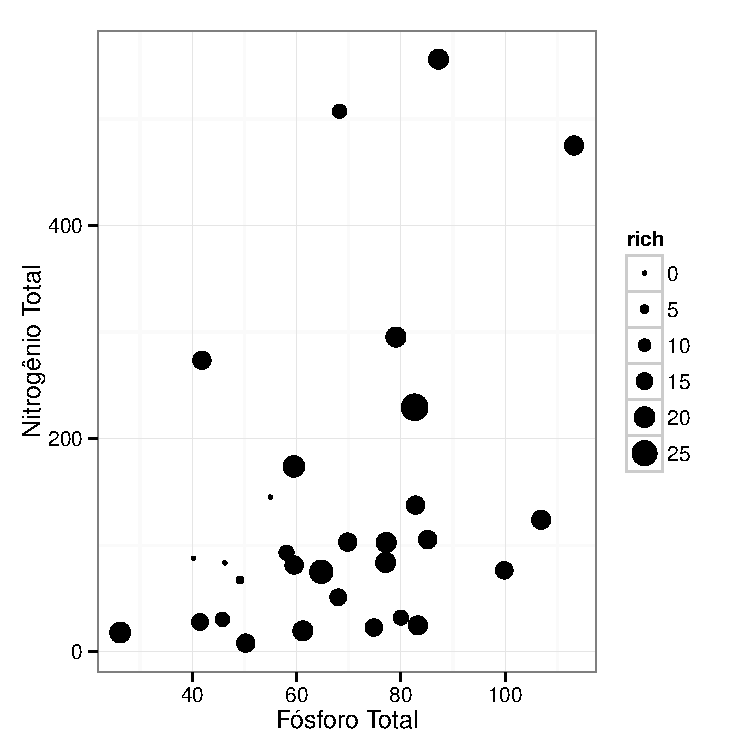
\includegraphics[width=1\linewidth]{figure/unnamed-chunk-81-1} 

\end{knitrout}

\end{columns}

\end{frame}
%===============================================================================%

%===============================================================================%
\begin{frame}[fragile]{Tipos de Gráficos - 4 variáveis}

\begin{columns}[t]


\column{0.49\linewidth}

\begin{knitrout}\tiny
\definecolor{shadecolor}{rgb}{0.969, 0.969, 0.969}\color{fgcolor}\begin{kframe}
\begin{alltt}
\hlkwd{ggplot}\hlstd{(rich.env.jun,}\hlkwd{aes}\hlstd{(p.tot,n.tot))} \hlopt{+}\hlcom{#}
  \hlkwd{geom_point}\hlstd{(}\hlkwc{size}\hlstd{=}\hlnum{3}\hlstd{)} \hlopt{+}\hlcom{#}
  \hlkwd{ylab}\hlstd{(}\hlstr{"Nitrogênio Total"}\hlstd{)} \hlopt{+}\hlcom{#}
  \hlkwd{xlab}\hlstd{(}\hlstr{"Fósforo Total"}\hlstd{)} \hlopt{+}\hlcom{#}
  \hlkwd{theme_bw}\hlstd{()}
\hlkwd{ggplot}\hlstd{(rich.env.jun,}\hlkwd{aes}\hlstd{(p.tot,n.tot))} \hlopt{+}\hlcom{#}
  \hlkwd{geom_point}\hlstd{(}\hlkwd{aes}\hlstd{(}\hlkwc{size}\hlstd{=rich))} \hlopt{+}\hlcom{#}
  \hlkwd{ylab}\hlstd{(}\hlstr{"Nitrogênio Total"}\hlstd{)} \hlopt{+}\hlcom{#}
  \hlkwd{xlab}\hlstd{(}\hlstr{"Fósforo Total"}\hlstd{)} \hlopt{+}\hlcom{#}
  \hlkwd{theme_bw}\hlstd{()}
\hlkwd{ggplot}\hlstd{(rich.env.jun,}\hlkwd{aes}\hlstd{(p.tot,n.tot))} \hlopt{+}\hlcom{#}
  \hlkwd{geom_point}\hlstd{(}\hlkwd{aes}\hlstd{(}\hlkwc{color}\hlstd{=rich,} \hlkwc{size}\hlstd{=prof}\hlopt{*-}\hlnum{1}\hlstd{))} \hlopt{+}\hlcom{#}
  \hlkwd{ylab}\hlstd{(}\hlstr{"Nitrogênio Total"}\hlstd{)} \hlopt{+}\hlcom{#}
  \hlkwd{xlab}\hlstd{(}\hlstr{"Fósforo Total"}\hlstd{)} \hlopt{+}\hlcom{#}
  \hlkwd{theme_bw}\hlstd{()}
\end{alltt}
\end{kframe}
\end{knitrout}

\column{0.6\linewidth}

\begin{knitrout}
\definecolor{shadecolor}{rgb}{0.969, 0.969, 0.969}\color{fgcolor}
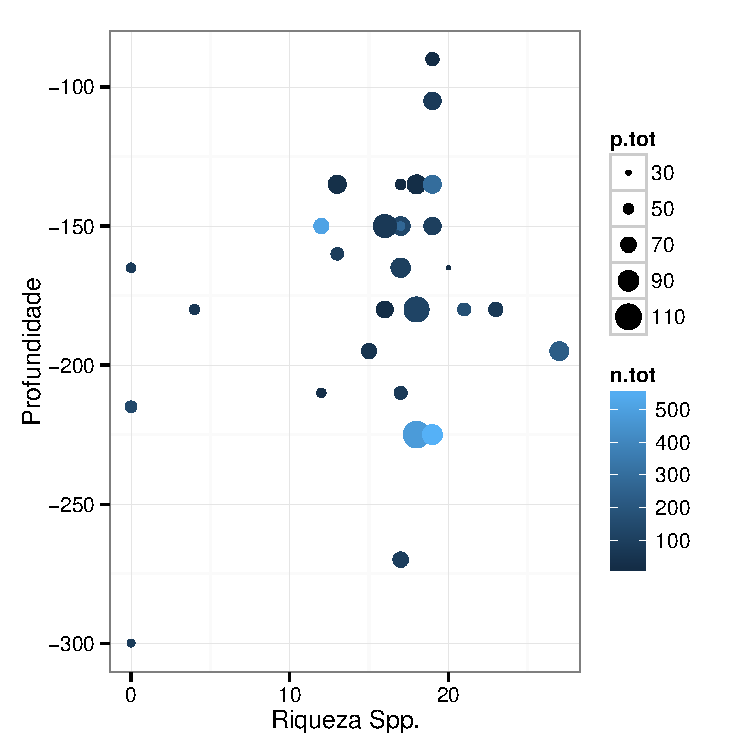
\includegraphics[width=1\linewidth]{figure/unnamed-chunk-83-1} 

\end{knitrout}

\end{columns}

\end{frame}
%===============================================================================%

%===============================================================================%
\begin{frame}[fragile]{Tipos de Gráficos - 5 variáveis}

\begin{columns}[t]


\column{0.49\linewidth}


\begin{knitrout}\tiny
\definecolor{shadecolor}{rgb}{0.969, 0.969, 0.969}\color{fgcolor}\begin{kframe}
\begin{alltt}
\hlkwd{ggplot}\hlstd{(rich.env.jun,}\hlkwd{aes}\hlstd{(p.tot,n.tot))} \hlopt{+}\hlcom{#}
  \hlkwd{geom_point}\hlstd{(}\hlkwc{size}\hlstd{=}\hlnum{3}\hlstd{)} \hlopt{+}\hlcom{#}
  \hlkwd{ylab}\hlstd{(}\hlstr{"Nitrogênio Total"}\hlstd{)} \hlopt{+}\hlcom{#}
  \hlkwd{xlab}\hlstd{(}\hlstr{"Fósforo Total"}\hlstd{)} \hlopt{+}\hlcom{#}
  \hlkwd{theme_bw}\hlstd{()}
\hlkwd{ggplot}\hlstd{(rich.env.jun,}\hlkwd{aes}\hlstd{(p.tot,n.tot))} \hlopt{+}\hlcom{#}
  \hlkwd{geom_point}\hlstd{(}\hlkwd{aes}\hlstd{(}\hlkwc{size}\hlstd{=rich))} \hlopt{+}\hlcom{#}
  \hlkwd{ylab}\hlstd{(}\hlstr{"Nitrogênio Total"}\hlstd{)} \hlopt{+}\hlcom{#}
  \hlkwd{xlab}\hlstd{(}\hlstr{"Fósforo Total"}\hlstd{)} \hlopt{+}\hlcom{#}
  \hlkwd{theme_bw}\hlstd{()}
\hlkwd{ggplot}\hlstd{(rich.env.jun,}\hlkwd{aes}\hlstd{(rich,prof))} \hlopt{+}\hlcom{#}
  \hlkwd{geom_point}\hlstd{(}\hlkwd{aes}\hlstd{(}\hlkwc{color}\hlstd{=n.tot,} \hlkwc{size}\hlstd{=p.tot))} \hlopt{+}\hlcom{#}
  \hlkwd{ylab}\hlstd{(}\hlstr{"Profundidade"}\hlstd{)} \hlopt{+}\hlcom{#}
  \hlkwd{xlab}\hlstd{(}\hlstr{"Riqueza Spp."}\hlstd{)} \hlopt{+}\hlcom{#}
  \hlkwd{theme_bw}\hlstd{()}
\hlkwd{ggplot}\hlstd{(rich.env.jun,}\hlkwd{aes}\hlstd{(rich,prof))} \hlopt{+}\hlcom{#}
  \hlkwd{geom_point}\hlstd{(}\hlkwd{aes}\hlstd{(}\hlkwc{color}\hlstd{=n.tot,} \hlkwc{size}\hlstd{=p.tot,} \hlkwc{shape}\hlstd{=clayfac))} \hlopt{+}\hlcom{#}
  \hlkwd{ylab}\hlstd{(}\hlstr{"Profundidade"}\hlstd{)} \hlopt{+}\hlcom{#}
  \hlkwd{xlab}\hlstd{(}\hlstr{"Riqueza Spp."}\hlstd{)} \hlopt{+}\hlcom{#}
  \hlkwd{theme_bw}\hlstd{()}
\end{alltt}
\end{kframe}
\end{knitrout}

\column{0.6\linewidth}

\begin{knitrout}
\definecolor{shadecolor}{rgb}{0.969, 0.969, 0.969}\color{fgcolor}
\includegraphics[width=1\linewidth]{figure/unnamed-chunk-86-1} 

\end{knitrout}

\end{columns}

\end{frame}
%===============================================================================%

%===============================================================================%
\begin{frame}{Elementos de um bom gráfico}
  
\begin{itemize}
  \item Foco na informação que se quer enfatizar \pause
  \vfill
  \item Quanto menor a razão tinta/papel, melhor \pause
  \vfill
  \item Selecione e ordene suas variáveis de acordo com a pergunta a ser respondida \pause
  \vfill
  \item Cores e formas só devem ser usadas se também trouxerem informação! \pause
\end{itemize}

\end{frame} 
%===============================================================================%

%===============================================================================%
\begin{frame}{Qual a pergunta a ser respondida?}

Diferença entre classes, para cada polarização?


\begin{knitrout}
\definecolor{shadecolor}{rgb}{0.969, 0.969, 0.969}\color{fgcolor}
\includegraphics[width=1.1\linewidth]{figure/unnamed-chunk-87-1} 

\end{knitrout}
\end{frame}
%===============================================================================%


%===============================================================================%
\begin{frame}{Qual a pergunta a ser respondida?}

Ou a diferença entre polarizações, para cada classe?


\begin{knitrout}
\definecolor{shadecolor}{rgb}{0.969, 0.969, 0.969}\color{fgcolor}
\includegraphics[width=1\linewidth]{figure/unnamed-chunk-88-1} 

\end{knitrout}
\end{frame}
%===============================================================================%

%===============================================================================%
\begin{frame}{Tipos de Gráficos}

\begin{columns}[T]


\column{0.5\linewidth}

\scriptsize{Isso é melhor \ldots}

\bigskip

\includegraphics[width=1\linewidth]{C:/Users/thiago/OneDrive/UNESP/Pos_graduacao/Eco/2015/Estatistica_2015/Aulas/Aula_3_EDA_Graph/figs/unnamed-chunk-72.pdf}

\pause

\column{0.5\linewidth}

\scriptsize{\ldots do que isso!}

\vfill

\includegraphics[width=1\linewidth]{C:/Users/thiago/OneDrive/UNESP/Pos_graduacao/Eco/2015/Estatistica_2015/Aulas/Aula_3_EDA_Graph/figs/badplot.pdf}

\end{columns}

\end{frame}
%===============================================================================%



\end{document}
